\documentclass[11pt]{amsart}
\ifdefined\pdfinfoomitdate\pdfinfoomitdate=1\relax\pdftrailerid{}\fi
\usepackage[T1]{fontenc}
\usepackage{lmodern,amsmath,amssymb,amsthm,mathtools,booktabs}
\usepackage[expansion=false]{microtype}
\usepackage{tikz}
\raggedbottom
\setlength{\emergencystretch}{2em}
\usepackage[margin=1in]{geometry}
\usepackage[numbers,sort&compress]{natbib}
\usepackage[hidelinks,hypertexnames=true]{hyperref}
\urlstyle{same}
\numberwithin{equation}{section}
\newtheorem{theorem}{Theorem}[section]
\newtheorem{proposition}[theorem]{Proposition}
\newtheorem{lemma}[theorem]{Lemma}
\newtheorem{corollary}[theorem]{Corollary}
\theoremstyle{definition}
\newtheorem{definition}[theorem]{Definition}
\theoremstyle{remark}
\newtheorem{remark}[theorem]{Remark}
\newcommand{\dd}{\,\mathrm{d}}
\newcommand{\eps}{\varepsilon}
\newcommand{\sgn}{\operatorname{sgn}}
\newcommand{\supp}{\operatorname{supp}}
\newcommand{\LieM}{\operatorname{Lie}_{M}}
\newcommand{\Tr}{\mathcal{T}}
\newcommand{\oscD}{\mathcal{D}}
\setcounter{tocdepth}{1}

\hypersetup{pdfauthor={Haibo Lu},pdftitle={Positive valleys and hyperbolic limit cycles in classical Lienard systems with a k-term primitive},
  pdfsubject={Positive minima, sparse polynomial primitives and finite return matching}}
\title[Positive valleys in sparse classical Li\'enard systems]{Positive valleys and hyperbolic limit cycles\\
in classical Li\'enard systems with a $k$-term primitive}
\author{Haibo Lu}
\address{Shanghai Institute of Technology}
\date{November 27, 2026}
\thanks{ORCID: \href{https://orcid.org/0009-0000-2717-5968}{0009-0000-2717-5968}.}
\subjclass[2020]{34C07, 34C23, 34E15}
\keywords{Classical Li\'enard system, sparse polynomial primitive, hyperbolic limit cycle, half-return map, slow divergence integral}

\begin{document}
\begin{abstract}
For every $k\ge10$ there is a support of $k$ positive integer powers
on which a nonempty open set of primitives $F$ gives at least $4k-17$
simultaneous hyperbolic limit cycles of the classical system
$\dot x=y-F(x)$, $\dot y=-x$. Published averaging constructions give
$k-1$ hyperbolic cycles. Counting powers in a construction from Lu's
fixed-degree preprint gives an asymptotic lower bound of $11/3$ cycles
per primitive term. Here each block of four new powers adds sixteen
cycles to the guaranteed count, raising that asymptotic bound to four.

A positive valley is a local minimum above zero in the even profile
obtained by reflecting and rescaling the two halves of the system.
Between the minimum and the preceding maximum, a return from the
positive axis and a trajectory entering from infinity sample different
rising arcs. With four suitably chosen new powers we obtain six changes
of the ordinary return comparison. The incoming comparison gives six
changes at positive heights and four at negative heights. Matching the
two halves at common finite launches yields the cycles. For profiles
with factors quadratic in $r^p$, the minimum has height $\sim\eta$ as
$\eta\downarrow0$. A negative first variation at some incoming height
$-H<0$ occurs precisely above an odd amplitude
$q_c(\eta)\sim K_{d,p}\eta^{1/2+1/d}$, where $d$ is the lowest even
power. This family gives ten-term examples with at least sixteen hyperbolic
cycles in each of degrees $22$ and $26$.
\end{abstract}
\maketitle

\section{How many cycles can a sparse primitive produce?}\label{sec:intro}
Fix the restoring force $x$ and consider the classical Li\'enard system
\begin{equation}\label{eq:lienard}
 \dot x=y-F(x),\qquad \dot y=-x ,
\end{equation}
where $F(0)=0$ and the $k$ monomials are in collected form,
\begin{equation}\label{eq:collected}
 F(x)=\sum_{i=1}^k a_i x^{m_i},\qquad
 1\le m_1<\cdots<m_k,\qquad a_i\in\mathbb R\setminus\{0\}.
\end{equation}
The integer exponents form the support. We allow the degree $m_k$ to
vary. In the scalar equation $\ddot x+F'(x)\dot x+x=0$, the damping
polynomial has the same term count and degree $m_k-1$. All periodic
orbits enclose the unique equilibrium and hence form one nest. Write
$H(k)$ for the supremum of the number of hyperbolic limit cycles in
that nest and $\LieM(k)$ for the corresponding supremum for isolated
periodic orbits. Thus $H(k)\le\LieM(k)$, with both suprema taken in
$\mathbb Z_{\ge0}\cup\{+\infty\}$.

With the restoring force fixed, the classical averaging construction
already gives $H(k)\ge k-1$. On the odd powers $1,3,\ldots,2k-1$ the
first averaged displacement of a circle of radius $\rho$ is $\rho$
times a polynomial in $\rho^2$ of degree $k-1$ whose coefficients
can be chosen independently. Taking $k-1$ distinct positive roots gives
hyperbolic cycles \cite[p.~336]{LMP}, \cite[\S II.B]{Sanjuan},
\cite[Theorem~1.1 and \S5]{BCG}. For isolated cycles, Chen, Jin, Li and Zhou
\cite[p.~2, Conjecture~A]{CJLZ} report that Cen, Chen, Tian and Zhao
\cite{CCTZ} obtained $\LieM(k)\ge k-1$, proved equality for $k=1,2$
and conjectured equality for all $k$. Chen, Jin, Li and Zhou disprove
the conjecture with three simple return matches on $\{1,9,10\}$
\cite[Theorem~1.2 and its proof]{CJLZ}.

Lu's preprint on the same classical system \cite{LuDegree} fixes the
degree of the primitive and allows all lower positive powers. Counting
the powers in one truncation of its construction gives an asymptotic
lower bound of $11/3$ cycles per term
(Section~\ref{subsec:other-comparisons}). Lu follows trajectories from
the axis and from infinity, closes them at a distant maximum by comparing
ratios of return gaps, and uses a regular coefficient to obtain
hyperbolicity. One of his local constructions already gains three
ordinary, three positive-height incoming and one negative-height incoming
sign change with one even and one odd power \cite[Proposition~4.3]{LuDegree}.
We use this global method with a different local source of cycles.
Our rescaled even primitive has a shallow positive minimum. At heights
just above it, only the incoming contraction rate includes the rise
beyond the minimum (Figure~\ref{fig:valley}). The two comparisons
therefore respond differently to the same odd perturbation. Four new
powers exploit that difference, and the construction can be repeated on
a support with no linear term. The return estimates and the matching
argument for these supports are proved in Sections~\ref{sec:toolkit}--\ref{sec:assembly}.

\hypertarget{main.theorem}{}
\begin{theorem}[Lower bound at fixed term count]\label{thm:main}
For $k\ge10$, write $k=4L+6+j$ with $L$ a positive integer and $j\in\{0,1,2,3\}$.
There exist a support $S_k\subset\mathbb Z_{>0}$ of size $k$ and a
nonempty open set $U_k\subset(\mathbb R\setminus\{0\})^k$ such that
every coefficient vector in $U_k$ on $S_k$ gives at least
$16L+10+3j$ simultaneous hyperbolic limit cycles. In particular, for every $k\ge10$,
\begin{equation}\label{eq:main-bound}
 \LieM(k)\ge H(k)\ge 4k-14-j\ge 4k-17,
 \qquad \liminf_{k\to\infty} H(k)/k\ge4 .
\end{equation}
Taking $L=1$ and $j=0$ gives $H(10)\ge26$.
\end{theorem}

For fixed $j$, one more block adds two even powers, two odd powers and
sixteen cycles to the lower bound. The smallest exponent in
\eqref{eq:support-general} is $129n_0$, and the $k$ powers comprise
$2L+2$ even and $2L+4+j$ odd exponents. Asymptotic sign estimates
give a common lower cutoff for the odd integers $n_0$ that work for
every finite $L$ and each $j$. The construction chooses the scales
and coefficients after $L,j,n_0$ have been fixed. For ten terms,
Corollary~\ref{cor:ten-support} verifies the particular choice
$n_0=257$, giving at least 26 cycles on a support of degree $67088$.

A simpler family shows how the odd amplitude interacts with the depth
of a valley. Write $r=|x|/A$ at a large radial scale $A$. The two
reflected primitives have the same rescaled even part $E(r)$ and
opposite odd parts. By a \emph{positive valley} we mean a nondegenerate
local minimum of $E$ at positive radius whose value is positive. Take
even integers $d\ge10$, $p\ge2$ and put
\[
 z=r^p,\qquad E_\eta=r^d\bigl((1-z)^2+\eta z\bigr),\qquad
 Q_q=r^{d-1}\bigl((1-z)^2-qz\bigr).
\]
Here $p$ is the spacing between successive powers within each profile.
The minimum near $r=1$ has height asymptotic to $\eta$, and the term
$-q r^{d+p-1}$ sets the odd amplitude there. When the two incoming trajectories have limiting
height $-H<0$, the first variation of their lower-intercept difference
has the sign of the integral $J(H)$ below.
Proposition~\ref{prop:threshold} gives a critical amplitude
$q_c(\eta)\sim K_{d,p}\eta^{1/2+1/d}$ as $\eta\downarrow0$.
There is a depth $H>0$ with $J(H)<0$ precisely when $q>q_c(\eta)$.
At equality $J\ge0$, with a zero at a minimizing depth for small $\eta$.
The minimizing depths are of order $\eta$. There a positive contribution
of order $H^{-(1-1/d)}$ from near the origin balances a negative one
of order $q(H+\eta)^{-3/2}$ from near the minimum. For $d=10$ the
spacings $p=2$ and $p=4$ give ten-term supports in degrees $22$ and
$26$, respectively, each with an open set giving at least sixteen
hyperbolic cycles (Corollary~\ref{cor:short-lists}).
The repeated construction in Theorem~\ref{thm:main} uses cubic
factors to gain four sign changes at negative heights in each block.

\subsection{Ordinary returns and trajectories entering from infinity}
Reflect the left half-plane onto the right and reverse time on the
reflected half. For the inner primitive $P$ of even degree greater than
two, with positive leading coefficient and $P'(0)=0$, write
$b_\pm(\beta)<0$ for the lower-axis intercepts of the two trajectories
launched at $(0,\beta)$, $\beta>0$. An equality $b_+(\beta)=b_-(\beta)$
closes a periodic orbit. One can also specify a trajectory by its
limiting ordinate $h$ at infinite radius. Following it inwards gives a
lower intercept $G_\pm(h)$. We vary an odd coefficient of the inner
trinomial until the two limits of $b_\pm(\beta)$ as $\beta\to\infty$
agree at a common ordinate $\ell$. Two bounded ordinary sign brackets
and two opposite incoming signs survive this choice
(Lemma~\ref{lem:compact-seed}). The comparison of limiting intercepts
and their exponential rates also occurs in
\cite[Proposition~2.2 and (3.17)--(3.19)]{CJLZ}.

At scale $A$ the reflected profiles are, to first order,
$E(r)\pm(b/A)Q(r)$ with $b>0$. For a turn at radius $R_0$, the
limiting inward graph follows the running minimum
$\min_{r\le s\le R_0} E(s)$. Its rising arcs contribute to the
zeroth-order contraction action, while horizontal portions contribute
zero. The action over a rising arc $[r_1,r_2]$ is
\[
 \mathcal S_E(r_1,r_2)=\int_{r_1}^{r_2}\frac{E'(r)^2}{r}\dd r .
\]
Consider the first valley in Figure~\ref{fig:valley}. Write
$\mu_1=E(c_1)$ for the minimum, $M_1$ for the preceding maximum and
$a_1$ for the first radius with $E(a_1)=\mu_1$. At scaled height
$\mu_1<h<M_1$ the ordinary turn approaches the first crossing $t$ of
level $h$. Its gap from $\ell$ integrates over all larger turns, so
the exponential rate is the least action among them. Here it occurs at
$c_1$ and equals $\mathcal S_E(0,a_1)$.
The incoming trajectory at height $h$ also follows the rise from
$c_1$ to the later crossing $v$ of $h$. Its action has the additional
term $\mathcal S_E(c_1,v)$. These two ways of traversing a fold already
appear in \cite[\S3.1]{LuDegree}.

\begin{figure}[!htb]
\centering
\begin{tikzpicture}[x=1cm,y=.82cm,font=\small]
  \draw[->] (0,0)--(9.45,0) node[right] {$r$};
  \draw[->] (0,0)--(0,4.45) node[above] {$w$};
  \foreach \yy/\xx/\lab in {1.4/2/\mu_1,2.45/7.45/h,3.6/4/M_1}
    \draw[dotted] (0,\yy) node[left] {$\lab$} -- (\xx,\yy);
  \foreach \xx/\yy/\lab in {2/1.4/a_1,2.85/2.45/t,4/3.6/p_1,6/1.4/c_1,7.45/2.45/v}
    \draw[dotted] (\xx,0) node[below] {$\lab$} -- (\xx,\yy);
  \def\firstarc{(0,0) .. controls (.85,0) and (1.6,.91) .. (2,1.4)}
  \def\lastarc{(6,1.4) .. controls (6.65,1.4) and (7.1,2.06) .. (7.45,2.45)}
  \draw[black!55,line width=.8pt] (2,1.4)
    .. controls (2.35,1.83) and (2.52,2.05) .. (2.85,2.45)
    .. controls (3.37,3.12) and (3.51,3.6) .. (4,3.6)
    .. controls (4.86,3.6) and (5.14,1.4) .. (6,1.4);
  \draw[black!55,line width=.8pt] (7.45,2.45)
    .. controls (7.96,3.03) and (8.47,3.76) .. (8.85,4.18) node[right] {$w=E(r)$};
  \draw[line width=1.4pt] \firstarc;
  \draw[dashed,line width=1.0pt] (2,1.4)--(6,1.4);
  \draw[dash dot,line width=1.35pt] \lastarc --(9,2.45);
  \foreach \p in {(2,1.4),(2.85,2.45),(4,3.6),(6,1.4),(7.45,2.45)}
    \fill \p circle (1.5pt);
\end{tikzpicture}
\caption{The ordinary and incoming actions at $\mu_1<h<M_1$.
The ordinary turn tends to $t$. Among the turns beyond $t$, the least
cost occurs at $c_1$. Its lower envelope follows the heavy curve to
$a_1$ and stays at level $\mu_1$ to $c_1$ (dashed).
The incoming envelope also follows the rise from $c_1$ to $v$, then
stays at height $h$ (dash-dotted). Vertical distances are schematic.}
\label{fig:valley}
\end{figure}


To see the effect of the odd part, differentiate the actions for
$E+\delta Q$ at $\delta=0$. Put $f=E'/r$ and
$U(t)=\int_0^t(fQ'-f'Q)\dd r$. On $[0,a_1]$ the integrand varies by
$2fQ'$, whose integral is $U(a_1)+f(a_1)Q(a_1)$.
The endpoint follows the minimum level, so
$E'(a_1)\dot a_1=Q(c_1)-Q(a_1)$. Its contribution
$f(a_1)E'(a_1)\dot a_1$ leaves the boundary term $f(a_1)Q(c_1)$.
At $c_1$ the slope vanishes, and at $v$ the level is fixed. Thus the
ordinary and incoming first variations in this window are
\[
 V_o(h)=U(a_1)+f(a_1)Q(c_1),\qquad
 V_i(h)=V_o(h)+U(v)-U(c_1).
\]
On an uninterrupted first ascent both variations equal $U$, with the
opposite orientation to the slow divergence integral in
\cite[Proposition~1]{DMH}. At tail balance the signs of
$b_+-b_-$ and $G_+-G_-$ at strict positive-height tests are respectively
$-\sgn V_o$ and $\sgn V_i$ for large $A$
(Lemma~\ref{lem:valley-rates}).

At a negative scaled height $-H$ the incoming trajectory stays below
the even profile. The leading splitting of its two intercepts is a positive multiple of
\[
 J(H)=\int_0^\infty\frac{rQ(r)}{(H+E(r))^2}\dd r
     =\int_0^\infty\frac{\rho(t)}{(H+t)^2}\dd t,\qquad
 \rho(t)=\sum_{E(r)=t,\ r>0}\frac{rQ(r)}{|E'(r)|}.
\]
Here $E(0)=0$, $E(r)>0$ for $r>0$, and $E$ tends to infinity.
Changing variables on each monotone branch gives the displayed density
at every regular level. If $E'(r)>0$ for $r>0$, each height
has one inverse, so $\rho$ has the sign changes of $Q$ in their original
order. The strictly totally positive kernel $(H+t)^{-2}$ then bounds
the positive zeros of $J$, counted with multiplicity, by the number of
sign changes of $Q$ when $\deg Q<\deg E$
(Proposition~\ref{prop:monotone-obstruction}). Three odd powers allow
at most two such zeros. The ordinary variation $U$ can nevertheless
have six simple positive zeros on three even and three odd powers,
as the example in Section~\ref{subsec:obstruction-proof} shows.

Above a simple minimum at $c_1$, two additional inverse branches enter
the sum for $\rho$. Just above $\mu_1$ their combined density has an
integrable inverse-square-root singularity with the sign of $Q(c_1)$
when $Q(c_1)\ne0$. The kernel is the same, but the signs of the
density in height order now depend on all the branches. In our cubic
block $\mu_1\sim(2/3)^n$ and $Q(c_1)\sim-q$ with
$q=(3/4)^{\lfloor n/2\rfloor}$. The negative contribution outweighs
the positive background at $H=(2/3)^n$ and is negligible at the sampled
depths $(1/2)^n,(7/8)^n$. With two farther tests, $J$ has the ordered
signs $+,-,+,-,+$. The same choice of $q$ reverses $V_o$ through
$f(a_1)Q(c_1)$, and taking $h$ just above $\mu_1$ keeps
$U(v)-U(c_1)$ small enough to reverse $V_i$ as well.
Together with the rising-arc tests this gives six changes for each
positive-height comparison (Lemma~\ref{lem:valley-local}).
Each subsequent valley is placed above the earlier test levels.
Compact convergence and an integrable bound on the tail of $J$ preserve
their strict signs (Lemma~\ref{lem:inductive-valleys}).

\subsection{Closing the incoming trajectories at a common launch}
An incoming intercept comparison is made at infinity. To turn two
opposite signs into a cycle one needs the two half-returns from
\emph{one} upper-axis point at each end of the interval. First translate
the left incoming height by a small physical distance $s>0$. At the
finitely many heights already chosen, $G_+(h)-G_-(h+s)$ keeps the
prescribed signs. Since $G_\pm(h)=h+o(1)$ as $h\to-\infty$, a
sufficiently deep additional sample has negative sign. To realize
these comparisons on finite orbits, adjoin the powers $d+1,d+3,d+8$
to the inner primitive of even degree $d$. They produce a distant
maximum at radial scale $R$ (Figure~\ref{fig:outer-fold}).

\begin{figure}[!htb]
\centering
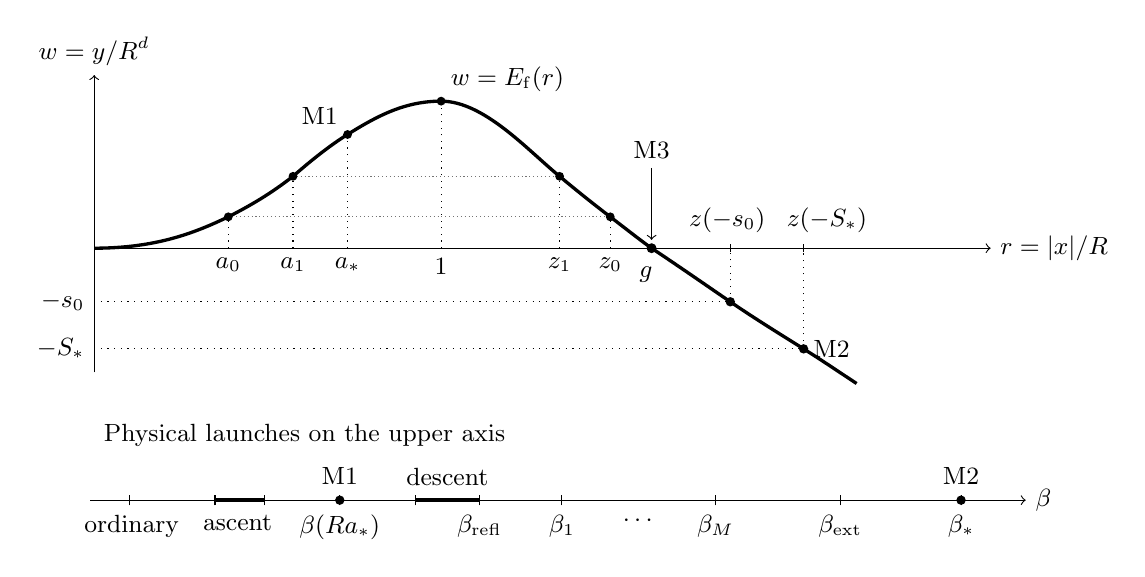
\begin{tikzpicture}[x=.99cm,y=.83cm,font=\small]
\draw[->] (0,0)--(11.5,0) node[right] {$r=|x|/R$};
\draw[->] (0,-1.9)--(0,2.65) node[above] {$w=y/R^d$};
\draw[densely dotted,black!55] (1.72,.48)--(6.62,.48)
                              (2.55,1.10)--(5.97,1.10);
\draw[very thick] (0,0) .. controls (.8,0) and (1.3,.24) .. (1.72,.48)
 .. controls (2.0,.65) and (2.26,.83) .. (2.55,1.10)
 .. controls (2.78,1.34) and (3.02,1.57) .. (3.25,1.74)
 .. controls (3.65,2.04) and (4.0,2.25) .. (4.45,2.25)
 .. controls (5.0,2.25) and (5.56,1.50) .. (5.97,1.10)
 .. controls (6.17,.90) and (6.4,.68) .. (6.62,.48)
 .. controls (6.85,.27) and (7.03,.10) .. (7.15,0)
 .. controls (7.48,-.26) and (7.89,-.60) .. (8.16,-.82)
 .. controls (8.49,-1.09) and (8.90,-1.39) .. (9.10,-1.54)
 .. controls (9.38,-1.75) and (9.60,-1.93) .. (9.78,-2.07);
\node[above right] at (4.45,2.25) {$w=E_{\rm f}(r)$};
\foreach \x/\y/\name in {1.72/.48/a_0,2.55/1.10/a_1,3.25/1.74/a_*,
                           4.45/2.25/1,5.97/1.10/z_1,6.62/.48/z_0}
  {\draw[dotted] (\x,0) node[below] {$\name$}--(\x,\y);
   \fill (\x,\y) circle (1.6pt);}
\node[above left] at (3.25,1.74) {M1};
\fill (7.15,0) circle (1.8pt) node[below=3pt,xshift=-2pt] {$g$};
\draw[->,shorten >=3pt] (7.15,1.23) node[above] {M3}--(7.15,0);
\foreach \x/\y/\level in {8.16/-.82/-s_0,9.10/-1.54/-S_*}
  {\draw[dotted] (0,\y) node[left] {$\level$}--(\x,\y)--(\x,0);
   \draw (\x,-.06)--(\x,.06);
   \fill (\x,\y) circle (1.7pt);}
\node[above=2pt] at (8.12,0) {$z(-s_0)$};
\node[above=2pt] at (9.40,0) {$z(-S_*)$};
\node[right] at (9.10,-1.54) {M2};
\begin{scope}[yshift=-3.2cm]
\node[anchor=west] at (0,1.0) {Physical launches on the upper axis};
\draw[->] (-.05,0)--(11.95,0) node[right] {$\beta$};
\foreach \x in {.45,1.55,2.18,3.15,4.12,4.94,6.00,7.97,9.57,11.12}
  \draw (\x,-.08)--(\x,.08);
\draw[line width=1.25pt] (1.55,0)--(2.18,0) (4.12,0)--(4.94,0);
\fill (3.15,0) circle (1.7pt) node[above=2pt] {M1};
\fill (11.12,0) circle (1.7pt) node[above=2pt] {M2};
\node[below] at (.48,-.08) {ordinary};
\node[below] at (1.84,-.08) {ascent};
\node[below] at (3.15,-.08) {$\beta(Ra_*)$};
\node[above] at (4.53,.08) {descent};
\node[below] at (4.94,-.08) {$\beta_{\rm refl}$};
\node[below] at (6,-.08) {$\beta_1$};
\node[below] at (7,-.08) {$\cdots$};
\node[below] at (7.97,-.08) {$\beta_M$};
\node[below] at (9.57,-.08) {$\beta_{\rm ext}$};
\node[below] at (11.12,-.08) {$\beta_*$};
\end{scope}
\end{tikzpicture}
\caption{The upper panel shows the limiting fold. The radii $a_i$ and $z_i$
lie at equal levels, $i=0,1$. M1 marks the ascending matched orbit.
M2 uses the common scaled lower intercept $-S_*$. M3 compares turns
at physical heights $0$ and $s$, both approaching $g$ in scaled
radius. The lower panel orders the actual upper launches.
The two heavy segments are the fold brackets. From $\beta_{\rm refl}$
at the plus radius $Rz_0$ to $\beta_{\rm ext}$ at scaled lower
intercept $-s_0$, the launches $\beta_i$ increase as the physical
turning heights decrease. Distances are schematic.}
\label{fig:outer-fold}
\end{figure}


One orbit closes on the ascent when the lower intercepts from a chosen
upper launch agree (M1). A second closes when the upper hits from a
chosen deep lower intercept agree (M2). This second orbit supplies a
reference on each half-plane. At a descending turn of physical height
$h$, let $\mathfrak d_\pm(h)$ be the difference between half the squared
scaled upper launch of the reference and the corresponding quantity for
the turn. The third condition is $\mathfrak d_+(0)=\mathfrak d_-(s)$
(M3). One inner odd coefficient and the two new exterior odd
coefficients realize all three equalities (\eqref{eq:miranda-box}).

Lu's exterior construction already compares ratios of gaps from a
reference on each half and pairs a finite set of heights to physical
accuracy $o(1)$ by controlling the distortion on a common terminal
section \cite[Proposition~3.3 and Lemma~3.4]{LuDegree}. His
degree-twelve construction also uses three matches and a first-order
correction for turns on the descent \cite[supplement, \S S5]{LuDegree}.
For the present profiles we compare two turns directly along the same
deep reference trajectory. In the logarithm of the ratio of their
deficits, the integral along the common part of that trajectory cancels
exactly (Lemma~\ref{lem:deficit-ratio}). What remains is a squared-slope
integral between the turns with a bounded logarithmic remainder.
On the regular descent this gives an error $O(R^{-1}+R^{2-d})$ on the
physical height scale in \eqref{eq:physical-deficit}. After (M2) and
(M3), the right turn at each prescribed $h$ and a left turn at
$h+s+o(1)$ therefore have the same launch.

The $2+6L+j$ ordinary sign changes and the $10L+2j+4$ obtained from
incoming trajectories now occur in disjoint launch intervals. The
outer fold supplies two further intervals of opposite endpoint signs
and the two simple periodic orbits just matched. Both half-returns exist
transversely throughout every interval. One regular value of an odd
coefficient already in the support gives a hyperbolic cycle in each
interval and preserves the two simple orbits
(Lemma~\ref{lem:hyperbolicity}). For one valley and $j=0$ this is
$8+14+2+2=26$ (Table~\ref{tab:ordered-returns}).

\subsection{Comparison at fixed term count and at fixed degree}\label{subsec:other-comparisons}
Table~\ref{tab:ten-comparison} compares ten-term examples with the
counts available at the same degree when all powers are allowed.

\begin{table}[!htbp]
\centering\small
\caption{Lower bounds for hyperbolic cycles with restoring force $x$.
The third column uses ten nonzero primitive terms. The last column
allows every power through the indicated degree and gives Lu's
exact-degree bounds \cite[Theorem~1.1 and supplement, Proposition~S1.2]{LuDegree}.
The sextic and trinomial rows use the odd-power extension of
Proposition~\ref{prop:outer-extension}.}
\label{tab:ten-comparison}
\begin{tabular}{@{}lrrr@{}}
\toprule
Ten-term construction & Degree & Ten terms & Degree only\\
\midrule
Full support, published \cite[Theorem~1]{DMH} & 10 & 8 & 14\\
Full support, preprint \cite[supplement, Proposition~S1.2]{LuDegree} & 10 & 14 & 14\\
Palomar sextic and four odd powers \cite{Palomar} & 13 & 10 & 22\\
Ten odd powers, averaging \cite{LMP,BCG} & 19 & 9 & 43\\
Quadratic factors, $p=2$ (Corollary~\ref{cor:short-lists}) & 22 & 16 & 53\\
Trinomial and seven odd powers \cite{CJLZ} & 23 & 10 & 57\\
Quadratic factors, $p=4$ (Corollary~\ref{cor:short-lists}) & 26 & 16 & 67\\
Cubic factors, $n_0=257$ (Corollary~\ref{cor:ten-support}) & 67088 & 26 & 234784\\
\bottomrule
\end{tabular}
\end{table}

To compare growth per term in Lu's construction, stop after $s\ge1$ separated radii, before the remaining high
odd powers are added. The three comparisons give at least $7s,3s,s$
sign changes. One linear coefficient realizes the ordinary cycles
while preserving the incoming signs, and the outer maximum closes
the incoming trajectories. The resulting primitive has degree at most
$4s+11$ and gives at least $11s+1$ hyperbolic cycles on at most $3s+9$
powers. For $k\ge12$, put $s=\lfloor(k-9)/3\rfloor$ and fill any
missing powers by hyperbolic persistence. This gives the comparison
\[
 H(k)\ge11\lfloor(k-9)/3\rfloor+1,\qquad \liminf_{k\to\infty} H(k)/k\ge11/3 .
\]
The term count for this truncation and the stronger one-radius examples
of $23$ and $24$ cycles on twelve and thirteen terms in degrees $14$
and $15$ are detailed in the electronic supplement, Section~1.1.

The increase from $11/3$ to $4$ in the guaranteed count per term
comes with a larger degree per block. In \eqref{eq:support-general}
each four-power block increases the degree by $774$, and the final degree is
$258n_0+774L+8=(387/2)k+O_{n_0}(1)$ for fixed admissible $n_0$.
At the same actual degree Lu's unrestricted theorem gives
$\lceil(7n-48)/2\rceil$ cycles for every $n\ge14$
\cite[Theorem~1.1]{LuDegree}. In degrees
$22$ and $26$ the two ten-term supports each give sixteen. With all
powers available, published constructions for $n\ge6$ give
$\lfloor(n-1)/2\rfloor+2$ \cite[Theorem~2]{DMD} and $n-2$
\cite[Theorem~1]{DMH}. The latter gives $20$ and $24$ at these degrees,
and Lu's preprint gives $53$ and $67$.
Hyperbolic persistence permits all missing powers through the given
degree to be filled.

The unsigned Palomar preprint proves an isolated-cycle lower bound
$\lfloor(n-1)/2\rfloor+4$ in exact degree $n\ge6$. Its certified sextic
has six strict return brackets \cite[Theorems~1--2 and Appendix~A]{Palomar}.
Varying its linear coefficient gives six hyperbolic cycles at nearby
coefficients by Lemma~\ref{lem:hyperbolicity}. Adjoining the powers
$7,9,11,13$ then gives the degree-thirteen entry. The degree-twenty-three
entry starts with the three hyperbolic cycles on $\{1,9,10\}$ of
Chen, Jin, Li and Zhou \cite[proof of Theorem~1.2]{CJLZ}.
Section~3 of the electronic supplement also proves this starting case.
One higher odd power at a time gives $H(k)\ge k$ for $k\ge3$
(Appendix~\ref{app:extension}).

The order of the even and odd powers matters. With the even power last,
Chen, Jin, Li and Zhou give two cycles on $\{1,3,2N\}$ for $N\ge3$
\cite[Theorem~1.1 and (2.1)]{CJLZ}. With the even power first,
Chen, Lu, Wang and Zhang consider
$F(x)=a_1x^{2N}+a_2x^{2m+1}+x^{2n+1}$, where $2\le N\le m<n$
and $a_1a_2\ne0$. Their Theorem~4 gives no limit cycles for $a_2>0$
and exactly one, hyperbolic and attracting, for $a_2<0$. In its proof
they invoke Cen and coauthors for nonexistence in the first case and
existence in the second, then establish uniqueness and hyperbolicity
in the second case \cite[Theorem~4 and \S3]{CLWZ}.

Term counts depend on the chosen coordinates. Centering the restoring force $\eps(\lambda-x)$
replaces the primitive by $[F(X+\lambda)-F(\lambda)]/\sqrt\eps$
\cite[(5)]{DMH}, so a single power can contribute every lower positive
power when $\lambda\ne0$. A different restriction appears near a
single reversible center. If the even primitive is fixed and the
coefficients of $b\ge1$ prescribed odd powers vary near zero, at most
$b-1$ isolated cycles can shrink to this center (Remark~\ref{rem:local-cyclicity}).
The cycles of Theorem~\ref{thm:main} occupy separated radial scales.

Counting monomials in both components gives $m=k+2$ in
\eqref{eq:lienard}, including $y$ and $-x$ \cite[\S2.5, Problem~8]{Gasull2021}.
With a polynomial restoring force, the examples of \'Alvarez, Coll,
De Maesschalck and Prohens \cite{ACDP} give a lower bound asymptotic
to $m\log m/(2\log 2)$ along a sequence by the count of
\cite[Theorems~1.2, 3.6 and \S5]{BCG}. For general planar fields,
Gasull and Santana obtain a quadratic lower bound from period annuli
at several centers \cite[Theorem~1 and \S3]{GS}.

\section{Half-return maps, inward graphs, tail balance, and hyperbolicity}\label{sec:toolkit}


The reflected half-returns satisfy the variational identities used
for trinomials by Chen, Jin, Li and Zhou. Their running-minimum
estimate controls contraction along an inward leg
\cite[Proposition~2.2, (3.5)--(3.7) and (3.17)--(3.19)]{CJLZ}.
We shall need these estimates both for finite turns and for inward
graphs with a prescribed limiting ordinate at infinity.


\subsection{Reflection, Filippov potential coordinates, and variational identities}\label{subsec:half-returns}
Given $F$ as in \eqref{eq:collected}, define the two half-profiles $P_+(r)=F(r)$ and $P_-(r)=F(-r)$
for $r\ge 0$. On the right half-plane $\{x\ge 0\}$ with $r=x$ and forward time $t$, and on the left
half-plane $\{x\le 0\}$ under the reflection $r=-x\ge 0$ and time reversal $\tilde{t}=-t$, system
\eqref{eq:lienard} takes the common form
\begin{equation}\label{eq:half-system}
  \dot{r} = y - P_\sigma(r), \qquad \dot{y} = -r \qquad (r\ge 0,\ \sigma\in\{+,-\}).
\end{equation}

Throughout $\{r>0\}$ one has $\dot{y}=-r<0$, so the ordinate $y$ decreases strictly along every
trajectory segment in $\{r>0\}$. Filippov introduced the potential separately on the two half-axes
\cite[pp.~171--172, (2)--(6)]{Filippov}. 
The potential coordinate $u=r^2/2\ge 0$
expresses each half-trajectory in $\{r>0\}$ as a single-valued smooth graph $u=u_\sigma(y)$ satisfying
\begin{equation}\label{eq:filippov}
  \frac{\dd u_\sigma}{\dd y} = \frac{r\dot{r}}{\dot{y}} = P_\sigma(\sqrt{2u_\sigma}) - y.
\end{equation}

At any interior critical point of $u_\sigma(y)$, where $y=P_\sigma(\sqrt{2u_\sigma})$, differentiating
\eqref{eq:filippov} with respect to $y$ yields $u_{\sigma,yy}=-1<0$. Consequently, each half-arc in
$\{r>0\}$ possesses at most one stationary radius, which is necessarily a strict global maximum
$r=t_\sigma>0$ called its \emph{turn}.


For $\beta>0$, launch the trajectory of \eqref{eq:half-system} from $(0,\beta)$ into $\{r>0\}$.
Whenever it first returns transversely to $\{r=0\}$ at a finite negative ordinate, denote that
ordinate by $b_\sigma(\beta)<0$, and define the half-return displacement
\[
  \oscD(\beta) = b_+(\beta) - b_-(\beta)
\]
on the common open domain of transverse returns. To analyze multiscale limits uniformly, given radial
and ordinate scales $\Lambda,M>0$ we set $\eps=(\Lambda/M)^2$, $w=y/M$, $\tilde{u}=u/\Lambda^2=(r/\Lambda)^2/2$, and
$\phi_\sigma(\tilde{u})=M^{-1}P_\sigma(\Lambda\sqrt{2\tilde{u}})$. For a half-arc turning at $\tilde{u}=T>0$
(physical radius $\Lambda\sqrt{2T}$) that meets both vertical half-axes transversely at $(0,Mw_o(0))$
($w_o(0)>0$) and $(0,Mw_i(0))$ ($w_i(0)<0$), its outward leg $w_o(\tilde{u})$ and inward leg
$w_i(\tilde{u})$ on $[0,T]$ solve
\begin{equation}\label{eq:scaled-legs}
  \frac{\dd w}{\dd\tilde{u}} = \frac{\eps}{\phi_\sigma(\tilde{u})-w}, \qquad w_o(\tilde{u}) >
  \phi_\sigma(\tilde{u}) > w_i(\tilde{u}) \quad (0<\tilde{u}<T), \qquad w_o(T)=w_i(T)=\phi_\sigma(T).
\end{equation}
Define the half-squared scaled axis intercepts $X_\sigma(T)=\frac{1}{2}w_o(0)^2$ and
$Y_\sigma(T)=\frac{1}{2}w_i(0)^2$, together with the suffix running extrema on $[0,T]$:
\begin{equation}\label{eq:running-extrema}
  m_{\sigma,T}(\tilde{u}) = \max_{s\in[\tilde{u},T]} \phi_\sigma(s), \qquad l_{\sigma,T}(\tilde{u}) =
  \min_{s\in[\tilde{u},T]} \phi_\sigma(s).
\end{equation}

\begin{lemma}[Single crossing, variational derivatives, and running-extremum bounds]\label{lem:variational}
Let $F$ be a real polynomial with $F(0)=0$.
\begin{enumerate}
  \item[\textup{(i)}] Every periodic orbit of \eqref{eq:lienard} surrounds $(0,0)$ and intersects each
  of the rays $\{x=0,y>0\}$ and $\{x=0,y<0\}$ transversely in a single point. Periodic orbits of
  \eqref{eq:lienard} stand in bijection with zeros $\beta>0$ of $\oscD(\beta)=b_+(\beta)-b_-(\beta)$,
  and at any matched orbit $\oscD(\beta_*)=0$ the first-return map $\Pi(\beta)=b_-^{-1}(b_+(\beta))$
  has Floquet multiplier $\Pi'(\beta_*)=b_+'(\beta_*)/b_-'(\beta_*)$.
  \item[\textup{(ii)}] On the domain of transverse returns, $b_\sigma(\beta)<0$ is real analytic and strictly decreasing in $\beta$, with
  \begin{equation}\label{eq:b-deriv}
    b_\sigma'(\beta) = \frac{\beta}{b_\sigma(\beta)} e^{-J_\sigma(\beta)}, \qquad J_\sigma(\beta) =
    \int_{\mathrm{arc}} P_\sigma'(r(t))\dd t = \int_{b_\sigma(\beta)}^{\beta}
    \frac{P_\sigma'(\sqrt{2u_\sigma(y)})}{\sqrt{2u_\sigma(y)}}\dd y.
  \end{equation}
  At a matched periodic orbit $\oscD(\beta_*)=0$, one has
  $\Pi'(\beta_*)=\exp(J_-(\beta_*)-J_+(\beta_*))$ and $\sgn(\Pi'(\beta_*)-1)=-\sgn\oscD'(\beta_*)$.
  Furthermore, if $P_{\sigma,\mu}(r)=P_{\sigma,0}(r)+\mu\,\partial_\mu P_{\sigma,0}(r)+o(\mu)$ varies
  smoothly with a parameter $\mu$ at fixed $\beta$, then
  \begin{equation}\label{eq:b-param}
    \partial_\mu b_\sigma(\beta,\mu) = -\frac{1}{b_\sigma(\beta,\mu)}
    \int_{b_\sigma(\beta,\mu)}^{\beta} \exp\!\left(-\int_{b_\sigma(\beta,\mu)}^{y}
    \frac{P_{\sigma,\mu}'(\sqrt{2u_\sigma(v)})}{\sqrt{2u_\sigma(v)}}\dd v\right) \partial_\mu
    P_{\sigma,\mu}(\sqrt{2u_\sigma(y)})\dd y.
  \end{equation}
  For two polynomial half-profiles $P_1,P_2$ vanishing at zero, fix a common
  launch $\beta>0$ for which both half-arcs return transversely to
  $\{r=0,y<0\}$. If $P_2\ge P_1$ on the union of their radial ranges,
  with strict inequality on a nonempty open radial interval traversed
  by both arcs, then $b_{P_2}(\beta)>b_{P_1}(\beta)$.
  \item[\textup{(iii)}] For any turn $T>0$ with transverse axis hits in the scaled coordinates
  \eqref{eq:scaled-legs}, $X_\sigma(T)$ and $Y_\sigma(T)$ increase strictly with $T$ and satisfy
  \begin{equation}\label{eq:turn-derivs}
    X_\sigma'(T) = \eps e^{J_{o,\sigma}(T)}, \quad Y_\sigma'(T) = \eps e^{-J_{i,\sigma}(T)}, \quad
    -\eps J_{o,\sigma}(T) = \int_0^T \phi_\sigma'\dd w_o, \quad \eps J_{i,\sigma}(T) = \int_0^T
    \phi_\sigma'\dd w_i,
  \end{equation}
  where $J_\sigma = J_{o,\sigma}+J_{i,\sigma}$. Moreover, for every $\tilde{u}\in[0,T]$,
  \begin{equation}\label{eq:envelope-bounds}
    0 \le w_o(\tilde{u}) - m_{\sigma,T}(\tilde{u}) \le \sqrt{2\eps(T-\tilde{u})}, \qquad 0 \le
    l_{\sigma,T}(\tilde{u}) - w_i(\tilde{u}) \le \sqrt{2\eps(T-\tilde{u})}.
  \end{equation}
\end{enumerate}
\end{lemma}


\begin{proof}
(i) Because $\dot{y}=-x$ vanishes only on $\{x=0\}$ and $(0,0)$ is the sole equilibrium of
\eqref{eq:lienard} (as $y-F(0)=y=0$ on $\{x=0\}$), no periodic orbit can lie in $\{x\ge 0\}$ or
$\{x\le 0\}$, and by index theory every periodic orbit $\Gamma$ is a simple closed Jordan curve
enclosing $(0,0)$. Along $\{x=0,y>0\}$ one has $\dot{x}=y>0$, so $\Gamma$ crosses $\{x=0,y>0\}$
transversely from left to right at every intersection. The signed intersection number with this ray is
the winding number of
the Jordan curve about the origin, of absolute value one. All crossings
have the same sign, so there is exactly one. On the negative ray all
crossings again have the same sign. Reversing time on $\{x\le 0\}$ gives $\oscD(\beta)=0$ as the exact
closure condition and $\Pi=b_-^{-1}\circ b_+$.

(ii) Near a transverse axis hit $y_0\ne 0$ ($\beta>0$ or $b_\sigma<0$), the planar trajectory
satisfies $y(r)=y_0-r^2/(2y_0)+O(r^3)$, hence $u_\sigma(y)=-y_0(y-y_0)+O(|y-y_0|^{3/2})$ and
$u_{\sigma,y}(y_0)=-y_0\ne 0$. Since $F(0)=0$, the coefficient
$g_\sigma(y)=P_\sigma'(\sqrt{2u_\sigma(y)})/\sqrt{2u_\sigma(y)}$ is
$O(u_\sigma(y)^{-1/2})=O(|y-y_0|^{-1/2})$, which is integrable at both endpoints $b_\sigma$ and
$\beta$. Differentiating \eqref{eq:filippov} and $u_\sigma(\beta,\beta,\mu)=0$ with respect to
$(\beta,\mu)$ gives the linear variational equation $\partial_y(\delta u_\sigma)=g_\sigma(y)\,\delta
u_\sigma + \partial_\mu P_{\sigma,\mu}(\sqrt{2u_\sigma})\,\delta\mu$ with boundary value $\delta
u_\sigma(\beta)=\beta\,\delta\beta$ (since $u_{\sigma,y}(\beta)\,\delta\beta+\delta u_\sigma(\beta)=0$
and $u_{\sigma,y}(\beta)=-\beta$). Integrating from $\beta$ down to $b_\sigma$ yields
\[
  \delta u_\sigma(b_\sigma) = \beta e^{-J_\sigma(\beta)}\,\delta\beta - \left(\int_{b_\sigma}^\beta
  e^{-\int_{b_\sigma}^y g_\sigma(v)\dd v}\,\partial_\mu P_{\sigma,\mu}(\sqrt{2u_\sigma(y)})\dd
  y\right)\delta\mu,
\]
where $\int_{b_\sigma}^\beta g_\sigma(y)\dd y=\int_{\mathrm{arc}}P_\sigma'(r(t))\dd t=J_\sigma(\beta)$
via $\dd y=-r\dd t=-\sqrt{2u_\sigma}\dd t$. Differentiating
$u_\sigma(b_\sigma(\beta,\mu),\beta,\mu)=0$ gives $-b_\sigma\,\delta b_\sigma+\delta
u_\sigma(b_\sigma)=0$, proving \eqref{eq:b-deriv} and \eqref{eq:b-param}. Because $b_-'(\beta_*)<0$,
$\Pi'(\beta_*)-1=\oscD'(\beta_*)/b_-'(\beta_*)$ has sign $-\sgn\oscD'(\beta_*)$. For the finite comparison write
$b_i=b_{P_i}(\beta)$, $r_i=\sqrt{2u_i}$ and compare the two graphs
at common ordinates $\max(b_1,b_2)\le y\le\beta$. Their difference
$d=u_2-u_1$ solves
\[
 d'=g(y)d+P_2(r_1)-P_1(r_1),\qquad d(\beta)=0,
\]
where $g$ is the divided difference of $u\mapsto P_2(\sqrt{2u})$.
In the interior $|g|\le 2\sup|P_2'|/(r_1+r_2)$, with the supremum
over the two radial ranges. The transverse expansions above make
this bound integrable even at a shared hit. Integrating backwards
gives $d\le0$. If $b_2\le b_1$, the common ordinate interval contains
the whole first excursion. There the forcing is positive on an open
set, hence $d(b_1)<0$, whereas $d(b_1)=u_2(b_1)\ge0$. Thus $b_2>b_1$.
Two returning arcs of the same
half-field enclose a compact strip with the axis. Intermediate launches
return in that strip by uniqueness and monotonicity of $y$.

(iii) In scaled variables \eqref{eq:scaled-legs}, view $\tilde{u}=\tilde{u}_o(w,T)$ on
$[\phi_\sigma(T),w_o(0)]$ as solving $\eps\,\partial_w\tilde{u}_o=\phi_\sigma(\tilde{u}_o)-w$ with
$\tilde{u}_o(\phi_\sigma(T),T)=T$. Since $\partial_w\tilde{u}_o(\phi_\sigma(T),T)=0$, differentiating
at $w=\phi_\sigma(T)$ gives $(\partial_T\tilde{u}_o)(\phi_\sigma(T),T)=1$. Integrating
$\eps\,\partial_w(\partial_T\tilde{u}_o)=\phi_\sigma'(\tilde{u}_o)\,\partial_T\tilde{u}_o$ from
$\phi_\sigma(T)$ to $w_o(0)$ gives
\[
  (\partial_T\tilde{u}_o)\bigl(w_o(0),T\bigr) =
  \exp\!\left(\frac{1}{\eps}\int_{\phi_\sigma(T)}^{w_o(0)}\phi_\sigma'\bigl(\tilde{u}_o(w)\bigr)\dd
  w\right) = e^{J_{o,\sigma}(T)},
\]
where $-\eps J_{o,\sigma}(T)=\int_0^T\phi_\sigma'(\tilde{u})\dd w_o(\tilde{u})$. Differentiating
$\tilde{u}_o(w_o(0,T),T)=0$ gives $-(w_o(0)/\eps)\partial_T
w_o(0)+(\partial_T\tilde{u}_o)(w_o(0),T)=0$, so $X_\sigma'(T)=w_o(0)\partial_T w_o(0)=\eps
e^{J_{o,\sigma}(T)}$. The analogous integration on $[w_i(0),\phi_\sigma(T)]$ gives $Y_\sigma'(T)=\eps
e^{-J_{i,\sigma}(T)}$.

Finally, fix $\tilde{u}_0\in[0,T]$ and put $M_0=m_{\sigma,T}(\tilde{u}_0)$. Since $\dd
w_o/\dd\tilde{u}<0$ and $w_o(s)>\phi_\sigma(s)$ on $(0,T)$ with $w_o(T)=\phi_\sigma(T)\le M_0$, we
have $w_o(\tilde{u}_0)\ge M_0$. If $w_o(\tilde{u}_0)>M_0$, let $s_*\in(\tilde{u}_0,T]$ be the first
point where $w_o(s_*)=M_0$. On $[\tilde{u}_0,s_*)$, $w_o(s)>M_0\ge\phi_\sigma(s)$, whence
\[
  \frac{\dd}{\dd s}\bigl(w_o(s)-M_0\bigr)^2 = -2\eps\,\frac{w_o(s)-M_0}{w_o(s)-\phi_\sigma(s)} \ge -2\eps.
\]
Integrating across $[\tilde{u}_0,s_*]$ yields $(w_o(\tilde{u}_0)-M_0)^2\le 2\eps(s_*-\tilde{u}_0)\le
2\eps(T-\tilde{u}_0)$. Applying the same argument to $-w_i$ and $-\phi_\sigma$ proves the second
estimate in \eqref{eq:envelope-bounds}.
\end{proof}


\subsection{Coercive tail limits, tail balancing, and inward graphs from infinity}\label{subsec:tail-inward}

For even degree $d>2$ and positive leading coefficient, both half-profiles
grow at least as fast as a positive multiple of $r^d$. A returning
half-arc then determines a finite limiting lower intercept $\ell_\sigma$
as the launch height grows. When the primitive starts in degree at least
two, one can also prescribe a finite ordinate at infinity and integrate
inward. The resulting intercept $G_\sigma(h)$ varies strictly with this
ordinate. Both assertions use the integrability of $r^{1-d}$ at infinity.


\begin{lemma}[Tail limits, strict odd monotonicity, and inward graphs]\label{lem:tail-inward}
Let $P$ be a real polynomial with $P(0)=0$ such that $P_\sigma(r)=P(\sigma r)$ satisfies
$P_\sigma(r)\ge c_0 r^d$ for all $r\ge K_0$, where $d>2$ and $c_0,K_0>0$. Suppose that either
$b_\sigma(\beta_0)<0$ exists transversely at some $\beta_0>0$, or $\min\supp(P)\ge 2$.
\begin{enumerate}
  \item[\textup{(i)}] Transverse returns $b_\sigma(\beta)<0$ exist for all $\beta\ge\beta_0$ (and for
  all $\beta>0$ when $\min\supp(P)\ge 2$), and the limit
  $\ell_\sigma(P)=\lim_{\beta\to+\infty}b_\sigma(\beta)$ is finite and strictly negative.
  \item[\textup{(ii)}] If polynomials $P_n$ with $P_n(0)=0$ converge to $P$ in $C^1$ on compact
  subsets of $\mathbb{R}$ and satisfy the uniform tail barrier $P_n(\sigma r)\ge c_0 r^d$ for all
  $r\ge K_0$, then $b_{P_n(\sigma\cdot)}(\beta_n)\to\ell_\sigma(P)$ whenever $\beta_n\to+\infty$; in
  particular, $\ell_\sigma(P_n)\to\ell_\sigma(P)$.
  The same conclusion for the finite intercepts holds under a truncated
  bound. Assume $P_n(\sigma r)\ge c_0r^d$ only for $K_0\le r\le R_n$,
  with $R_n\to\infty$. Let an actual half-arc have upper hit $\beta_n\to\infty$,
  turn $t_n\le R_n$ and transverse lower hit $b_n<0$. Then $b_n\to\ell_\sigma(P)$.
  Here the terminal ordinate of the inward leg is $P_n(\sigma t_n)$.
  The rotation argument in (i) supplies both hits from a prescribed
  finite turn when $\min\supp(P_n)\ge2$.
  \item[\textup{(iii)}] For every integer $1\le m<d$, the map $\lambda\mapsto\ell_\sigma(P+\lambda
  x^m)$ is continuous and strictly increasing (when $\sigma=+$) or strictly decreasing (when
  $\sigma=-$ and $m$ is odd) on any interval of $\lambda$ where transverse returns exist.
  Consequently, for odd $1\le m<d$, the tail gap $\Delta(P+\lambda x^m)=\ell_+(P+\lambda
  x^m)-\ell_-(P+\lambda x^m)$ increases strictly with $\lambda$.
  \item[\textup{(iv)}] If $\min\supp(P)\ge 2$, then for every $h\in\mathbb{R}$ there exists a unique
  solution $y_{\sigma,h}\in C^1([0,\infty))$ of the inward graph equation
  \begin{equation}\label{eq:inward-ode}
    y'(r) = \frac{r}{P_\sigma(r) - y(r)}, \qquad y(r) < P_\sigma(r) \quad (r\ge 0), \qquad \lim_{r\to+\infty} y(r) = h.
  \end{equation}
  Its axis intercept $G_\sigma(h)=y_{\sigma,h}(0)$ is smooth and strictly increasing on $\mathbb{R}$,
  satisfies $G_\sigma(h)<\ell_\sigma(P)$ for all $h\in\mathbb{R}$,
  $\lim_{h\to+\infty}G_\sigma(h)=\ell_\sigma(P)$, and $\lim_{h\to-\infty}(G_\sigma(h)-h)=0$. Moreover,
  under the global barrier hypotheses of \textup{(ii)} with $\min\supp(P_n)\ge 2$, one has
  $G_{\sigma,P_n}(h)\to G_{\sigma,P}(h)$ uniformly on compact $h$-intervals.
\end{enumerate}
\end{lemma}


\begin{proof}
(i) When $\min\supp(P)\ge 2$, the linearization of \eqref{eq:half-system} at $(0,0)$ has polar angular
speed $-1+O(|(r,y)|)$, bounded away from zero near $(0,0)$, so no half-orbit can approach $(0,0)$ from
$\{r>0\}$. Starting from any turn $(t,P_\sigma(t))$ ($t>0$), $r$ decreases away from $t$ in both time
directions, cannot stall at a positive radius (since $\dot{y}=-r$), stays bounded in $y$ by the envelope estimate
\eqref{eq:envelope-bounds} on each partial leg, and avoids $(0,0)$, hence hits both $\{r=0,y>0\}$ and $\{r=0,y<0\}$
transversely. This argument from a finite turn needs no assumption at
infinity and also applies to the terminal folds below. When $b_\sigma(\beta_0)<0$ is assumed, for every $\beta>\beta_0$ coercivity
$P_\sigma(r)>\beta$ forces a finite turn, and the trajectory from $(0,\beta_0)$ separates $(0,0)$ from
the inward leg from $(0,\beta)$, ensuring a transverse return $b_\sigma(\beta)<b_\sigma(\beta_0)<0$.

On the inward leg $Y'(r)=r/(P_\sigma(r)-Y(r))$ ($Y<P_\sigma$), choose $A_1\ge K_0$ so large that the
barrier $B(r)=\frac{1}{2}c_0 r^d$ satisfies $B'(r)=\frac{d}{2}c_0 r^{d-1} > \frac{2}{c_0}r^{1-d}$ for
all $r\ge A_1$ (using $d>2$). Choose $\alpha_*<0$ so negative that the solution $Y_*(r)$ of
$Y'=r/(P_\sigma(r)-Y)$ with $Y_*(0)=\alpha_*$ stays below $\min_{[0,A_1]}P_\sigma-1$ on $[0,A_1]$ and
satisfies $Y_*(A_1)<B(A_1)$. On $[A_1,\infty)$, at any hypothetical first contact $Y_*(r)=B(r)$ one
would have $Y_*'(r)=r/(P_\sigma(r)-\frac{1}{2}c_0 r^d)\le 2r^{1-d}/c_0 < B'(r)$, a contradiction.
Hence $Y_*(r)<B(r)<P_\sigma(r)$ for $r\ge A_1$, and $Y_*<P_\sigma$ also on $[0,A_1]$, so $Y_*$ never
turns. Scalar comparison of $Y'=r/(P_\sigma(r)-Y)$ shows $b_\sigma(\beta)>\alpha_*$ for all $\beta$,
and monotonicity gives $\ell_\sigma(P)\in[\alpha_*,b_\sigma(\beta_0)]$.

(ii) Fix $\alpha<\ell_\sigma(P)$ and put $\delta=\ell_\sigma(P)-\alpha>0$. As $\beta\to+\infty$, the
turns $t(\beta)$ of returning orbits diverge by \eqref{eq:envelope-bounds}, and their inward legs
$Y_\beta^-(r)$ satisfy $Y_\beta^-(0)=b_\sigma(\beta)>\ell_\sigma(P)=\alpha+\delta$. Since vertical
gaps between solutions of $Y'=r/(P_\sigma(r)-Y)$ are nondecreasing in $r$ (as
$\partial_Y[r/(P_\sigma-Y)]>0$), the solution $Y_\alpha$ from $Y_\alpha(0)=\alpha$ exists for all
$r\ge 0$ and satisfies $P_\sigma(r)-Y_\alpha(r)>Y_\beta^-(r)-Y_\alpha(r)\ge \delta$, whence
$Y_\alpha'(r)\le r/\delta$ and $Y_\alpha(r)\le \alpha+r^2/(2\delta)$. Choose $A_1\ge K_0$ as above
with $\alpha+A_1^2/(2\delta)<\frac{1}{2}c_0 A_1^d$. By compact $C^1$ convergence on $[0,A_1]$, for all
large $n$ the solution $Y_{\alpha,n}$ from $\alpha$ remains strictly below
$P_n(\sigma r)$ on $[0,A_1]$ and satisfies $Y_{\alpha,n}(A_1)<B(A_1)$. The first-contact argument in (i) extends it
strictly below $B$ up to $R_n$ in the truncated case. The turns
$t_n$ tend to infinity: on a bounded radial interval the upper-envelope
bound and compact convergence bound the upper hit. Thus
\[
 Y_{\alpha,n}(t_n)<B(t_n)<P_n(\sigma t_n)=Y_n^-(t_n).
\]
Ordering just before the turn and uniqueness back to the axis give
$b_n>\alpha$. For the reverse bound fix a returning launch $B_0>\beta_0$
of the limit profile. Its transverse arc persists on a compact set for
$P_n$, with $b_{P_n(\sigma\cdot)}(B_0)\to b_\sigma(B_0)$.
The arc from $\beta_n>B_0$ cannot cross this inner arc, so its lower
hit lies below that from $B_0$. Taking the lower and upper limits, then
$\alpha\uparrow\ell_\sigma(P)$ and $B_0\to\infty$, proves the claim.
For the global barrier all sufficiently high launches turn and return,
by (i) and persistence of the fixed inner arc. Choosing those launches
arbitrarily far out also gives convergence of the limiting intercepts.
In the truncated assertion the comparison at $t_n$ uses the turning
ordinate itself. Prescribing a bounded ordinate $h$ at a distant cut
instead leads to the incoming graph of (iv).

(iii) Since $1\le m<d$, $(P+\lambda x^m)(\sigma r)\ge \frac{1}{2}c_0 r^d$ holds on $[K_1,\infty)$
locally uniformly in $\lambda$, so continuity of $\lambda\mapsto\ell_\sigma(P+\lambda x^m)$ follows
from~(ii). Take $\lambda_2>\lambda_1$ with $\sigma=+$, so $Q_2(r)=P(r)+\lambda_2 r^m > P(r)+\lambda_1
r^m = Q_1(r)$ for all $r>0$. For every sufficiently large common
launch both returns exist by (i). Lemma~\ref{lem:variational}(ii) gives $b_{Q_2}(\beta)>b_{Q_1}(\beta)$,
hence $\ell_+(Q_2)\ge \ell_+(Q_1)$. Chen, Jin, Li and Zhou prove the
strict order for their trinomial profiles by a uniform parameter
variation \cite[Lemma~2.9, (2.41)--(2.45)]{CJLZ}. Here it follows
by comparing the two limiting graphs on a fixed short interval. Suppose toward a contradiction that
$\ell_+(Q_2)=\ell_+(Q_1)=\ell<0$. Choose $r_0>0$ so small that $\min_{[0,r_0]} Q_i \ge \ell/2 > \ell$
for $i=1,2$. On $[0,r_0]$, the ODEs $Y'=r/(Q_i(r)-Y)$ are smooth and uniformly Lipschitz on $\{Y\le
3\ell/4\}$. Since $b_{Q_i}(\beta)\downarrow\ell$, continuous dependence on $[0,r_0]$ implies
$Y_{i,\beta}^-(r)\to Y_i(r)$ uniformly on $[0,r_0]$ as $\beta\to+\infty$, where $Y_i$ solves
$Y_i'=r/(Q_i-Y_i)$ with $Y_i(0)=\ell$. Because $Q_2(r)>Q_1(r)$ on $(0,r_0]$ and $Y_1(0)=Y_2(0)=\ell$,
differential comparison gives $Y_2(r_0)<Y_1(r_0)$. Yet at every large finite $\beta$, integrating
\eqref{eq:filippov} downward from $u_{1,\beta}(\beta)=u_{2,\beta}(\beta)=0$ shows
$u_{2,\beta}(y)<u_{1,\beta}(y)$ for all $y\in[b_{Q_2}(\beta),\beta)$; because the inward legs
$Y_{i,\beta}^-(r)$ increase strictly with $r$, lying strictly inside the $Q_1$-arc means
$Y_{2,\beta}^-(r_0)>Y_{1,\beta}^-(r_0)$. Passing to $\beta\to+\infty$ yields $Y_2(r_0)\ge Y_1(r_0)$, a
contradiction.

(iv) Fix $h\in\mathbb{R}$ and choose $K_h\ge K_0$ such that $P_\sigma(r)\ge c_0 r^d >
\max(h,0)+2|h|+2$ for all $r\ge K_h$. For each $K\ge K_h$, let $y_K(r)$ solve
$y'(r)=r/(P_\sigma(r)-y(r))$ backwards on $[0,K]$ from $y_K(K)=h$. Because $\min\supp(P)\ge 2$, the
ordinary returning arc turning at $(K,P_\sigma(K))$ has an inward leg $Y_{(K)}^-(r)$ defined on
$[0,K]$ with $Y_{(K)}^-(r)<P_\sigma(r)$ on $[0,K)$ and $Y_{(K)}^-(K)=P_\sigma(K)>h=y_K(K)$. By
uniqueness for the scalar ODE on $[0,K]$, $y_K(r)<Y_{(K)}^-(r)<P_\sigma(r)$ throughout $[0,K]$ and
$y_K'(r)>0$, so $y_K(r)\le h$ on $[0,K]$. For $K_2>K_1\ge K_h$,
\[
  0 \le h - y_{K_2}(K_1) = \int_{K_1}^{K_2} \frac{r\dd r}{P_\sigma(r)-y_{K_2}(r)} \le
  \int_{K_1}^\infty \frac{r\dd r}{P_\sigma(r)-h} \xrightarrow{K_1\to\infty} 0.
\]
For any two solutions $y_a,y_b<P_\sigma$ on $[0,K_1]$, $\frac{\dd}{\dd
r}|y_a(r)-y_b(r)|=\frac{r|y_a-y_b|}{(P_\sigma-y_a)(P_\sigma-y_b)}>0$, so backward integration from
$K_1$ to $0$ strictly contracts $|y_a-y_b|$. Hence $\{y_K\}$ is uniformly Cauchy on $[0,K_1]$ for
every $K_1\ge K_h$, converging to a solution $y_{\sigma,h}$ of \eqref{eq:inward-ode}. Uniqueness
follows because any two solutions with limit $h$ have $|y_1(r)-y_2(r)|$ nondecreasing on $[0,\infty)$
and tending to $0$ at $+\infty$.

Comparing $y_{\sigma,h}$ on $[0,t(\beta)]$ with $Y_\beta^-$ for $P_\sigma(t(\beta))>h$ gives
$G_\sigma(h)<b_\sigma(\beta)$, so $G_\sigma(h)\le \ell_\sigma(P)$; strict monotonicity of $h\mapsto
G_\sigma(h)$ (two graphs of distinct limiting heights are strictly ordered at a sufficiently large
finite cut, and uniqueness preserves strict order to the axis) then yields
$G_\sigma(h)<G_\sigma(h+1)\le \ell_\sigma(P)$. Conversely, in part~(ii) we showed that for every
$\alpha<\ell_\sigma(P)$, the inward solution $Y_\alpha$ from $Y_\alpha(0)=\alpha$ satisfies
$Y_\alpha(r)\le\alpha+r^2/(2\delta)<\frac{1}{2}c_0 r^d$ for large $r$, whence
$Y_\alpha'(r)=O(r^{1-d})$ integrates to a finite limit $h(\alpha)=\lim_{r\to\infty}Y_\alpha(r)$, so
$G_\sigma(h(\alpha))=\alpha$ and $\lim_{h\to+\infty}G_\sigma(h)=\ell_\sigma(P)$. For $h<M_*-1$ where
$M_*=\min_{r\ge 0}P_\sigma(r)$, $0\le h-G_\sigma(h)=\int_0^\infty\frac{r\dd
r}{P_\sigma(r)-y_{\sigma,h}(r)}\le \int_0^\infty\frac{r\dd r}{P_\sigma(r)-h}\to 0$ as $h\to-\infty$ by
dominated convergence. Differentiation at a finite cutoff followed by passage to the limit gives
$G_\sigma'(h)=\exp[-\int_0^\infty r(P_\sigma-y_{\sigma,h})^{-2}\dd r]>0$.
The differentiated tail converges uniformly for $h$ in a compact interval
by the same polynomial lower bound; higher derivatives follow by successive
differentiation of the graph equation. Finally, under uniform coercivity $P_n(\sigma r)\ge c_0 r^d$
($r\ge K_0$), the tail loss $\int_{K_1}^\infty r/(c_0 r^d-h)\dd r$ is uniform on compact $h$-intervals
and backward contraction transfers compact convergence on $[0,K_1]$ to $G_{\sigma,P_n}(h)\to
G_{\sigma,P}(h)$.
\end{proof}


\subsection{Simultaneous hyperbolicity on a fixed support}\label{subsec:hyperbolicity}

De Maesschalck and Dumortier observed that each odd coefficient of
the classical primitive is a rotation parameter \cite[pp.~2163--2164]{DMD}.
Indeed, for $X_\mu=(y-F(x)-\mu x^m,-x)$ with $m$ odd,
$\det(X_\mu,\partial_\mu X_\mu)=-x^{m+1}$ has one sign off the axis.
Cai, Chen, Jin and Lu use a linear rotation and a regular value to
obtain simple fixed points simultaneously for a continuous piecewise
linear primitive \cite[proof of Theorem~1.1 in \S2]{CCJL}. Lu uses
the linear coefficient for polynomial returns
\cite[Proposition~2.4(i)]{LuDegree}. In our fixed support we can use
any odd exponent already present. Formula~\eqref{eq:b-param} gives
strict parameter derivatives of opposite signs for the two half-returns.
This allows all selected brackets to be regularized with a single change
of coefficient.

\begin{lemma}[Single-field regularization and openness]
Let\label{lem:hyperbolicity} $F_0(x)=\sum_{i=1}^k a_i x^{m_i}$ ($a_i\ne 0$) contain an odd exponent $m_*=m_{i_0}\in\supp(F_0)$,
and set $F_\mu(x)=F_0(x)+\mu x^{m_*}$. Suppose that at $\mu=0$:
\begin{enumerate}
  \item[\textup{(a)}] $I_1,\dots,I_N\subset(0,\infty)$ are pairwise disjoint compact intervals
  throughout which both transverse half-returns $b_{\pm,0}(\beta)<0$ exist, and
  $\oscD_0(\beta)=b_{+,0}(\beta)-b_{-,0}(\beta)$ has opposite strict signs at the two endpoints of
  each $I_r$ ($1\le r\le N$);
  \item[\textup{(b)}] $\beta_1^*,\dots,\beta_M^*\in(0,\infty)\setminus\bigcup_{r=1}^N I_r$ are
  distinct hyperbolic periodic-orbit intercepts ($\oscD_0(\beta_s^*)=0$, $\oscD_0'(\beta_s^*)\ne 0$).
\end{enumerate}
Then there exists $\mu_0\in(0,|a_{i_0}|)$ such that for Lebesgue-almost-every $\mu\in(-\mu_0,\mu_0)$,
the polynomial $F_\mu$ satisfies $\supp(F_\mu)=\supp(F_0)$ and system \eqref{eq:lienard} for $F=F_\mu$
admits at least $N+M$ distinct hyperbolic limit cycles. Consequently, the set of coefficient vectors
on $\supp(F_0)$ realizing at least $N+M$ distinct hyperbolic limit cycles has nonempty interior in
$(\mathbb{R}\setminus\{0\})^k$.
\end{lemma}


\begin{proof}
Choose disjoint compact intervals $J_1,\dots,J_M\subset(0,\infty)\setminus\bigcup_{r=1}^N I_r$ with
$\beta_s^*\in\operatorname{int}(J_s)$ on which $\oscD_0'\ne 0$ and $\oscD_0$ has opposite strict signs
at $\partial J_s$. By real-analytic dependence of transverse half-returns and the implicit function
theorem on $J_1,\dots,J_M$, there exists $\mu_0\in(0,|a_{i_0}|)$ such that for all
$\mu\in(-\mu_0,\mu_0)$: (i) $a_{i_0}+\mu\ne 0$, so $\supp(F_\mu)=\supp(F_0)$; (ii)
$b_{\pm,\mu}(\beta)<0$ remain well-defined and real analytic on an open neighborhood $U$ of
$\bigl(\bigcup_{r=1}^N I_r\bigr)\cup\bigl(\bigcup_{s=1}^M J_s\bigr)$; (iii)
$\oscD_\mu(\beta)=b_{+,\mu}(\beta)-b_{-,\mu}(\beta)$ retains its strict opposite endpoint signs on
every $I_r$; and (iv) each $J_s$ contains a unique zero $\beta_s^*(\mu)$ of $\oscD_\mu$ with
$\oscD_\mu'(\beta_s^*(\mu))\ne 0$.

Because $m_*$ is odd, $P_{\sigma,\mu}(r)=P_{\sigma,0}(r)+\sigma\mu r^{m_*}$ has $\partial_\mu
P_{\sigma,\mu}(r)=\sigma r^{m_*}$. By \eqref{eq:b-param} in Lemma~\ref{lem:variational}(ii), since
$-b_{\sigma,\mu}>0$ and $u_\sigma(y)>0$ on $(b_{\sigma,\mu},\beta)$, one has $\partial_\mu
b_{+,\mu}(\beta)>0$ and $\partial_\mu b_{-,\mu}(\beta)<0$, whence
\[
  \partial_\mu \oscD_\mu(\beta) = \partial_\mu b_{+,\mu}(\beta) - \partial_\mu b_{-,\mu}(\beta) > 0
  \qquad \text{for all } (\beta,\mu)\in\Omega := \Bigl(\bigcup_{r=1}^N
  \operatorname{int}(I_r)\Bigr)\times(-\mu_0,\mu_0).
\]
By the implicit function theorem, $\mathcal{Z}=\{(\beta,\mu)\in\Omega : \oscD_\mu(\beta)=0\}$ is the
graph $\mu=\mathcal{M}(\beta)$ of a real-analytic function $\mathcal{M}:W\to(-\mu_0,\mu_0)$ defined on
an open subset $W\subset\bigcup_{r=1}^N\operatorname{int}(I_r)$. Differentiating
$\oscD_{\mathcal{M}(\beta)}(\beta)=0$ gives
$\partial_\beta\oscD_{\mathcal{M}(\beta)}(\beta)+\partial_\mu\oscD_{\mathcal{M}(\beta)}(\beta)\,\mathcal{M}'(\beta)=0$.
At a zero $\beta\in\operatorname{int}(I_r)$, degeneracy
($\partial_\beta\oscD_\mu(\beta)=0$, equivalently $\Pi_\mu'(\beta)=1$
by Lemma~\ref{lem:variational}(ii)) is therefore equivalent to
$\mathcal M'(\beta)=0$. Thus a parameter admits a degenerate zero in
these intervals precisely when it is a critical value of $\mathcal M$. By Sard's
theorem, the critical values of $\mathcal{M}$ have measure zero in $(-\mu_0,\mu_0)$. Choosing any
regular value $\mu\in(-\mu_0,\mu_0)$, the intermediate value theorem supplies at least one zero of
$\oscD_\mu$ in each $\operatorname{int}(I_r)$ ($1\le r\le N$), every such zero satisfies
$\partial_\beta\oscD_\mu(\beta)\ne 0$ (hence $\Pi_\mu'(\beta)\ne 1$), and these $N$ hyperbolic limit
cycles are disjoint from one another and from $\beta_1^*(\mu),\dots,\beta_M^*(\mu)$. At this fixed
$\mu$, all $N+M$ hyperbolic fixed points of $\Pi_\mu$ persist smoothly and remain distinct and
hyperbolic on an open neighborhood of the coefficient vector of $F_\mu$ in
$(\mathbb{R}\setminus\{0\})^k$.
At a marked zero the same formula \eqref{eq:b-param} gives
$\partial_\mu\oscD_\mu>0$. Its launch moves with derivative
$(\beta_s^*)'(\mu)=-\partial_\mu\oscD_\mu/\partial_\beta\oscD_\mu\ne0$.
\end{proof}

\begin{remark}[Local cyclicity on a fixed support]\label{rem:local-cyclicity}
Fix an even primitive and allow the coefficients on a prescribed
set of $b\ge1$ odd exponents $m'_1<\cdots<m'_b$ to vary near zero.
We count only cycles shrinking to this reversible center. In the
coordinates $(x,y-F(x))$ the damping in Fran\c{c}oise's convention
is $p=-F'$. At zero trace, Theorem~1.1 and Lemmas~1.3--1.4 of the
published paper \cite[pp.~257--259]{Francoise} identify its even
damping coefficients as generators of the Bautin ideal and give
their triangular order in the inverse return series.

Write $c_i$ for the coefficient of $x^{m'_i}$ and $\rho$ for the
radius on a local polar section. Suppress the even parameters, which
may vary near their fixed values. Let $D_i$ be the inverse return
displacement with $c_1=\cdots=c_{i-1}=0$, and put $D_{b+1}=0$
by reversibility. For $m'_i\ge3$, the triangular identities make
every coefficient below order $m'_i$ vanish in $D_i$ and give a
nonzero constant times $c_i$ at that order. If $m'_1=1$, the linear
term follows from the inverse focus multiplier, whose derivative in
$c_1$ at zero is nonzero. In both cases the analytic Hadamard
factorization in $c_i$ is
\[
 D_i-D_{i+1}
 =c_i\int_0^1\partial_{c_i}D_i(\rho,t c_i,c_{i+1},\ldots,c_b)\,\dd t
 =c_i\rho^{m'_i}u_i(\rho,c).
\]
The coefficient statements give analytic $u_i$ with $u_i(0,0)\ne0$.
Summing yields $D_1=\sum_i c_i\rho^{m'_i}u_i$. For fixed parameters
the leading coefficient of each initial Wronskian of these functions
$\rho^{m'_i}u_i$ is the Vandermonde product of the corresponding
exponents times the product of their $u_i(0,c)$. All these coefficients
stay away from zero on a sufficiently small closed parameter
neighborhood. The Wronskians therefore have fixed nonzero signs for
small $\rho>0$, uniformly there. Successive applications of Rolle's
theorem give at most $b-1$ small isolated cycles. This local
fixed-support deduction concerns one center. The separated finite
orbits counted by Theorem~\ref{thm:main} occur at different radii.
\end{remark}


\section{The balanced trinomial and the positive valleys}\label{sec:valleys}
\subsection{A trinomial at exact tail balance}\label{subsec:seed-main}
With two equal minima, Dumortier, Panazzolo and Roussarie unfold a
triple cycle into three hyperbolic cycles inside an annulus whose
boundary components are crossed in opposite radial directions; because
the total multiplicity in the annulus is even, a fourth cycle is forced
\cite[Theorem~1.3 and p.~1898]{DPR}.

In our multiscale construction the initial trinomial plays a different
role: it must simultaneously supply bounded ordinary brackets and
opposite-sign incoming graphs from large radius. We therefore choose its
lowest odd coefficient so that the limiting lower-axis intercepts agree.
Two strict bounded brackets survive at that coefficient. The curvatures
at the equal-depth minima fix the incoming sign at one negative height,
and the leading odd term gives the opposite sign at a greater depth.

\begin{lemma}[Balanced three-power compact seed]\label{lem:compact-seed}
Let $m_0\ge 5$ be an odd integer and put $d_0=2m_0$.
\begin{enumerate}
  \item[\textup{(i)}] There exists a unique real root $v>1$ of
  \begin{equation}\label{eq:seed-v-poly}
    v^{3m_0-1} - (2m_0-1)(v^{2m_0} + v^{m_0-1}) - 2(m_0-1)(v^{2m_0-1} + v^{m_0}) + 1 = 0.
  \end{equation}
  With $b_0 = \frac{2m_0(v^{m_0}+1)}{(2m_0-1)(v^{m_0-1}-1)}>0$ and $a_0 = 2 + (2-1/m_0)b_0>0$, the
  half-profiles $q_\pm(r)=r^{2m_0}\pm(b_0 r^{2m_0-1}-a_0 r^{m_0})$ on $[0,\infty)$ attain equal global
  minima $q_+(1)=q_-(v)=\mu_0 := -1-(1-1/m_0)b_0<0$ at $\rho_+=1$ and $\rho_-=v$, while $q_-$ has a
  single inner local maximum of height $H_b>0$ in $(0,v)$ and the only positive critical points of
  $q_-$ are this maximum and $v$.
  \item[\textup{(ii)}] Suppose that for a given odd $m_0\ge 5$ there exists a height $h_1>H_b$ at
  which the outer roots $t_\sigma(h_1)>\rho_\sigma$ of $q_\sigma(t_\sigma)=h_1$ satisfy
  $S_+(h_1)<S_-(h_1)$, where $S_\sigma(h)=\int_{\rho_\sigma}^{t_\sigma(h)} q_\sigma'(r)^2\frac{\dd
  r}{r}$, together with the curvature inequality $q_-''(v) > v^2 q_+''(1)$. Then there exist a
  coefficient $b>0$, a compact interval $I_\lambda\subset(-\infty,0)$ containing a unique
  tail-balancing value $\lambda_0\in\operatorname{int}(I_\lambda)$ for
  $P_{\mathrm{seed},\lambda}(x)=x^{d_0}+bx^{d_0-1}+\lambda x^{m_0}$, two disjoint compact positive
  intervals $B_1,B_2\subset(0,\infty)$, and two negative heights
  $h_{\mathrm{seed},2}<h_{\mathrm{seed},1}<0$ such that:
  \begin{itemize}
    \item
    $\Delta(P_{\mathrm{seed},\lambda})=\ell_+(P_{\mathrm{seed},\lambda})-\ell_-(P_{\mathrm{seed},\lambda})$
    has opposite strict signs at the endpoints of $I_\lambda$ and vanishes at $\lambda_0$;
    \item for every $\lambda\in I_\lambda$,
    $\oscD_\lambda(\beta)=b_{+,\lambda}(\beta)-b_{-,\lambda}(\beta)$ has opposite strict signs at the
    endpoints of $B_1$ and of $B_2$;
    \item at $\lambda=\lambda_0$, the inward-graph difference $G_+(h)-G_-(h)$ of
    $P_{\mathrm{seed},\lambda_0}$ is strictly negative at $h=h_{\mathrm{seed},1}$ and strictly
    positive at $h=h_{\mathrm{seed},2}$.
  \end{itemize}
  \item[\textup{(iii)}] The hypotheses of \textup{(ii)} hold with $h_1=d_0$ for all sufficiently large
  odd $m_0$, and explicitly at $m_0=33153$ ($d_0=66306$); they also hold at $m_0=5$ ($d_0=10$) with
  $h_1=20$.
\end{enumerate}
\end{lemma}

\begin{proof}
(i) The polynomial in \eqref{eq:seed-v-poly} has two coefficient sign changes and takes values $+1$ at
$v=0$, $-8(m_0-1)<0$ at $v=1$, and $+\infty$ as $v\to+\infty$, so Descartes' rule gives a unique root
$v\in(1,\infty)$. The reduced derivatives $q_\sigma'(r)/r^{m_0-1}=2m_0 r^{m_0}+\sigma[(2m_0-1)b_0
r^{m_0-1}-m_0 a_0]$ vanish at $r=1$ ($\sigma=+$) and $r=v$ ($\sigma=-$) by definition of $a_0,b_0$. On
$(0,\infty)$, $q_+'(r)/r^{m_0-1}$ increases strictly, while $q_-'(r)/r^{m_0-1}$ decreases on
$(0,\frac{(2m_0-1)(m_0-1)}{2m_0^2}b_0)$ and increases thereafter. Substituting $a_0,b_0$ into
$q_+(1)=q_-(v)$ recovers \eqref{eq:seed-v-poly}; since $q_-(v)=\mu_0<0$ and $q_-(0)=0$, $v$ is the
outer root of $q_-'$ and the earlier positive root is the unique local maximum of height $H_b>0$.

(ii) Assume $S_+(h_1)<S_-(h_1)$ at some $h_1>H_b$ and $q_-''(v)>v^2 q_+''(1)$. As $h\to+\infty$,
$t_\sigma(h)=h^{1/d_0}-\sigma b_0/d_0+o(1)$, and integrating $q_\sigma'(r)^2/r$ termwise gives
$S_+(h)-S_-(h)=\frac{2b_0 d_0}{2d_0-3}h^{(2d_0-3)/d_0}+o(h^{(2d_0-3)/d_0})>0$; fix $h_2>h_1$ with
$S_+(h_2)>S_-(h_2)$. Consider $F_{C,a}(x)=C(x^{d_0}+b_0 x^{d_0-1}-a x^{m_0})$ as $C\to+\infty$ and $a$
varies near $a_0$. Write $q_{\sigma,a}$ for the profiles with variable $a$ and
$m_\sigma(a)=\min q_{\sigma,a}$. Uniformly near $a_0$,
$\ell_\sigma(F_{C,a})/C\to m_\sigma(a)$. For the upper estimate, take a
fixed launch level $Ch$ above all earlier maxima and use the running
minimum in \eqref{eq:envelope-bounds}. For the lower estimate start the
scaled inward graph at $m_\sigma(a)-\delta$, with $\delta>0$. Until it
reaches $m_\sigma(a)-\delta/2$ its total increase is at most
\[
 C^{-2}\int_0^\infty
  \frac{r\dd r}{q_{\sigma,a}(r)-m_\sigma(a)+\delta/2}=O_\delta(C^{-2})
\]
uniformly in $a$. Thus for large $C$ this graph stays below every turn.
The derivative of $m_+(a)-m_-(a)$ at $a_0$ is $-1-v^{m_0}$. Continuity
and strict monotonicity of the true tail gap (Lemma~\ref{lem:tail-inward})
give a unique balance $a_C\to a_0$, with common intercept $\ell_C$.

For $h>H_b$ put $\eps=C^{-2}$. At a turn $T$ above all preceding
extrema, the running minimum follows the profile from its global
minimum to the turn. By \eqref{eq:turn-derivs}, \eqref{eq:envelope-bounds}
and integration by parts, $\eps J_i(T)$ differs from
$\int_{\rho_\sigma(a)}^{\sqrt{2T}}q_{\sigma,a}'(r)^2\dd r/r$ by
$O(\sqrt\eps)$ on compact intervals of such turns. Here
$\rho_\sigma(a)$ is the minimizer. The same bounds make the scaled
outgoing action $O(\sqrt\eps)$ since the outgoing envelope is constant.
The actual turn from $Ch$ tends to the outer inverse of $h$.

Integrate $Y'(T)=\eps e^{-J_i(T)}$ from that turn to a fixed large
cutoff. The action is strictly increasing, so the negative scaled logarithm
of the integral tends to its value at the first endpoint. For a lower
bound integrate on an interval of length $\eps$ there. The infinite
remainder has larger exponential cost. Indeed, on a far rising strip
$[B,4B]$ in $u=r^2/2$ take the profile derivative to be at least $b_*>0$.
Choose a turn beyond the strip and an incoming level above it. Their
inward graphs start on opposite sides of the limiting axis intercept.
Scalar uniqueness keeps the critical inward graph between them and
continues it across the strip.
At $3B$ both have gap $O(\sqrt\eps)$ from the profile by the envelope
bound (truncate the incoming graph beyond the strip with tail error
$O(\eps)$). On $[B,2B]$ both gaps are at most $2\eps/b_*$:
a larger gap would increase at speed at least $b_*/2$ up to $3B$.
Subtraction of the graph equations contracts their difference backwards
by at least $\exp[-b_*^2B/(4\eps)]$. Choose $B$ so that this cost
exceeds both test actions. The passage from squared to signed intercepts
has vanishing scaled logarithmic cost since $m_\sigma(a_0)<0$. This proves
\begin{equation}\label{eq:seed-drop-rate}
 -C^{-2}\log\bigl(b_{\sigma,C}(Ch,a_C)-\ell_C\bigr)\longrightarrow S_\sigma(h).
\end{equation}
At exact balance $\ell_{+,C}=\ell_{-,C}=\ell_C$, subtracting $b_{-,C}(Ch)-\ell_C$ from
$b_{+,C}(Ch)-\ell_C$ therefore gives the sign $-\sgn(S_+(h)-S_-(h))$, so $\oscD_{C,a_C}(Ch_1)>0$ and
$\oscD_{C,a_C}(Ch_2)<0$ for all sufficiently large $C$.

To choose the incoming tests, keep $C$ variable. For any fixed $k_0<\mu_0$, the inward solution
$y_{\sigma,C}(r)$ of $y'=r/(Cq_{\sigma,a_C}(r)-y)$ with limit $Ck_0$ satisfies $0\le
Ck_0-y_{\sigma,C}(r)\le C^{-1}\int_r^\infty \frac{s\dd s}{q_{\sigma,a_C}(s)-k_0}=O(C^{-1})$ uniformly
on $[0,\infty)$, so dominated convergence gives
\[
  C\bigl[G_{+,C}(Ck_0) - G_{-,C}(Ck_0)\bigr] \longrightarrow \int_0^\infty \left(\frac{1}{q_-(r)-k_0}
  - \frac{1}{q_+(r)-k_0}\right)r\dd r \qquad (C\to+\infty).
\]
As $k_0\uparrow\mu_0$, Laplace rescaling around the nondegenerate minima $\rho_+=1$ and $\rho_-=v$
gives $\sqrt{\mu_0-k_0}\int_0^\infty \frac{r\dd r}{q_\sigma(r)-k_0}\to
\frac{\pi\sqrt{2}\,\rho_\sigma}{\sqrt{q_\sigma''(\rho_\sigma)}}$. Because
$v/\sqrt{q_-''(v)}<1/\sqrt{q_+''(1)}$, we may fix $k_1<\mu_0$ close to $\mu_0$ so that the limiting
right-hand side is strictly negative. As $K\to+\infty$, substituting $r=K^{1/d_0}t$ gives
$K^{1-1/d_0}\int_0^\infty\bigl((q_-(r)+K)^{-1}-(q_+(r)+K)^{-1}\bigr)r\dd r\to 2b_0\int_0^\infty
t^{d_0}(1+t^{d_0})^{-2}\dd t>0$, so we may fix $k_2=-K<k_1$ where the limiting right-hand side is
strictly positive. Now fix $C>0$ sufficiently large that $\oscD_{C,a_C}(Ch_1)>0$,
$\oscD_{C,a_C}(Ch_2)<0$, $G_{+,C}(Ck_1)-G_{-,C}(Ck_1)<0$, and $G_{+,C}(Ck_2)-G_{-,C}(Ck_2)>0$ hold
simultaneously. At this fixed $C$, near $(0,0)$ one has $b_0 r^{d_0-1}-a_C r^{m_0}<0$.
On sufficiently small half-arcs the linearized rotation gives both
transverse returns inside the region of strict radial order.
Lemma~\ref{lem:variational}(ii) gives $\oscD_{C,a_C}(\beta_0)<0$ at a small $\beta_0\in(0,Ch_1)$.
Splitting the middle point $Ch_1$ into $Ch_1\mp\eta$ ($\eta>0$ small) produces disjoint brackets
$[\beta_0,Ch_1-\eta]$ and $[Ch_1+\eta,Ch_2]$, which persist on a compact interval
$[a_C-\delta_0,a_C+\delta_0]$ with opposite strict signs of $\Delta$ at its endpoints by
Lemma~\ref{lem:tail-inward}(iii). Rescaling $(x,y)=C^{-1/(d_0-1)}(X,Y)$ sets $b=b_0 C^{1/(d_0-1)}>0$,
$\lambda=-a C^{(d_0-m_0)/(d_0-1)}$, and $h_{\mathrm{seed},i}=C^{d_0/(d_0-1)}k_i$, preserving all
assertions.

(iii) Set $t=r^{m_0}$ and $T=v^{m_0}$ as $m_0\to+\infty$. Substituting $T=m_0 y$ into
\eqref{eq:seed-v-poly} and dividing by $m_0^3$ yields $y^3-4y^2+O((\log m_0)/m_0)=0$ locally uniformly
on $y>0$, so $T/m_0\to 4$, $v\to 1$, and $m_0(b_0/v-1)\to 1$. For
$t=m_0y$, use $b_0/r=(b_0/v)(T/t)^{1/m_0}$ to obtain
$b_0/r=1+(1-\log(y/4))/m_0+o(m_0^{-1})$ locally uniformly for $y>0$.
Writing $q_\sigma$ in $t=m_0 y$ and
dividing by $m_0$ shows $m_0^{-1}q_-(r)\to \Phi(y):=y^2(\log(y/4)-1)+4y$ in $C^2$ on compact subsets
of $(0,\infty)$. Since $\Phi'(y)=2y\log(y/4)-y+4$ satisfies $\Phi'(4)=0$ and has a unique earlier zero
$y_b\in(0,4)$ (not equal to $2$ since $\Phi'(2)=2-4\log 2<0$), at $y_b$ we have
$2y_b\log(y_b/4)=y_b-4$, hence $\Phi(y_b)=2y_b-y_b^2/2<2$, proving $H_b/m_0\to\Phi(y_b)<2$, i.e.,
$H_b<2m_0=d_0$ for large $m_0$. In $t=\sqrt{m_0}\,w$, $m_0^{-1}q_+(r)\to 2w^2$, and the exact action
in $t$ is
$m_0\int t^{1-2/m_0}(\partial_t q_\sigma)^2\dd t$.
On the plus branch the integral starts at $w=m_0^{-1/2}$, where
$(\sqrt{m_0}w)^{-2/m_0}\le1$ and the rescaled derivatives are uniformly
bounded up to the upper inverse. Hence $S_+(2m_0)/m_0^3\to \int_0^1 w(4w)^2\dd w=4$, whereas on the
minus side $S_-(2m_0)/m_0^3\to \int_4^{b_*} y\Phi'(y)^2\dd y$ with $\Phi(b_*)=2$.
Here $4<b_*<8$ since $\Phi$ increases beyond $4$ and
$\Phi(4)=0<2<64\log 2-32=\Phi(8)$. Cauchy--Schwarz gives
$\int_4^{b_*}y\Phi'(y)^2\dd y \ge
(\Phi(b_*)-\Phi(4))^2/\int_4^{b_*}y^{-1}\dd y = 4/\log(b_*/4) > 4/\log 2 > 4$. Finally,
$q_+''(1)=2m_0^2+(2m_0-1)(m_0-1)b_0\sim 4m_0^2$, while $q_-''(v)=v^{2m_0-3}[2m_0^2
v-(2m_0-1)(m_0-1)b_0]\sim 16m_0^3$ (reflecting $\Phi''(4)=1$), so $q_-''(v)/(v^2 q_+''(1))\sim
4m_0\to+\infty$.

At the explicit finite exponent $m_0=33153$ ($d_0=66306$), validated 768-bit Arb ball bisection
\cite{Johansson2017} (Section~\ref{sec:finite-inputs}) certifies $0.81<H_b/d_0<0.82$,
$4<S_+(d_0)/m_0^3<5<16<S_-(d_0)/m_0^3<17$, and $q_-''(v)/(v^2 q_+''(1))>10^5$.

For $m_0=5$ the polynomial in \eqref{eq:seed-v-poly} factors as
\[
 (v+1)^4(v^4-v^3+v^2-v+1)\bigl[(v^2-v+1)^3-3v^3\bigr].
\]
The middle factor equals $(v^5+1)/(v+1)$. Thus $v$ is the unique
root above one of $v+v^{-1}=1+\sqrt[3]{3}$. This is the radius in
Chen, Jin, Li and Zhou \cite[(3.14)--(3.16)]{CJLZ} for their linear,
ninth- and tenth-power profile at equal minima. Here the lowest power
is five, $b_0=10(v^5+1)/(9(v^4-1))$, $a_0=(9b_0+10)/5$, and
the action is evaluated for these coefficients.

For a paper calculation let $I_j(N)=[N,N+1]10^{-j}$.
The sextic $(v^2-v+1)^3-3v^3$ has signs $-,+$ at the ends of
$I_{15}(1921942693683930)$. With this interval for $v$, substitute in
$b_0,a_0$ above. The reduced derivative $10r^5-9b_0r^4+5a_0$ has signs
$+,-$ at the ends of $I_9(1461008998)$, on its descending branch
$r<18b_0/25$. This encloses the inner maximum radius. Substitution in
$q_-$ gives $0<H_b<14$. At the two minima,
\[
 130<q_+''(1)=50+36b_0<145,\qquad
 850<q_-''(v)=v^7(50v-36b_0)<1100,\qquad 145v^2<850 .
\]
For $\sigma=\pm1$ an antiderivative of $(q_\sigma')^2/r$ is
\[
 \begin{aligned}
 \Phi_\sigma(r)={}&\tfrac{100}{18}r^{18}
 +\sigma\tfrac{180}{17}b_0r^{17}+\tfrac{81}{16}b_0^2r^{16}\\
 &-\sigma\tfrac{100}{13}a_0r^{13}
 -\tfrac{90}{12}a_0b_0r^{12}+\tfrac{25}{8}a_0^2r^8 .
 \end{aligned}
\]
The first row, with the curvature bounds, proves (ii) at $h_1=20$.
The two higher levels serve the small-support constructions.
The table gives $I_9(N_\sigma)$ for the two outer radii. In each
column $q_\sigma(N_\sigma10^{-9})<h<q_\sigma((N_\sigma+1)10^{-9})$.
The last column bounds
$\Phi_+(t_+)-\Phi_+(1)-\Phi_-(t_-)+\Phi_-(v)$.
\[
\begin{array}{r|rr|c}
 h &N_+&N_-&S_+(h)-S_-(h)\\ \hline
 20&1320472481&2085892924&(-89,-88)\\
 100&1497737756&2206941520&(1293,1295)\\
 200&1594050028&2279074632&(6884,6886)
\end{array}
\]
For rational interval arithmetic, evaluate a positive product or power at its
left and right endpoints, and for a subtraction $I-J$ use
$[\inf I-\sup J,\sup I-\inf J]$. These rules applied term by term give
the displayed inequalities.
\end{proof}

\subsection{Zero counts for the unshifted comparisons}\label{subsec:obstruction-proof}
Suppose first that an even primitive $E$ is strictly increasing with
$f=E'/r>0$. The first variations on both positive-height lists then
reduce to $U=\int_0^r(fQ'-f'Q)\dd t$. The incoming graph at height $-H$, with $H>0$,
gives $J(H)=\int_0^\infty rQ(r)(E(r)+H)^{-2}\dd r$.
Write $Z(g)$ for the number of positive zeros with multiplicity and $s(g)$
for the sign changes of the nonzero coefficients in increasing exponent
order. For an isolated block with three even and three odd powers and
$\deg Q<\deg E$, the first two unshifted lists can each change sign at
most six times. At negative heights $J(H)$ can change sign at most
twice. The following example attains the six changes on a strictly rising profile.
The bound on $J$ prevents the joint count $6+6+4$ for these
unshifted comparisons on an isolated rising block. For a primitive of
degree $n$ in their near-center family, De Maesschalck and Huzak bound
the positive zeros of their first variation by $n-3$
\cite[Proposition~3 and Remark~2]{DMH}. Here elimination on the
ordered sparse powers bounds the rising variation, while the incoming
integral admits a separate bound by sign changes of $Q$.

\begin{proposition}[Zero counts on a strictly rising profile]\label{prop:monotone-obstruction}
Let $E(r)=\sum_{i=1}^n a_i r^{2e_i}$ ($1\le e_1<\dots<e_n$) and $Q(r)=\sum_{j=1}^m b_j r^{2p_j+1}$
($0\le p_1<\dots<p_m$) have nonzero real coefficients, and set $f(r)=E'(r)/r$.
\begin{enumerate}
  \item[\textup{(i)}] If $f(r)>0$ for all $r>0$, then $U(r)=\int_0^r(fQ'-f'Q)\dd t$ satisfies
  \begin{equation}\label{eq:wronskian-cap}
    Z(U) \le n + m - 2 + \min\bigl\{s(f)(s(f)-1),\, Z(Q)+s(Q)(s(Q)-1)\bigr\}.
  \end{equation}
  In particular, for an isolated quartet adjoining two even and two odd powers to a leading pair
  ($n=m=3$, $f>0$ on $(0,\infty)$, hence $s(f)\in\{0,2\}$), one has $Z(U)\le 6$.
  \item[\textup{(ii)}] If $f(r)>0$ for all $r>0$ and $\deg Q<\deg E$, then $J(H)=\int_0^\infty
  rQ(r)(E(r)+H)^{-2}\dd r$ has at most $z_{\mathrm{sc}}(Q)\le s(Q)\le m-1$ zeros in $(0,\infty)$
  counted with multiplicity (where $z_{\mathrm{sc}}(Q)$ counts sign-changing positive roots of $Q$),
  and $J(H)-\theta$ has at most $z_{\mathrm{sc}}(Q)+1$ positive zeros counted with multiplicity for
  every $\theta\in\mathbb{R}$. For $m=3$, $J$ has at most $2$ positive zeros.
\end{enumerate}
\end{proposition}

\begin{proof}[Proof of Proposition~\ref{prop:monotone-obstruction}]
(i) Set $x=\log r$, $\tilde f(x)=f(e^x)$ and $\tilde Q(x)=Q(e^x)$.
These exponential sums have disjoint supports of $n$ even and $m$ odd
integer exponents. We use the Descartes--Rolle bound for exponential sums
(see \cite{Jameson}). For exponential sums $g(x),h(x)$
with disjoint real exponent supports of sizes $n,m\ge 1$ and nonzero coefficients, write
$[g,h]=gh'-g'h$ ($\prime=\dd/\dd x$) and let $Z_{\mathbb{R}}$ count real zeros with multiplicity. For
any exponent $\mu$ occurring in $g$, put $g_1=g'-\mu g$ and $h_1=h'-\mu h$; when $n\ge 2$, $g_1$ and
$h_1$ are nonzero with disjoint supports of sizes $n-1$ and $m$, and direct differentiation gives
\begin{equation}\label{eq:euler-id}
  \frac{\dd}{\dd x}\!\left(e^{-\mu x}\frac{[g,h]}{g_1}\right) = e^{-\mu x}\,\frac{g\,[g_1,h_1]}{g_1^2}.
\end{equation}
For analytic functions $A,B$ with finitely many real zeros (guaranteed here by Descartes' rule for
exponential sums) and $[B,A]\not\equiv 0$, canceling common real zeros of total multiplicity $c$
replaces $(A,B,[B,A])$ by $(\tilde{A},\tilde{B},[\tilde{B},\tilde{A}])$ with
$Z_{\mathbb{R}}([\tilde{B},\tilde{A}])=Z_{\mathbb{R}}([B,A])-2c$, and applying Rolle's theorem with
multiplicity to $\tilde{A}/\tilde{B}$ on the $Z_{\mathbb{R}}(\tilde{B})+1$ open intervals
complementary to the zeros of $\tilde{B}$ yields $Z_{\mathbb{R}}(\tilde{A})\le
Z_{\mathbb{R}}([\tilde{B},\tilde{A}])+Z_{\mathbb{R}}(\tilde{B})+1$, hence $Z_{\mathbb{R}}(A)\le
Z_{\mathbb{R}}([B,A])+Z_{\mathbb{R}}(B)+1$. For $n\ge2$, the nonzero sums $g_1,h_1$ have disjoint exponent sets.
Thus $h_1/g_1$ is nonconstant and $[g_1,h_1]\not\equiv0$; the identity
above gives the required nonzero Wronskian for the next application.
Applying this bound to $A=e^{-\mu x}[g,h]$ and $B=g_1$ in
\eqref{eq:euler-id} gives
\[
  Z_{\mathbb{R}}([g,h]) \le 1 + Z_{\mathbb{R}}(g) + Z_{\mathbb{R}}(g_1) + Z_{\mathbb{R}}([g_1,h_1]).
\]
Whenever $s(g)>0$, choose $\mu$ to be the first exponent of the second consecutive constant-sign block
of $g$. Multiplying each remaining coefficient of exponent $\lambda\ne\mu$ by $\lambda-\mu$ reverses
all signs before $\mu$ and preserves all signs after $\mu$, merging the first block into the second
and reducing the sign variation to $s(g_1)\le s(g)-1$ (when $s(g)=0$, take $\mu$ to be the lowest
exponent so $s(g_1)=0$). After $j$ eliminations, Descartes' rule gives $Z_{\mathbb{R}}(g_j)\le
s(g_j)\le \max(s(g)-j,0)$, while at step $n-1$ the single monomial $g_{n-1}$ satisfies
$Z_{\mathbb{R}}([g_{n-1},h_{n-1}])\le m-1$. Summing over $j=0,\dots,n-2$, $Z_{\mathbb{R}}(g)$ enters
once and intermediate counts enter twice, contributing at most
$Z_{\mathbb{R}}(g)+2\sum_{j=1}^{s(g)-1}(s(g)-j)=Z_{\mathbb{R}}(g)+s(g)(s(g)-1)$ alongside
$(n-1)+(m-1)=n+m-2$. Symmetry between $g$ and $h$, the identity $rU'(r)=[\tilde f,\tilde Q](\log r)$,
$Z_{\mathbb{R}}(\tilde f)=Z(f)=0$, and Rolle's theorem from $U(0)=0$ yield \eqref{eq:wronskian-cap}. When
$n=m=3$ and $f>0$ on $(0,\infty)$, the first and last coefficients of $f$ are positive, so
$s(f)\in\{0,2\}$ is even and $Z(U)\le 3+3-2+2=6$.

(ii) For $\gamma\in\{2,3\}$ and $0<H_1<\dots<H_\ell$, let $K_{H_i}(t)=(t+H_i)^{-\gamma}$ on $t\ge 0$.
Factoring $(t+H_i)^{-\gamma-\ell+1}$ from column $i$ of the $t$-Wronskian
$W(K_{H_1},\dots,K_{H_\ell})$ reduces it to a positive constant depending only on $(\ell,\gamma)$
times $\prod_{1\le u<v\le\ell}(H_v-H_u)/\prod_{i=1}^\ell(t+H_i)^{\gamma+\ell-1}>0$; dividing by
Vandermonde factors and passing to confluent limits preserves strict positivity for arbitrary repeated
nodes (consecutive $H$-derivatives). Hence every nontrivial linear combination of
$K_{H_1},\dots,K_{H_\ell}$ (and confluent $H$-derivatives) has at most $\ell-1$ zeros on $[0,\infty)$
counted with multiplicity, by dividing by the first positive column and inducting via Rolle's theorem.
Since $E:(0,\infty)\to(0,\infty)$ is a strictly increasing diffeomorphism when $f>0$, changing
variables to $t=E(r)$ writes $J(H)=\int_0^\infty K_H(t)\,\frac{r(t)Q(r(t))}{E'(r(t))}\dd t$. If $J$
had $z_{\mathrm{sc}}(Q)+1$ positive zeros counted with multiplicity, then the corresponding
$z_{\mathrm{sc}}(Q)+1$ confluent kernel functions would all integrate to zero against
$r(t)Q(r(t))/E'(r(t))\dd t$; yet a nontrivial linear combination vanishing at the $z_{\mathrm{sc}}(Q)$
sign-change levels $t_i=E(r_i)$ of $Q$ has no other zeros on $[0,\infty)$ and is simple at each $t_i$,
so its product with $Q(r(t))$ is nonzero of one sign almost everywhere, a contradiction. Applying the
$\gamma=3$ bound to $-J'(H)/2=\int_0^\infty (t+H)^{-3}\frac{r(t)Q(r(t))}{E'(r(t))}\dd t$ bounds
$Z(J')$ by $z_{\mathrm{sc}}(Q)$ and hence $Z(J-\theta)$ by $z_{\mathrm{sc}}(Q)+1$.
\end{proof}

\smallskip\noindent\emph{Sharpness of the six-zero bound.}
Take $D=1024$, $h=2^{-30}$ and $z=r^D$. Set
\[
 E(r)=r^{10}+\frac{10(h-3)}{2058}r^{2058}+\frac{20}{3082}r^{3082},
 \qquad Q(r)=r^9G(z),\quad
 G(z)=1+(h-4/5)z+\frac{256}{3375}z^3 .
\]
The even exponents are $10,2058,3082$ and the odd ones are $9,1033,3081$.
Here $f=E'/r=10r^8C(z)$ with
$C(z)=1+(h-3)z^2+2z^3=(1-z)^2(1+2z)+hz^2>0$ for $z>0$.
Writing $C_i,G_j$ for the coefficients of $z^i,z^j$ in $C,G$,
termwise integration of $fQ'-f'Q$ gives $U(r)=10r^{17}S(z)$ with
\[
 S(z)=\sum_{i,j=0}^3 C_iG_j
       \frac{1+D(j-i)}{17+D(i+j)}\,z^{i+j}.
\]
At a rational node $z=a/b$, the integer in the second row below is
the floor of
\[
 \frac{10^6}{a^6+b^6}\sum_{i,j=0}^3
 \frac{C_iG_j[1+D(j-i)]}{17+D(i+j)}\,a^{i+j}b^{6-i-j}.
\]
\[
\begin{array}{c|rrrrrrr}
z&1/16&1/6&1&15/8&4&32&4096\\
\lfloor 10^6 S(z)/(1+z^6)\rfloor&20559&-1781&144093&-472&6994&-697&13
\end{array}
\]
The signs therefore alternate in order of increasing $r=z^{1/D}$.
Each of the six intervals contains a zero of $U$. Proposition~\ref{prop:monotone-obstruction}(i)
bounds their total multiplicity by six, so these are all its positive
zeros and each is simple.

\subsection{First-variation formulas across positive valleys}\label{subsec:valley-rates}
Proposition~\ref{prop:monotone-obstruction}(ii) uses the ordering of radii by height. We now allow
$E(r)>0$ to fold over $L$ crests $p_1,\dots,p_L$ and dip into $L$ shallow \emph{positive} local minima
$c_1,\dots,c_L$ before resuming its ascent. Let $m_0\ge 5$ be an odd integer satisfying
Lemma~\ref{lem:compact-seed}, put $d_0=2m_0$, and take the monic balanced seed
$P_{\mathrm{seed},\lambda}(x)=x^{d_0}+bx^{d_0-1}+\lambda x^{m_0}$ ($b>0$, $\lambda\in
I_\lambda\subset(-\infty,0)$). Let $E(r)$ be an even polynomial with lowest term $r^{d_0}$ and highest
term $\alpha_L r^{d_{\mathrm{top}}}$ ($\alpha_L>0$, $d_{\mathrm{top}}\ge d_0$ even), and let $Q(r)$ be
an odd polynomial with lowest term $r^{d_0-1}$, all remaining powers strictly above $d_0$, and highest
degree $d_{\mathrm{top}}-1$. Assume $E(r)>0$ for all $r>0$, and suppose the positive critical points
of $E$ are simple alternating local maxima $p_1,\dots,p_L$ and local minima $c_1,\dots,c_L$
($0<p_1<c_1<p_2<c_2<\dots<p_L<c_L$) whose critical values $M_i=E(p_i)$ and $\mu_i=E(c_i)$ satisfy
\begin{equation}\label{eq:valley-ordering}
  0 = M_0 < \mu_1 < M_1 < \mu_2 < M_2 < \dots < \mu_L < M_L < \mu_{L+1} = +\infty.
\end{equation}
Write $a_{L+1}=+\infty$ for the last ascent. For each $1\le i\le L$, let $a_i\in(c_{i-1},p_i)$ (with
$c_0=0$) be the unique point on the $i$-th ascent where $E(a_i)=\mu_i$. Set $f(r)=E'(r)/r$ and define
\begin{equation}\label{eq:valley-U-K}
  U(t) = \int_0^t (fQ' - f'Q)\dd r, \qquad K_i = U(a_i) - U(c_i) + f(a_i)Q(c_i), \qquad C_j^* = \sum_{i=1}^j K_i \quad (C_0^*=0).
\end{equation}

On one increasing branch $-U$ is the first variation of
\cite[Proposition~1]{DMH}, with $f_e=E'/r$ and $F_o=Q$ in their
orientation. See also \cite[Proposition~2.2]{HD} with unperturbed
restoring force. At a positive minimum the inverse $a_i$ follows the
moving level $E(c_i)$. This contributes $f(a_i)Q(c_i)$ to $K_i$.

For large $A>0$, consider the prepared polynomial
\begin{equation}\label{eq:prepared-poly}
  P_{A,\lambda}(x) = A^{d_0} E(x/A) + b A^{d_0-1} Q(x/A) + \lambda x^{m_0}, \qquad \tau = A^{-1}, \qquad \eps = A^{2-2d_0}.
\end{equation}
On compact subsets of $\mathbb{R}$, $P_{A,\lambda}\to P_{\mathrm{seed},\lambda}$ in $C^1$ as
$A\to+\infty$. Because $E(r)/r^{d_0}$ has a positive infimum on $(0,\infty)$, $|Q(r)|/E(r)$ is bounded
on $[1,\infty)$, and $|Q(r)|/E(r)=O(1/r)$ on $(0,1]$ (so $bA^{d_0-1}|Q(x/A)|/[A^{d_0}E(x/A)]=O(1/x)$
for $0<x\le A$), there exist $c_0,K_0>0$ independent of all sufficiently large $A$ and $\lambda\in
I_\lambda$ such that $P_{A,\lambda}(\pm x)\ge c_0 x^{d_0}$ for all $x\ge K_0$. By
Lemma~\ref{lem:tail-inward}(ii)--(iv), for all sufficiently large $A$ there is a unique tail-balancing
value $\lambda_A\in\operatorname{int}(I_\lambda)$ with $\lambda_A\to\lambda_0$, at which
$\ell_+(P_{A,\lambda_A})=\ell_-(P_{A,\lambda_A})=:\ell_{\mathrm{phys}}(A)$, and both bounded ordinary
brackets $B_1,B_2$ as well as the strict signs $(-,+)$ of
$G_+(h_{\mathrm{seed},1})-G_-(h_{\mathrm{seed},1})$ and
$G_+(h_{\mathrm{seed},2})-G_-(h_{\mathrm{seed},2})$ persist. Figure~\ref{fig:valley} illustrates why
ordinary half-returns from $\{x=0,y>0\}$ and inward graphs from $r=+\infty$ sample different portions
of $(\mu_i,M_i)$.

\begin{lemma}[Signs of the three return comparisons at tail balance]\label{lem:valley-rates}
Work at the balancing coefficient $\lambda=\lambda_A$ of \eqref{eq:prepared-poly}. Fix any finite list
of strict tests chosen from the following three families, where scaled heights $h>0$ and depths $H>0$
correspond to physical ordinates $A^{d_0}h$ and $-A^{d_0}H$:
\begin{enumerate}
  \item[\textup{(i)}] \emph{Regular ascent heights $M_j<h<\mu_{j+1}$ ($0\le j\le L$):} let
  $t\in(c_j,a_{j+1})$ be the unique positive solution of $E(t)=h$, and set $V_o(h)=V_i(h)=U(t)+C_j^*$.
  \item[\textup{(ii)}] \emph{Valley-band heights $\mu_i<h<M_i$ ($1\le i\le L$):} let $v\in(c_i,a_{i+1})$
  be the first ascending solution of $E(v)=h$ past $c_i$, and set
  \begin{equation}\label{eq:Vo-Vi-band}
    V_o(h) = P_i := C_{i-1}^* + U(a_i) + f(a_i)Q(c_i), \qquad V_i(h) = P_i + U(v) - U(c_i).
  \end{equation}
  \item[\textup{(iii)}] \emph{Incoming heights $-H<0$, at depth $H>0$.} Set
  \begin{equation}\label{eq:J-def}
    J(H) = \int_0^\infty \frac{rQ(r)}{(H+E(r))^2}\dd r.
  \end{equation}
\end{enumerate}
Then for all sufficiently large $A$, simultaneously at every test on the list where the respective variation is nonzero,
\begin{align*}
  \sgn\bigl(b_+(A^{d_0}h) - b_-(A^{d_0}h)\bigr) &= -\sgn V_o(h), \\
  \sgn\bigl(G_+(A^{d_0}h) - G_-(A^{d_0}h)\bigr) &= +\sgn V_i(h), \\
  \sgn\bigl(G_+(-A^{d_0}H) - G_-(-A^{d_0}H)\bigr) &= +\sgn J(H).
\end{align*}
\end{lemma}

\begin{proof}
Pass to scaled coordinates $r=|x|/A$, $u=r^2/2$, $w=y/A^{d_0}$, $\tau=A^{-1}$, and $\eps=A^{2-2d_0}$;
denote the scaled intercepts by $\tilde{b}_\sigma(h)=A^{-d_0}b_\sigma(A^{d_0}h)$,
$\tilde{G}_\sigma(h)=A^{-d_0}G_\sigma(A^{d_0}h)$, and $\ell=A^{-d_0}\ell_{\mathrm{phys}}(A)<0$. Notice
that $\sqrt{\eps}=A^{1-d_0}=o(\tau)$ and $\eps\log A=o(\tau)$ since $d_0=2m_0\ge 10$. The scaled
half-profiles are $\phi_\sigma(u)=E(r)+\sigma b\tau Q(r)+\sigma\lambda_A A^{m_0-d_0}r^{m_0}$
($r=\sqrt{2u}$), with $u$-derivatives denoted by $\phi_\sigma'(u)$. For $T>0$, set
$l_{\sigma,T}(u)=\min_{s\in[u,T]}\phi_\sigma(s)$ ($0\le u\le T$), $l_{\sigma,\infty}(u)=\min_{s\ge
u}\phi_\sigma(s)$, and
\[
  \mathcal{A}_\sigma(T) = \int_0^T \phi_\sigma'(u)\dd l_{\sigma,T}(u), \qquad I_\sigma(h) =
  \int_0^\infty \phi_\sigma'(u)\dd\min\bigl(h,l_{\sigma,\infty}(u)\bigr).
\]
We claim that at every fixed positive test height $h$ on the list, if $T_\sigma(h)$ denotes the actual
scaled turning $u$-coordinate from upper height $h$, then
\begin{align}
  -\eps\log\bigl(\tilde{b}_\sigma(h) - \ell\bigr) &= \inf_{T\ge T_\sigma(h)} \mathcal{A}_\sigma(T) + o(\tau), \label{eq:ord-rate}\\
  -\eps\log\bigl(\ell - \tilde{G}_\sigma(h)\bigr) &= I_\sigma(h) + o(\tau). \label{eq:inc-rate}
\end{align}

To prove \eqref{eq:ord-rate}--\eqref{eq:inc-rate}, first truncate the unbounded range via a far rising
strip. Choose $B_0>1$ beyond all test turns and all valley critical points such that
$\phi_\sigma'(u)\ge b_* > 0$ throughout $[B_0,\infty)$ uniformly for large $A$, and such that $b_*^2
B_0/4$ exceeds every test value of $\inf_{T\ge T_\sigma(h)}\mathcal{A}_\sigma(T)$ and $I_\sigma(h)$ by
at least $1$. Choose a cutoff turn $T_{\mathrm{cut}}>4B_0$ and a cutoff height
$h_{\mathrm{cut}}>\sup_{[0,4B_0]}\phi_\sigma+1$. Use the two cutoff graphs, the ordinary inward leg
from $T_{\rm cut}$
and the incoming graph at $h_{\rm cut}$. The critical inward graph from
$\ell$ lies between them. Both cutoff graphs satisfy
$\phi_\sigma(3B_0)-w(3B_0)=O(\sqrt\eps)$. For the finite turn this is
\eqref{eq:envelope-bounds}. For the incoming graph, truncate at a fixed
$B_1>T_{\rm cut}$ with $\phi_\sigma>h_{\rm cut}+1$ thereafter.
The coercive tail gives $w(B_1)=h_{\rm cut}+O(\eps)$, and the same
squared-gap comparison on $[3B_0,B_1]$ gives the estimate. Consequently, on $[B_0,2B_0]$ every such
graph satisfies $0<\phi_\sigma(u)-w(u)\le 2\eps/b_*$: if $\phi_\sigma(u_0)-w(u_0)>2\eps/b_*$ at some
$u_0\in[B_0,2B_0]$, then $(\phi_\sigma-w)'=\phi_\sigma'-\eps/(\phi_\sigma-w)\ge b_*/2$ from $u_0$ to
$3B_0$, forcing $\phi_\sigma(3B_0)-w(3B_0)\ge b_* B_0/2$, a contradiction for large $A$. Subtracting
$w'=\eps/(\phi_\sigma-w)$ and $w_{\sigma,\ell}'=\eps/(\phi_\sigma-w_{\sigma,\ell})$ yields
$|w(0)-\ell|\le |w(2B_0)-w_{\sigma,\ell}(2B_0)|\exp(-\int_{B_0}^{2B_0}\frac{\eps\dd
u}{(\phi_\sigma-w)(\phi_\sigma-w_{\sigma,\ell})}) \le \frac{2\eps}{b_*}\exp(-b_*^2 B_0/(4\eps))$,
making the tail beyond $T_{\mathrm{cut}}$ and $h_{\mathrm{cut}}$ exponentially negligible relative to
the main gaps.

On $[T_\sigma(h),T_{\mathrm{cut}}]$, Lemma~\ref{lem:variational}(iii) gives
$Y_\sigma(T_{\mathrm{cut}})-\frac{1}{2}\tilde{b}_\sigma(h)^2 = \int_{T_\sigma(h)}^{T_{\mathrm{cut}}}
\eps e^{-J_{i,\sigma}(T)}\dd T$. Each monomial of $\phi_\sigma(u)$ has exponent at least $m_0/2>1$
in $u$, and its coefficient is bounded. Hence $\phi'_\sigma$ is bounded
and has uniformly bounded total variation on the entire cutoff interval.
Integration by parts against the envelope error in
\eqref{eq:envelope-bounds} gives $\eps J_{i,\sigma}(T)=
\mathcal A_\sigma(T)+O(\sqrt\eps)$ uniformly on
$[T_\sigma(h),T_{\rm cut}]$.
Because $|l_{\sigma,T_1}-l_{\sigma,T_2}|\le (\sup_{[0,T_{\mathrm{cut}}]}|\phi_\sigma'|)|T_1-T_2|$ on
$[0,\min(T_1,T_2)]$, $T\mapsto\mathcal{A}_\sigma(T)$ is uniformly Lipschitz on
$[T_\sigma(h),T_{\mathrm{cut}}]$. Bounding the integral from above on $[T_\sigma(h),T_{\mathrm{cut}}]$
and from below on a segment of length $\eps$ adjacent to a minimizer,
where the action exceeds its minimum by at most $O(\eps)$, yields
$-\eps\log(\frac{1}{2}\ell^2-\frac{1}{2}\tilde{b}_\sigma(h)^2)=\inf_{T\ge
T_\sigma(h)}\mathcal{A}_\sigma(T)+O(\sqrt{\eps}+\eps|\log\eps|)$. Since $|\ell|$ and
$|\tilde{b}_\sigma(h)|$ are of order $A^{-d_0}$ (bounded between fixed negative physical returns),
dividing out $\frac{1}{2}(|\ell|+|\tilde{b}_\sigma(h)|)$ adds $O(\eps\log A)=o(\tau)$, proving
\eqref{eq:ord-rate}.

Similarly, differentiating $w_{\sigma,\tilde{h}}'(u)=\eps/(\phi_\sigma(u)-w_{\sigma,\tilde{h}}(u))$
with respect to the boundary height $\tilde{h}\in[h,h_{\mathrm{cut}}]$ at infinity gives
$\tilde{G}_\sigma'(\tilde{h})=\exp(-\eps\int_0^\infty(\phi_\sigma-w_{\sigma,\tilde{h}})^{-2}\dd u)$,
so $-\eps\log\tilde{G}_\sigma'(\tilde{h})=\int_0^\infty (w_{\sigma,\tilde{h}}')^2\dd u$. Choosing
$B_1>4B_0$ where $\phi_\sigma(u)\ge u^2>h_{\mathrm{cut}}+1$ thereafter, the tail on $[B_1,\infty)$
contributes $O(\eps^2)$, $w_{\sigma,\tilde{h}}(B_1)=\tilde{h}+O(\eps)$, and the proof of
\eqref{eq:envelope-bounds} gives $0\le
\min(\tilde{h},l_{\sigma,\infty}(u))-w_{\sigma,\tilde{h}}(u)\le\sqrt{2\eps(B_1-u)}+O(\eps)$ on
$[0,B_1]$. Using $w_{\sigma,\tilde{h}}'=\eps/(\phi_\sigma-w_{\sigma,\tilde{h}})$, the identity
\[
  \int_0^{B_1} (w_{\sigma,\tilde{h}}')^2\dd u = \int_0^{B_1} \phi_\sigma'(u)\dd
  w_{\sigma,\tilde{h}}(u) - \eps\bigl[\log(\phi_\sigma(u)-w_{\sigma,\tilde{h}}(u))\bigr]_0^{B_1}
\]
gives $-\eps\log\tilde{G}_\sigma'(\tilde{h})=I_\sigma(\tilde{h})+O(\sqrt{\eps}+\eps|\log\eps|)$
uniformly on $[h,h_{\mathrm{cut}}]$, since
$\phi_\sigma(0)-w_{\sigma,\tilde{h}}(0)=-\tilde{G}_\sigma(\tilde{h})\ge |\ell|\asymp A^{-d_0}$. On
$0\le r\le 2K_0/A$ the truncated envelope equals $l_{\sigma,\infty}$ independently of $\tilde h\ge h$.
Thus $I_\sigma(\tilde{h})$ equals $\int
\mathbf{1}_{\{l_{\sigma,\infty}(u)<\tilde{h}\}}(l_{\sigma,\infty}'(u))^2\dd u$ plus a constant, with
bounded one-sided level derivatives given on tracked branches by $\phi_\sigma'(u)$ at the active
endpoint in the $u$ coordinate. Thus $I_\sigma(\tilde{h})$ is nondecreasing and Lipschitz on
$[h,h_{\mathrm{cut}}]$, and integrating $\tilde{G}_\sigma'(\tilde{h})$ from $h$ to $h_{\mathrm{cut}}$
(with lower bound on $[h,h+\eps]$) proves \eqref{eq:inc-rate}.

To evaluate the two actions, first control the region between the seed
and the first fixed scaled radius. Write $p_\sigma(r)=\phi_\sigma(r^2/2)$.
By \eqref{eq:prepared-poly},
\[
 p_\sigma(r)=E(r)+\sigma b A^{-1}Q(r)
                    +\sigma\lambda_A A^{-m_0}r^{m_0},
 \qquad d_0=2m_0 .
\]
The lowest powers of $E,Q$ are $r^{d_0},r^{d_0-1}$ with coefficient one.
All higher even powers differ from $d_0$ by at least two. Thus on
$K/A\le r\le r_0$, for $r_0$ small,
\[
 \frac{p_\sigma'(r)}{d_0 r^{d_0-1}}
 =1+O(r^2)+O((Ar)^{-1})+O((Ar)^{-m_0}).
\]
The constants are uniform in the two signs and $\lambda_A\in I_\lambda$.
Choose $r_0$ small and then $K\ge 2K_0$ large. The derivative is
positive throughout this strip for all sufficiently large $A$. On
$0\le r\le K/A$, the substitution $x=Ar$ and compact $C^1$ bounds
for $P_{A,\lambda}$ give
\[
 \int_0^{K/A}\frac{p_\sigma'(r)^2}{r}\dd r
 = A^{2-2d_0}\int_0^K\frac{P_{A,\lambda_A}'(\sigma x)^2}{x}\dd x
 = O_K(A^{2-2d_0})=o(\tau).
\]
On $[0,K]$ the coefficients are uniformly bounded and the lowest
power is $m_0$, so $|P_{A,\lambda_A}'(\sigma x)|\le C_K x^{m_0-1}$.
On compact intervals beyond $r_0$, $C^2$ convergence preserves the
simple critical points and the regular crossings. For sufficiently
large $r$, $E'(r)\ge c r^{d_{\rm top}-1}$ and the perturbing
derivatives have lower degree with uniformly bounded coefficients.
Thus $p_\sigma$ is increasing on a common tail. The perturbed extrema
$p_{i,\sigma}=p_i+O(\tau)$ and $c_{i,\sigma}=c_i+O(\tau)$ and the
upstream roots $a_{i,\sigma}=a_i+O(\tau)$ of
$p_\sigma(a_{i,\sigma})=p_\sigma(c_{i,\sigma})$ therefore retain the
strict order in \eqref{eq:valley-ordering}. Set $c_{0,\sigma}=0$ and
$a_{L+1,\sigma}=+\infty$ as integration endpoints. The level $M_0=0$
belongs to the limiting profile. In the perturbed core $[0,K/A]$,
$\sup|p_\sigma|=O_K(A^{-d_0})$, below every fixed positive test for
large $A$. On this core a running minimum follows the profile or is
constant almost everywhere, so its action is bounded by the
squared-slope integral just estimated. Replacing its contribution by
the full integral from zero costs $O_K(A^{2-2d_0})=O_K(\eps)$.

Beyond $K/A$, a turn on the ascent after $c_{j,\sigma}$ has lower
envelope following the successive rising arcs and skipping the
intervals $(a_{k,\sigma},c_{k,\sigma})$, $1\le k\le j$. On the first
ascent the regular part begins at $K/A$. If there is a subsequent
descent, $\mathcal A_\sigma$ decreases there to its value at
$c_{j+1,\sigma}$, the same as at $a_{j+1,\sigma}$ in radius. Later
minima have higher levels. In the following integrals the extension
of the first rising arc to $c_{0,\sigma}$ is included in the error.
\begin{itemize}
  \item If $M_j<h<\mu_{j+1}$, the unique regular inverse $t_\sigma(h)\in(c_{j,\sigma},a_{j+1,\sigma})$
  satisfies $\sqrt{2T_\sigma(h)}=t_\sigma(h)+O(\sqrt{\eps})$, and both $\inf_{T\ge
  T_\sigma(h)}\mathcal{A}_\sigma(T)$ and $I_\sigma(h)$ equal
  \[
    \sum_{k=1}^j \int_{c_{k-1,\sigma}}^{a_{k,\sigma}} \frac{(\partial_r\phi_\sigma)^2}{r}\dd r +
    \int_{c_{j,\sigma}}^{t_\sigma(h)} \frac{(\partial_r\phi_\sigma)^2}{r}\dd r + O(\sqrt{\eps}).
  \]
  \item If $\mu_i<h<M_i$, the outgoing running maximum reaches $h$ at the pre-crest inverse
  $u_{1,\sigma}(h)\in(a_{i,\sigma},p_{i,\sigma})$, so
  $\sqrt{2T_\sigma(h)}=u_{1,\sigma}(h)+O(\sqrt{\eps})$ and $\inf_{T\ge
  T_\sigma(h)}\mathcal{A}_\sigma(T)$ is attained at the valley bottom $T=c_{i,\sigma}^2/2$, giving
  $\sum_{k=1}^i \int_{c_{k-1,\sigma}}^{a_{k,\sigma}} r^{-1}(\partial_r\phi_\sigma)^2\dd r +
  O(\sqrt{\eps})$. Meanwhile, since $h<M_i<\mu_{i+1}$, the infinite envelope $\min(h,l_{\sigma,\infty})$
  also tracks $[c_{i,\sigma},v_\sigma(h)]$ up to the first post-valley inverse
  $v_\sigma(h)\in(c_{i,\sigma},a_{i+1,\sigma})$, adding
  $\int_{c_{i,\sigma}}^{v_\sigma(h)}r^{-1}(\partial_r\phi_\sigma)^2\dd r$.
\end{itemize}
For the first variation put $\delta=\sigma b\tau$. On every fixed
bounded interval the additional seed term in $p_\sigma-E-\delta Q$
is $O(A^{-m_0})$ in $C^2$, with radial derivative
$O(A^{-m_0}r^{m_0-1})$. Omitting it in the squared-slope integral
costs $O(A^{-m_0})$, also at zero since the derivative bound is
integrable against the other slopes with weight $1/r$. It moves each
regular endpoint and each simple critical radius by $O(A^{-m_0})$.
Both this error and the core error are $o(\tau)$.

We may therefore differentiate the rising-arc integrals for
$E+\delta Q$ at $\delta=0$. The lower endpoint contributes zero
at each critical radius $c_{k-1}$, and the first lower endpoint is
fixed at zero. The moving level gives
$E'(a_k)\dot a_k=Q(c_k)-Q(a_k)$. In the integral of
$2fQ'$ over $[c_{k-1},a_k]$, integration by parts gives
$U(a_k)-U(c_{k-1})+f(a_k)Q(a_k)$ because $f(c_{k-1})=0$.
Adding $f(a_k)E'(a_k)\dot a_k$ leaves
$U(a_k)-U(c_{k-1})+f(a_k)Q(c_k)$. At a fixed-height upper
endpoint $\phi_\sigma(t_\sigma(h)^2/2)=h$, $\dot{t}=-Q(t)/E'(t)$ cancels $+f(t)Q(t)$ completely,
leaving $U(t)-U(c_j)$. Telescoping over $k$ yields $\inf\mathcal{A}_+-\inf\mathcal{A}_-=2b\tau
V_o(h)+o(\tau)$ and $I_+(h)-I_-(h)=2b\tau V_i(h)+o(\tau)$. Since
$\tilde{b}_+(h)-\tilde{b}_-(h)=(\tilde{b}_+(h)-\ell)-(\tilde{b}_-(h)-\ell)$ and
$\tilde{G}_+(h)-\tilde{G}_-(h)=(\ell-\tilde{G}_-(h))-(\ell-\tilde{G}_+(h))$,
\eqref{eq:ord-rate}--\eqref{eq:inc-rate} give the signs in~(i) and~(ii).

For~(iii), at fixed $H>0$, $\phi_\sigma(u)+H\ge \frac{1}{2}(E(r)+H)>0$ for all $u\ge 0$ and large $A$.
The inward solution $w_{\sigma,-H}(u)\le -H$ satisfies $0\le -H-w_{\sigma,-H}(u)=\int_u^\infty
\eps(\phi_\sigma-w_{\sigma,-H})^{-1}\dd s\le 2\eps\int_{\sqrt{2u}}^\infty r(E(r)+H)^{-1}\dd r=O(\eps)$
uniformly on $[0,\infty)$. Replacing $w_{\sigma,-H}$ by $-H$ in
$\tilde{G}_\sigma(-H)=-H-\eps\int_0^\infty r(\phi_\sigma-w_{\sigma,-H})^{-1}\dd r$ incurs an error
$O(\eps^2)=o(\eps\tau)$, and subtracting $\sigma=-$ from $\sigma=+$ gives
\[
  \tilde{G}_+(-H) - \tilde{G}_-(-H) = \eps\int_0^\infty \frac{r\bigl(2b\tau Q(r) + 2\lambda_A
  A^{m_0-d_0}r^{m_0}\bigr)}{(\phi_+(u)+H)(\phi_-(u)+H)}\dd r + O(\eps^2) = 2b\eps\tau J(H) +
  o(\eps\tau)
\]
by dominated convergence, as $A^{m_0-d_0}=A^{-m_0}=o(\tau)$ and $\deg Q=d_{\mathrm{top}}-1<d_{\mathrm{top}}=\deg E$.
\end{proof}

\subsection{A four-power block for comparisons at positive and negative heights}\label{subsec:valley-local}
The four new powers place a positive minimum of height $m\sim(2/3)^n$
near $z=r^D=1$. There the odd profile has value $-q(1+o(1))$, where
$q=(3/4)^{\lfloor n/2\rfloor}$ and $m\ll q^2\ll q\ll1$. Since
$P_1/f(a)=O(m/n)-q(1+o(1))$, both positive-height variations are
negative at a test just above the minimum. For the negative-height
comparison take $H=w^n$. The contribution of the minimum to the
normalized integral $nHDJ(H)$ tends to zero exponentially at $w=1/2$
and $7/8$ and tends to $-\infty$ at $w=2/3$. The other part of the
integral has a positive finite limit at each of these three samples.
They give the signs $+,-,+$, followed by $-,+$ at $w=3/2,4$.

Fix the stride $D=258$, let $n$ be a positive integer, put $d=Dn$ and $z=r^D$, and define
\begin{equation}\label{eq:valley-shapes}
  C(z) = (1-z)^2(1+2z), \qquad B_\gamma(z) = 1 - \frac{9}{8}z + \frac{1}{8}z^{3-\gamma}, \qquad k_0 =
  \frac{2}{3}, \qquad q_0 = \frac{3}{4},
\end{equation}
where $j\in\{0,1,2,3\}$ counts the odd powers inserted before the
first valley in Section~\ref{subsec:inductive-valleys}. Their exponent
shift $2j$ gives $\gamma=2j/D$. Write $B=B_0$ when $j=0$. Set $\eta=k_0^n$ and
$q=q_0^{\lfloor n/2\rfloor}$, and consider the isolated model pair
\begin{equation}\label{eq:isolated-pair}
  E(r) = r^d C_\eta(z), \quad C_\eta(z) = C(z) + \eta z^2, \qquad Q(r) = r^{d-1+2j}\bigl(B_\gamma(z) - qz\bigr).
\end{equation}
Notice that $r^{d-1+2j}z^{3-\gamma}=r^{d+3D-1}$ is an odd integer power of $r$ for every
$j\in\{0,1,2,3\}$, and $B_\gamma(0)=1$, $B_\gamma(1)-q=-q<0$ (since $1-9/8+1/8=0$), so Descartes' rule
gives $Q$ exactly two positive roots.

\begin{lemma}[Local valley signs for the four choices of $j$]\label{lem:valley-local}
For every $j\in\{0,1,2,3\}$ and every sufficiently large integer $n$, the isolated pair
\eqref{eq:isolated-pair} satisfies $E(r)>0$ on $r>0$ with a single simple local maximum $p$ followed
by a single simple local minimum $c$ ($0<E(c)<E(p)$), supplies six strict sign changes to each of
$V_o(h)$ and $V_i(h)$ in increasing $h>0$, and supplies four strict sign changes to $J(H)$ in
increasing $H>0$. All three lists start and end strictly positive.
\end{lemma}

\begin{proof}
Differentiating $E(r)=z^n C_\eta(z)$ with respect to $z>0$ gives
$z^{n-1}[n-(n+2)(3-\eta)z^2+2(n+3)z^3]$. For large $n$, evaluating the cubic factor at $z=0$, $1-1/n$,
and $1$ gives $n>0$, $-3/n+O(n^{-2}+n\eta)<0$, and $(n+2)\eta>0$; by Descartes' rule (two sign
changes), these bracket the only positive critical points: a simple maximum $z_p\in(0,1-1/n)$ of value
$M=E(p)\ge E((1-1/n)^{1/D})\sim 3/(e n^2)$ and a simple minimum $z_c\in(1-1/n,1)$ of value $m=E(c)$.
With $P(z)=z^n C_\eta(z)$, on $|z-1|\le n^{-2}$ one has $P''(z)=6+O(n^{-1}+n^2\eta)$ uniformly while
$P'(1)=(n+2)\eta$, so $z_c=1-\frac{n+2}{6}\eta(1+o(1))=1+O(n\eta)$,
$m=P(z_c)=\eta(1+o(1))=k_0^n(1+o(1))$, and $Q(c)=c^{d-1+2j}(B_\gamma(z_c)-qz_c)=-q(1+o(1))$ since
$n\eta=o(q)$. For the pre-crest inverse $a\in(0,p)$ with $E(a)=m$, bracketing $P(z)$ around
$k_0\in(0,1)$ gives $z_a=a^D\to k_0$, and $a^d=z_a^n=m/C_\eta(z_a)\sim m/C(k_0)$ with $C(k_0)=7/27>0$.

For fixed $z>0$ ($r=z^{1/D}$), $f(r)=d r^{d-2}(C_\eta(z)+zC_\eta'(z)/n)$, so termwise integration gives
\[
  \frac{(2d-3+2j)U(r)}{d\,r^{2d-3+2j}} \xrightarrow{n\to\infty} W_{D,\gamma}(z) :=
  (1+2j)C(z)B_\gamma(z) + Dz\bigl(C(z)B_\gamma'(z) - C'(z)B_\gamma(z)\bigr)
\]
uniformly on compact subsets of $(0,\infty)$.
The choice $D=258$ allows one rational estimate at each of six nodes
for all four prefix choices.
Write $l=2j$, $\xi=z^{-l/D}$, and abbreviate $W=W_{D,\gamma}(z)$.
Inserting $8B_\gamma=8-9z+\xi z^3$ and using $3C-zC'=3(1-z^2)$ gives
\[
 8W=(8-9z)\bigl((1+l)C-DzC'\bigr)-9DzC
       +\xi z^3\bigl(C+3D(1-z^2)\bigr).
\]
For $2^{-13}\le z\le2^{13}$ and $0\le l\le6$ we have
$1\le\xi\le5/4$ below $1$ and $4/5\le\xi\le1$ above $1$.
Indeed $(5/4)^{10}>9$, $(5/4)^3>3/2$, and
$(5/4)^{43}>9^4(3/2)>2^{13}$, while $6/D=1/43$.
For each node the expression is affine in $(l,\xi)$. The signs of the
coefficients $(8-9z)C$ and $z^3(C+3D(1-z^2))$ give the minimizing
corner for $sW$ on the indicated rectangle. With $D=258$ the
substitutions are
\[
\begin{array}{c|rrrrrr}
 z&2^{-13}&1/8&1/2&3/2&16&2^{13}\\
 s&+1&-1&+1&+1&-1&+1\\
 (l,\xi)_{\min}&(0,1)&(6,5/4)&(0,1)&(6,1)&(0,4/5)&(6,4/5)\\
 m_z&9/10&10&20&300&10^7&10^{22}\\
 \lfloor 100sW_*/m_z\rfloor&107&105&106&116&113&575
\end{array}
\]
Here $W_*$ denotes $W$ evaluated at the listed corner. For example,
at $z=1/8$ the corner gives $W=-44226735/4194304$. Each entry
in the last row exceeds $100$, so $sW>m_z$ throughout its rectangle.
For
large $n$, at the first three nodes $E(r)=z^n(C(z)+o(1))<m\sim(2/3)^n$ (since $1/2<2/3$), so
$V_o=V_i=U(r)$ takes signs $+,-,+$. At the last three nodes ($z\ge 3/2>1$), $E(r)\to+\infty>M$, so
$V_o=V_i=U(r)+U(a)-U(c)+f(a)Q(c)$; here $|U(c)|=O(1)$, $|U(a)|=O(m^2)$, and $|f(a)Q(c)|=O(nmq)$,
whereas $|U(r)|\gtrsim (9/4)^n/n\to+\infty$, so $V_o$ and $V_i$ retain the signs $+,-,+$ at the last
three nodes. Inside the valley band $(m,M)$, since $a^d=O(m)$ gives
$|U(a)|/f(a)=O(a^{d-1+2j}/n)=O(m/n)$ and $m\sim(2/3)^n=o(q)$, we have
\[
  \frac{P_1}{f(a)} = \frac{U(a)}{f(a)} + Q(c) = O\!\left(\frac{m}{n}\right) - q\bigl(1+o(1)\bigr) < 0.
\]
Hence $V_o(h)=P_1<0$ for every $h\in(m,M)$, and choosing $h\in(m,M)$ close enough to $m$ that
$|U(v)-U(c)|<\frac{1}{2}|P_1|$ gives $V_i(h)=P_1+U(v)-U(c)<0$ as well. Inserting this negative
sign between the tests at $z=1/2$ and $z=3/2$ yields the seven alternating signs $+,-,+,-,+,-,+$ ($6$ sign changes)
on both $V_o$ and $V_i$.

For the negative-height integral, changing variables to $z=r^D$ ($\nu=(1+2j)/D$) gives
\begin{equation}\label{eq:J-in-z}
  D J(H) = \int_0^\infty \frac{z^{n+\nu-1}\bigl(B_\gamma(z) - qz\bigr)}{\bigl(H + z^n C_\eta(z)\bigr)^2}\dd z.
\end{equation}
Evaluate \eqref{eq:J-in-z} at $H=w^n$ along the five ordered depth parameters
\[
  w \in \left\{\frac{1}{2},\, \frac{2}{3},\, \frac{7}{8},\, \frac{3}{2},\, 4\right\}.
\]
First note the signs of $B_\gamma(w)$: on $0<w<1$, $w^{3-\gamma}\ge w^3$ gives $B_\gamma(w)\ge
B_0(w)=\frac{1}{8}(1-w)(8-w-w^2)>0$; at $w=3/2$, $(3/2)^{3-\gamma}\le(3/2)^3$ gives $B_\gamma(3/2)\le
B_0(3/2)=-17/64<0$; and at $w=4$, $4^\gamma\le 4^{6/258}<2$ gives
$B_\gamma(4)=1-9/2+8/4^\gamma>1/2>0$.

For $w>1$ ($w\in\{3/2,4\}$), pick $1<b_w<w$. On $[0,b_w]$, bounding the denominator below by
$H^2=w^{2n}$ shows $nH\int_0^{b_w}\le O(n(b_w/w)^n)\to 0$. On $[b_w,\infty)$, substituting
$z=wX^{1/n}$ ($\dd z=\frac{w}{n}X^{1/n-1}\dd X$, $z^n=HX$) with $C_\eta(z)\ge c_1(1+z^3)$ and
$|B_\gamma(z)-qz|\le C_1 C_\eta(z)$ gives an integrable majorant $C_2\mathbf{1}_{X<1}+C_2
X^{-3/2}\mathbf{1}_{X\ge 1}$ and limit $nHDJ(w^n)\to w^\nu B_\gamma(w)\int_0^\infty(1+XC(w))^{-2}\dd X
= w^\nu B_\gamma(w)/C(w)$, which is strictly negative at $w=3/2$ and strictly positive at $w=4$.

For $w<1$ ($w\in\{1/2,2/3,7/8\}$), fix $z_{\rm cut}=15/16\in(7/8,1)$ and split $(0,\infty)$ into $(0,z_{\rm cut}]$ and
$[z_{\rm cut},\infty)$. On $(0,z_{\rm cut}]$, $C_\eta(z)$ has a uniform positive infimum, so the substitution $z=wX^{1/n}$
yields
\[
  nH\int_0^{z_{\rm cut}} \frac{z^{n+\nu-1}(B_\gamma(z)-qz)}{(H+z^n C_\eta(z))^2}\dd z \xrightarrow{n\to\infty} \frac{w^\nu B_\gamma(w)}{C(w)} > 0.
\]
To evaluate the valley integral on $[z_{\rm cut},\infty)$, introduce on $|z-1|\le n^{-2}$ the Morse coordinate
\[
  y(z) = (z-z_c)\sqrt{\int_0^1 (1-t)P''\bigl(z_c+t(z-z_c)\bigr)\dd t}, \qquad P(z) = m + y(z)^2.
\]
Since $P''(z)=6+O(n^{-1})$ with derivatives of all fixed orders growing at most polynomially in $n$ on
$|z-1|\le n^{-2}$, $y$ maps $[z_c-n^{-2}/2,z_c+n^{-2}/2]$ diffeomorphically onto an interval
containing $[-y_n,y_n]$ with $y_n=n^{-2}/4$, and its inverse $z(y)$ has derivatives through order
three bounded by $O(n^K)$ for a fixed $K$. Expanding $z(y)^{n+\nu-1}(B_\gamma(z(y))-qz(y))\frac{\dd
z}{\dd y} = A_n + B_n y + O(n^K y^2)$ on $[-y_n,y_n]$, where
\[
  A_n = \frac{z_c^{n+\nu-1}\bigl(B_\gamma(z_c)-qz_c\bigr)}{\sqrt{P''(z_c)/2}} = -\frac{q}{\sqrt{3}}\bigl(1+o(1)\bigr),
\]
the odd term $B_n y$ integrates to $0$; extending $\int_{-y_n}^{y_n} A_n(H+m+y^2)^{-2}\dd y$ to
$\mathbb{R}$ costs $O(|A_n|y_n^{-3})=O(n^6)$ while $\int_{-\infty}^\infty (H+m+y^2)^{-2}\dd
y=\pi/[2(H+m)^{3/2}]$; and $\int_{-y_n}^{y_n} n^K y^2(H+m+y^2)^{-2}\dd y = O(n^K/\sqrt{H+m})$. Outside
$y^{-1}([-y_n,y_n])$ inside $[z_{\rm cut},2]$, $|z-1|\ge c_2 n^{-2}$ implies $C_\eta(z)\ge c_3 n^{-4}$, so the
integral is $O(n^8 z_{\rm cut}^{-n})$, and $[2,\infty)$ contributes $O(2^{-n})$. Thus (enlarging $K$ if needed)
\[
  nH\int_{z_{\rm cut}}^\infty \frac{z^{n+\nu-1}(B_\gamma(z)-qz)}{(H+z^n C_\eta(z))^2}\dd z =
  -\frac{\pi}{2\sqrt{3}}\,\frac{n q H}{(H+m)^{3/2}}\bigl(1+o(1)\bigr) + O\!\left(n^{K+1}\sqrt{H} +
  n^{K+1}\Bigl(\frac{w}{z_{\rm cut}}\Bigr)^n\right).
\]
Since $w\le 7/8<z_{\rm cut}<1$, both error terms tend to $0$. With $H=w^n$, $m\sim k_0^n=(2/3)^n$, and
$q=(3/4)^{\lfloor n/2\rfloor}$, the exponential bases of $qH/(H+m)^{3/2}$ at $w=1/2$, $2/3$, and $7/8$
are respectively
\[
  \frac{(1/2)\sqrt{3/4}}{(2/3)^{3/2}} = \sqrt{\frac{81}{128}} < 1, \qquad \sqrt{\frac{3/4}{2/3}} =
  \sqrt{\frac{9}{8}} > 1, \qquad \sqrt{\frac{3/4}{7/8}} = \sqrt{\frac{6}{7}} < 1.
\]
Hence the negative valley contribution vanishes at $w=1/2$ and $w=7/8$ (leaving the positive $(0,z_{\rm cut}]$
limit) and diverges to $-\infty$ at $w=2/3$, proving the ordered signs $+,-,+,-,+$ of $J(w^n)$.
The middle sample is one depth where domination occurs. For example,
the same estimate at $w=7/10$ has base $\sqrt{15/14}>1$, even though
$H/m\sim(21/20)^n$.
\end{proof}


\section{From the valley profiles to one polynomial}\label{sec:assembly}
\subsection{Separation of the radial scales}\label{subsec:inductive-valleys}
De Maesschalck and Huzak preserve earlier simple zeros while adding
powers at a larger radius \cite[\S3.1]{DMH}. Here each new radius must
also preserve the ordering of the critical levels and three finite lists
of signs. Fix $D=258$, $L\ge1$ and
$j\in\{0,1,2,3\}$. For an odd initial integer $n_0$ put
$n_i=n_0+3i$ for $0\le i\le L$, $m_0=129n_0$, $d_\nu=Dn_\nu$, $\ell_0=2j$, and $\ell_\nu=0$
for $\nu>0$. The support after the last fold is
\begin{equation}\label{eq:support-general}
\begin{aligned}
 S_{L,j}(n_0)={}&\{m_0,d_0-1,d_0\}\cup\{d_0-1+2i:1\le i\le j\}\\
 &{}\cup\bigcup_{\nu=0}^{L-1}
 \{d_\nu+\ell_\nu+D-1,d_\nu+2D,d_\nu+3D-1,d_\nu+3D\}\\
 &{}\cup\{d_L+1,d_L+3,d_L+8\}.
\end{aligned}
\end{equation}
Take $N_*$ to be the maximum of $5$, the seed threshold and the four
local-profile thresholds in Lemmas~\ref{lem:compact-seed}
and~\ref{lem:valley-local}, expressed in the variable $n_0$.
The block using $d_i$ has parameter $n_i$, for $0\le i<L$. The parameters increase with $i$.
Thus every odd $n_0\ge N_*$ works for every finite $L$ and every $j$.
For fixed $(n_0,L,j)$ we choose the block radii successively for the
finite tests, then dilate the assembled profile and balance its tails.
Only after the physical shift and test heights are fixed do we choose
the outer radius, solve the three matches and regularize the returns.
For a fixed such $n_0$, the largest exponent in \eqref{eq:support-general}
is $d_L+8=258n_0+774L+8$. Since $k=4L+6+j$, these supports have degree
$\tfrac{387}{2}k+O_{n_0}(1)$ as $k$ increases, uniformly over the four
values of $j$.

\begin{lemma}[Multiscale assembly of $j$ prefix terms and $L$ positive valleys]\label{lem:inductive-valleys}
Fix $D=258$, $L\ge 1$, and $j\in\{0,1,2,3\}$, and choose an odd integer $n_0$ sufficiently large that
Lemma~\ref{lem:compact-seed} holds at $m_0=129n_0$ and Lemma~\ref{lem:valley-local} holds for
$n_i=n_0+3i$ ($0\le i<L$). (In particular, for $L=1$ and $j=0$, $n_0=257$ suffices by
Section~\ref{subsec:ten-power}.) Then there exist polynomials $E(r),Q(r)$ with collected supports
\begin{align*}
  \supp(E) &= \{d_0\} \cup \bigcup_{\nu=0}^{L-1}\{d_0+3D\nu+2D,\, d_0+3D\nu+3D\}, \\
  \supp(Q) &= \{d_0-1\} \cup \{d_0-1+2i:1\le i\le j\} \cup \{d_0+2j+D-1,\, d_0+3D-1\} \\
           &\quad \cup \bigcup_{\nu=1}^{L-1}\{d_0+3D\nu+D-1,\, d_0+3D\nu+3D-1\},
\end{align*}
such that $E$ has positive leading coefficient at $d_{\mathrm{top}}=d_L=d_0+3DL$, $Q$ has leading
coefficient of sign $\omega=(-1)^j$ at $d_{\mathrm{top}}-1$, $E>0$ on $(0,\infty)$ satisfies the
ordered positive-valley hypotheses \eqref{eq:valley-ordering} with $L$ crests and $L$ minima, and the
variations $V_o(h)$, $V_i(h)$, and $J(H)$ of Lemma~\ref{lem:valley-rates} have respectively $6L+j$,
$6L+j$, and $4L+j$ strict sign changes on ordered finite test lists. Before reflection, each list
starts strictly positive at small $h$ or $H$ and ends with sign $\omega=(-1)^j$ at large $h$ or $H$.
\end{lemma}

\begin{proof}
Begin with $E_0(r)=r^{d_0}$ and $Q_0(r)=r^{d_0-1}+\sum_{i=1}^j b^{(i)} r^{d_0-1+2i}$. While
$E_0(r)=r^{d_0}$ ($f_0(r)=d_0 r^{e_0}$, $e_0=d_0-2$), an odd term $b_p r^p$ with $d_0-1\le p\le
d_0+5<2d_0-2$ contributes
\[
  b_p \frac{p-e_0}{p+e_0} r^p \quad \text{to } \frac{U(r)}{f_0(r)}, \qquad b_p H^{(p+2)/d_0 - 2}
  \int_0^\infty \frac{t^{p+1}}{(1+t^{d_0})^2}\dd t \quad \text{to } J(H),
\]
both with strictly positive multipliers of $b_p$. Choosing $b^{(1)},b^{(2)},\dots,b^{(j)}$
successively small in magnitude with $\sgn b^{(i)}=(-1)^i$ preserves the earlier signs at both
positive and negative heights and adds a larger test in $r$ and $H$ dominated by $b^{(i)}$, yielding $j$ sign changes
(starting $+$ and ending $(-1)^j$) on each of $V_o,V_i,J$, with leading odd sign $\beta_0=b^{(j)}$
($b^{(0)}=1$) equal to $(-1)^j$.

Now induct over $\nu=1,\dots,L$. Suppose after step $\nu-1$ that $(E,Q)$ has leading terms $\alpha
r^d$ ($\alpha>0$, $d=d_{\nu-1}=Dn_{\nu-1}$) and $\beta r^{d-1+l}$ ($\sgn\beta=(-1)^j$), where $l=2j$ for
$\nu=1$ and $l=0$ for $\nu\ge 2$. Set $\gamma=l/D$, $\eta=(2/3)^{n_{\nu-1}}$, $q=(3/4)^{\lfloor
n_{\nu-1}/2\rfloor}$, $z_S=(r/S)^D$, and define at a large radial scale $S>1$:
\[
  E_S(r) = E(r) + \alpha r^d\bigl[C_\eta(z_S) - 1\bigr], \qquad Q_S(r) = Q(r) + \beta r^{d-1+l}\bigl[B_\gamma(z_S) - qz_S - 1\bigr].
\]
Because $C_\eta(z)-1=-(3-\eta)z^2+2z^3$ and $B_\gamma(z)-qz-1=-(9/8+q)z+\frac{1}{8}z^{3-\gamma}$ have
zero constant terms and nonzero higher coefficients, all old coefficients remain untouched, the four
added exponents $d+2D$, $d+3D$, $d+l+D-1$, and $d+3D-1$ exceed all previous exponents in their parity
with nonzero physical coefficients $-(3-\eta)\alpha/S^{2D}$, $2\alpha/S^{3D}$, $-(9/8+q)\beta/S^D$,
and $\beta/(8S^{3D-l})$, the new physical top even coefficient is $2\alpha/S^{3D}>0$ at $d+3D$, and
the new physical top odd coefficient is $\beta/(8S^{3D-l})$ (preserving sign $(-1)^j$) at $d+3D-1$
(with normalized model leading coefficients $2\alpha$ and $\frac{1}{8}\beta$ in $t=r/S$).

As $S\to+\infty$, $(E_S,Q_S)\to(E,Q)$ in $C^2$ on compact intervals of $[0,\infty)$, while at $r=St$,
$(\alpha^{-1}S^{-d}E_S(St),\beta^{-1}S^{-(d-1+l)}Q_S(St))$ converges in $C^2$ on compact subsets of
$(0,\infty)$ to the isolated model pair $(E_{\mathrm{loc}}(t),Q_{\mathrm{loc}}(t))$ of
Lemma~\ref{lem:valley-local}. On $r\ge 1$, subleading powers of $(E,Q)$ contribute $O(r^{-\kappa})$
($\kappa\ge 2$):
\[
  \frac{E_S(r)}{\alpha r^d} = C_\eta(z_S) + O(r^{-\kappa}), \qquad \frac{E_S'(r)}{\alpha d r^{d-1}} =
  C_\eta(z_S) + \frac{z_S}{n_{\nu-1}}C_\eta'(z_S) + O(r^{-\kappa}).
\]
Since $C_\eta(z)\ge c_*(n_{\nu-1})(1+z^3)>0$ on $z\ge 0$ and $C_\eta(z)+zC_\eta'(z)/n_{\nu-1}$ has nonzero
constant and cubic coefficients and only the two simple positive roots $z_p,z_c$, no critical points
can appear in the intermediate or far regimes $r\to\infty$ with $z_S\to 0$ or $z_S\to\infty$. Near $0$
divide by $r^{d_0}$. Compact $C^1$ convergence therefore implies $E_S>0$ on $(0,\infty)$, all $\nu-1$
old simple crest--valley pairs persist, and exactly one new crest $p_{\nu,S}\sim S z_p^{1/D}$ and
valley $c_{\nu,S}\sim S z_c^{1/D}$ appear, with minimum value $E_S(c_{\nu,S})\sim \alpha S^d
m_{\mathrm{loc}}\to+\infty$ exceeding all old critical values and old test heights.

Consequently, all old positive-height tests lie below $E_S(c_{\nu,S})$ and their variations $V_o,V_i$
converge to their old nonzero values. At new positive test heights $\alpha S^d h_{\mathrm{loc}}$,
dividing $U_S(St)$, $f_S(a_{\nu,S})Q_S(c_{\nu,S})$, and $U_S(c_{\nu,S})$ by $\alpha|\beta| S^{2d-3+l}$
sends the bounded old sum $C_{\nu-1}^*$ to $0$ and converges to $\sgn(\beta)$ times the isolated model
variations of Lemma~\ref{lem:valley-local}, whose first sign $\sgn\beta=(-1)^j$ matches the final sign
of the old list and adds $6$ new sign changes to both $V_o$ and $V_i$.

For $J_S(H)$, on $r\ge K_1$ and $S\ge 1$ one has $E_S(r)\ge c_1 r^d(1+z_S^3)$ and $|Q_S(r)|\le C_1
r^{d-1+l}(1+z_S^3)$, yielding the $S$-uniform integrable tail majorant $C_2 r^{l-d}\le C_2 r^{6-d_0}$
at each fixed old depth $H>0$. At each of the five new depths $H=\alpha S^d H_{\mathrm{loc}}$,
rescaling $r=St$ bounds the normalized denominator below by $H_{\mathrm{loc}}>0$ on $[0,1]$ and by
$c_1 t^d(1+t^{3D})$ on $[1,\infty)$, so dominated convergence yields $\sgn\beta=(-1)^j$ times the five
alternating signs $+,-,+,-,+$ of Lemma~\ref{lem:valley-local}, joining the old final sign $(-1)^j$
without loss and adding $4$ new sign changes. Choosing $S$ large enough for all three finite lists
simultaneously completes the induction.
\end{proof}

\subsection{Closing the incoming trajectories}\label{subsec:fold-closure}
An incoming graph has its upper endpoint at infinite radius. We now
put a maximum beyond the inner polynomial and return those graphs to a
finite upper section. A common launch must pair the physical turning
heights $h$ and $h+s+o(1)$, with the same $s$ at every prescribed test.
Write $d$ for the inner degree and $R$ for the crest radius scale. The
scaled height is the physical height divided by $R^d$, and
$\tilde\eps=R^{2-2d}$. On the regular descent the slope of the
action with respect to scaled height is bounded away from zero.
Thus the usual $O(\sqrt{\tilde\eps})$ error for one leg allows a
physical height error of order $R^d\sqrt{\tilde\eps}=R$. To resolve a
fixed shift, Lemma~\ref{lem:deficit-ratio} subtracts the logarithms of
two deficits measured from the same actual reference leg. The common
part of the action then cancels.

Lu matches upper hits on the descent and obtains the first-order
correction corresponding to $U(a)-f(a)\Tr(t)/f(t)$
\cite[supplement, p.~16, (S5.12)--(S5.13)]{LuDegree}.
Two accuracies are needed here. Before the reference hits agree, the
exponential rate locates each upper deficit. After matching, the two
terms in the derivative of the lower-intercept difference have a
common exponential rate through the crest. Their first-order log
ratio determines the sign away from the crest.

\begin{lemma}[Single-half deficits and a common exponent across a crest]\label{lem:common-crest}
Use the scaled legs of Lemma~\ref{lem:variational}, with potential
coordinate $u=r^2/2$ and half-profiles $p_\sigma(r)=\phi_\sigma(u)$,
$\sigma=\pm1$. Let $t_{b,\sigma}\to t_b$ be later reference radii and
fix a finite $T_{\max}>t_b^2/2$. On $\mathcal I=[0,T_{\max}]$ set
$\widetilde E(u)=E(\sqrt{2u})$ and $\widetilde Q(u)=Q(\sqrt{2u})$.
Assume the profiles vanish at the axis, $E(0)=Q(0)=0$, and, as $\delta\downarrow0$,
\[
 \|\phi_\sigma-\widetilde E-\sigma\delta\widetilde Q\|_{C^1(\mathcal I)}
     =o(\delta),\qquad
 \sup_{\delta,\sigma}\operatorname{Var}_{\mathcal I}(\phi_\sigma')<\infty,
 \qquad \sqrt\eps+\eps|\log\eps|=o(\delta).
\]
On each compact subinterval of $(0,T_{\max}]$ assume
$\phi_\sigma\to\widetilde E$ in $C^2$.
For $0<r\le\sqrt{2T_{\max}}$, the even $E$ rises to a simple maximum
at $1$ and then decreases through zero at $1<g<t_b$, with nonzero
slope off the crest. The perturbed profiles likewise have a regular
ascent and descent outside an initial interval $0\le u\le\eta_\delta$,
where $\eta_\delta\to0$ and
$\int_0^{\eta_\delta}|\phi_\sigma'|^2\dd u=o(\delta)$.
Assume transverse axis hits for the turns used below, including the turns
up to each reference endpoint $T_{b,\sigma}=t_{b,\sigma}^2/2$.
Put $f=E'/r$, $U(t)=\int_0^t(fQ'-f'Q)\dd r$, and $\Tr(t)=U(t)-U(1)$.
\begin{enumerate}
  \item[\textup{(i)}] \emph{Single-half deficit rate.} Without assuming
  equality of the reference upper hits, write
  $\mathcal A_{\mathrm{out},\sigma}(S)=\int_0^S \phi_\sigma'\dd m_{\sigma,S}$.
  Uniformly on compact subsets of $T\in[0,t_b^2/2)$ bounded away from $T_{b,\sigma}$,
  \[
    -\eps\log\bigl(X_\sigma(T_{b,\sigma})-X_\sigma(T)\bigr)
    = \min_{S\in[T,T_{b,\sigma}]} \mathcal A_{\mathrm{out},\sigma}(S)
      + O\bigl(\sqrt\eps+\eps|\log\eps|\bigr).
  \]
  In particular, for a descending turn $T$ bounded away from the perturbed
  crest $r_{\mathrm{crest},\sigma}$ and from $T_{b,\sigma}$, the minimum is
  attained at $S=T$ and equals
  $\int_{r_{\mathrm{crest},\sigma}}^{\sqrt{2T}}(\partial_r p_\sigma)^2\dd r/r$.
  \item[\textup{(ii)}] \emph{Matched reference upper hits.} Assume in addition
  that $X_+(T_{b,+})=X_-(T_{b,-})$. Let $t_-(t)$ match the upper hit of the
  plus turn $t$, write $\Delta_Y(t)=Y_+(t^2/2)-Y_-(t_-^2/2)$ and
  $J_\pm=J_{i,\pm}+J_{o,\pm}$ at these actual turns, and for $0<t<g$ let $a=t$
  on the ascent and let $a\le 1$ satisfy $E(a)=E(t)$ on the descent. On compact
  subintervals of $(0,g)$, including those containing $1$, both positive terms
  \[
   \mathcal L=e^{-J_{i,+}},\qquad \mathcal N=e^{J_{o,+}-J_{o,-}-J_{i,-}},\qquad
   \Delta_Y'=\eps t(\mathcal L-\mathcal N)
  \]
  satisfy $-\eps\log \mathcal L,\,-\eps\log \mathcal N\to W(t)=\int_0^a f(r)^2r\dd r$
  uniformly. On compact sets of regular turns the finer limit is
  \begin{equation}\label{eq:crest-splitting}
   \frac{\eps}{2\delta}\log(\mathcal N/\mathcal L)\longrightarrow
   \begin{cases}U(t),&0<t<1,\\
   U(a)-f(a)\Tr(t)/f(t),&1<t<g .
   \end{cases}
  \end{equation}
  If in addition $\Delta_Y(a_*)=0$ for $0<a_*<1$, the signs of the ordinary
  displacement at $a_i<a_*$ and at its descending partner
  $z_i>1$ with $E(z_i)=E(a_i)$ are the negative and the positive,
  respectively, of the corresponding nonzero expressions in
  \eqref{eq:crest-splitting}. A nonzero $U(a_*)$ makes the marked orbit simple.
\end{enumerate}
\end{lemma}

\begin{proof}
For part~\textup{(i)}, suppress $\sigma$ and write $T_b=T_{b,\sigma}$.
For each $0<S\le T_b$ the two envelope actions are
\[
 \mathcal A_{\rm out}(S)=\int_0^S\phi'\dd m_S,\qquad
 I(S)=\int_0^S\phi'\dd l_S,
\]
where $m_S,l_S$ are the suffix extrema in \eqref{eq:running-extrema}.
Integration by parts on $[0,S]$, using \eqref{eq:turn-derivs} and
\eqref{eq:envelope-bounds}, bounds the errors in $-\eps J_o(S)$ and
$\eps J_i(S)$ by $\sqrt{2\eps S}\,(2\|\phi'\|_{\infty,\mathcal I}+
\operatorname{Var}_{\mathcal I}\phi')$. Thus one bound applies from the axis to
either reference turn for all sufficiently small $\delta$.
The envelopes change by at most $\|\phi'\|_\infty |T-T'|$ on their
common interval. The actions are uniformly Lipschitz in the turn by
the same integration by parts. They converge uniformly to those of $E$:
the envelopes converge in sup norm, their variations are bounded, and
the limiting slope is of bounded variation. The limiting upper action
is zero up to the crest and then equals $\int_1^t f^2 r\dd r$, strictly
increasing. The lower action for $0<t<g$ is $W(t)$.

Put $X_*=X_\sigma(T_b)$.
The exact deficit $X_*-X_\sigma(T)=\int_T^{T_b}\eps e^{J_{o,\sigma}(S)}\dd S$
has negative scaled logarithm within
$O(\sqrt\eps+\eps|\log\eps|)$ of $\min_{[T,T_b]}\mathcal A_{\rm out}(S)$,
uniformly away from $T_b$. For the upper bound on the integral use the minimum cost on the
whole interval. For the lower bound integrate on a segment of length
$\eps$ adjacent to a minimizer, where Lipschitz continuity bounds the
increase in action by $O(\eps)$. At a regular descending turn the
suffix maximum follows the descent from the perturbed crest, so the
minimum outgoing cost occurs at the first endpoint and equals
$\int_{r_{\mathrm{crest},\sigma}}^{\sqrt{2T}}(\partial_r p_\sigma)^2\dd r/r$.
This proves part~\textup{(i)}.

For part~\textup{(ii)}, differentiate the equality of the upper hits
$X_+(t^2/2)=X_-(t_-(t)^2/2)$ using \eqref{eq:turn-derivs} to obtain the
formula for $\Delta_Y'$. Part~\textup{(i)} distinguishes the branches for
paired upper hits. On the ascent the limiting upper
height increases to $E(1)$, which rules out a partner beyond the crest
for a regular rising turn. On the descent the limiting deficit cost is
strictly increasing and positive, whereas its value is zero on the ascent.
For a compact test range in $(0,g)$ choose a fixed descending radius
between $g$ and $t_b$. Its limiting deficit cost exceeds all the test
costs, so monotonicity of $X_-$ keeps the partner below this radius.
As $t\to1$, a limiting partner must attain both upper height $E(1)$
and zero deficit cost. A radius below $1$ misses the former and a
radius above $1$ misses the latter. Hence $t_-(t)-t\to0$ uniformly
through the crest as well. The costs of $\mathcal L,\mathcal N$ are therefore
$I_+$ and $I_-+\mathcal A_{{\rm out},+}-\mathcal A_{{\rm out},-}$ up to $O(\sqrt\eps)$, both with limit $W$.

Write $\kappa_+=p_+(t)$ and $\kappa_-=p_-(t_-(t))$ for the
actual scaled turning ordinates of the two arcs with common upper hit.
For a fixed level $\kappa$ on the rising branch, the endpoint defined
by $E(a)+\delta Q(a)=\kappa$ has derivative $-Q(a)/E'(a)$. In the variation of
$\int (E'+\delta Q')^2\dd r/r$ its boundary term cancels $f(a)Q(a)$
in $2\int fQ'$. This gives $U(a)$ up to the initial endpoint term,
which vanishes here ($Q(0)=0$ for the half-profiles).
The analogous descending integral from the crest gives $\Tr(t)$, since
$f(1)=0$. On the initial interval a suffix envelope follows the profile or is
constant, so its action there is bounded by
$\int_0^{\eta_\delta}|\phi_\sigma'|^2\dd u=o(\delta)$.
The $C^1(\mathcal I)$ expansion gives the same bound for the contribution of
$(\widetilde E')^2$ there. Local $C^2$ convergence at the simple crest
controls the perturbed maximum, while the first variations use the
$C^1(\mathcal I)$ remainder.
On the ascent the matched terminal levels $\kappa_\pm$ agree to
$O(\sqrt\eps)=o(\delta)$, so the inward variation gives the first
line of \eqref{eq:crest-splitting}.

On a compact interval of regular descending levels write
$O_\sigma(k)$ for the outgoing envelope action at the turn of level $k$.
Write $z(k)>1$ for the descending inverse of $E$. At zero perturbation
$O_0(k)=\int_1^{z(k)} f(r)^2r\dd r$, hence $O_0'(k)=f(z(k))<0$.
The fixed-level variation just computed gives
$O_\sigma(k)=O_0(k)+\sigma\delta\Tr(z(k))+o(\delta)$ uniformly there.
At the paired turns $T_+=t^2/2$, $T_-=t_-(t)^2/2$, both the upper
hit and the later reference hit agree. Hence the two actual deficits
are the same positive number
\[
 \mathfrak d_*=X_+(T_{b,+})-X_+(T_+)=X_-(T_{b,-})-X_-(T_-).
\]
On a compact set of regular descending turns the pairs stay a fixed
distance from their respective reference endpoints. The outgoing
envelope action on $[T_\sigma,T_{b,\sigma}]$ is minimized at
$T_\sigma$. With $e_\eps=\sqrt\eps+\eps|\log\eps|$, the single-half
deficit estimate above thus gives
$O_\sigma(\kappa_\sigma)=-\eps\log\mathfrak d_*+O(e_\eps)$ for each sign,
uniformly on this set. The bound for the actual outgoing leg now gives
\[
 -\eps\bigl(J_{o,+}(T_+)-J_{o,-}(T_-)\bigr)
 = O_+(\kappa_+)-O_-(\kappa_-)+O(\sqrt\eps)
 = O(e_\eps)=o(\delta).
\]
Since $|O_0'|$ is bounded away from zero, the mean value theorem first
gives $\kappa_+-\kappa_-=O(\delta)$. Both levels tend to $E(t)$, so
applying the same expansion at the two moving levels gives
\[
 o(\delta)=O_+(\kappa_+)-O_-(\kappa_-)
 =f(t)(\kappa_+-\kappa_-)+2\delta\Tr(t)+o(\delta).
\]
Thus $\eps\log(\mathcal N/\mathcal L)=\eps(J_{i,+}-J_{i,-})+o(\delta)$.
The inward action retains the change of level through its derivative
$f(a)$, in addition to its fixed-level variation $U(a)$. Consequently
\[
 \frac{\eps}{2\delta}\log\frac{\mathcal N}{\mathcal L}
 =U(a)+f(a)\frac{\kappa_+-\kappa_-}{2\delta}+o(1)
 =U(a)-f(a)\frac{\Tr(t)}{f(t)}+o(1).
\]
All remainders in this first-order calculation are uniform on compact
sets of regular turns.

On $[a_i,a_*]$ the cost $W$ increases strictly. On $[a_*,z_i]$
it first increases to $W(1)$ and then decreases strictly to
$W(z_i)=W(a_i)<W(a_*)$, since $E(z_i)=E(a_i)<E(a_*)$.
Each test is therefore the unique minimum on its interval to the mark. In a fixed neighborhood of that endpoint the larger of
$\mathcal L,\mathcal N$ exceeds the smaller by $\exp(c\delta/\eps)$ for some $c>0$.
Outside that neighborhood the limiting cost is at least
$W(\text{test})+3\gamma$ for some $\gamma>0$. On a shorter interval
at the test it is below $W(\text{test})+\gamma$.
Uniform logarithmic convergence makes the latter signed mass dominate.
Integrating in the appropriate direction and using
$\sgn\oscD=-\sgn \Delta_Y$ proves the assertions. At the mark the multiplier
is $e^{J_--J_+}$.
\end{proof}

Use the deep orbit of each half as a reference for all its earlier
turns. Lu compares secants to a common terminal section by bounding
the variation of its derivative \cite[Lemma~3.4]{LuDegree}.
On a regular descent we can instead integrate the exact difference of
the two graph equations against the same reference leg. The remainder
in the unscaled logarithm is bounded uniformly in the two turns.

\begin{lemma}[Upper deficits on a regular descent]\label{lem:deficit-ratio}
Let $\eps\downarrow0$. For each scaled profile let $T_b$ be a later turn
and $I=[T_1,T_2]\subset(0,T_b)$ a compact interval of earlier
turns. All these outgoing legs have transverse positive upper hits.
Write $\mathfrak d(T)=X(T_b)-X(T)$. Suppose $|\phi'|\le M$ on $[0,T_b]$,
and on $[T_1,T_b]$ suppose $\nu=-\phi'$ satisfies
$0<\nu_*\le\nu\le\nu^*$ and $|\nu'|\le M_1$. Assume
$T_b-T_2\ge b>0$, $|I|\le L$, and assume the upper hits of the
reference and test legs lie in a compact subinterval of $(0,\infty)$.
For a family of profiles take all these bounds common to the family.
Then, uniformly for $T,T_0\in I$ and all sufficiently small $\eps$,
\begin{equation}\label{eq:deficit-ratio}
 \log\frac{\mathfrak d(T)}{\mathfrak d(T_0)}=-\frac{1}{\eps}\int_{T_0}^{T}
 (\phi')^2\dd u+O(1).
\end{equation}
\end{lemma}
\begin{proof}
Let $w_*$ be the outgoing leg of $T_b$, $\zeta=w_*-\phi$ and
$d_T=w_*-w_T>0$ up to the earlier turn. In backward distance
$v=T_b-u$ put $Z(v)=\zeta(T_b-v)$. Then $Z(0)=0$ and for $v>0$,
\[
 (Z^2)_v=2\eps+2\phi'(T_b-v)Z .
\]
The right side extends continuously to $v=0$. Integrating first from
a positive lower endpoint and taking its limit gives this identity
in integral form from the turn. Put $c=1/[2(M+1)]$. While $Z\le c\eps$
the squared gap grows at speed at least $\eps$. It reaches $c^2\eps^2$
by $v=c^2\eps$ and cannot recross this level downwards. For $\eps$ so
small that $c^2\eps<b/2$, we have $\zeta(u)\ge c\eps$ from every
test turn back to the axis.

On the descent the same squared equation at $Z=\eps/\nu_*$ gives an
upper barrier starting from zero. Write $N(v)=\nu(T_b-v)$ there.
The error $e=Z-\eps/N$ obeys $e_v=-(N/Z)e-(\eps/N)_v$, with
$N/Z\ge\nu_*^2/\eps$ and $|(\eps/N)_v|\le M_1\eps/\nu_*^2$.
At $v=b/2$, $|e|\le C\eps$. Hence for $T_b-v\in I$,
$|e|\le C\eps e^{-\nu_*^2 b/(2\eps)}+C\eps^2=O(\eps^2)$.

The exact difference equation yields an integrable identity even at
the earlier turn,
\[
 (\log d_T)'=\frac{\eps}{\zeta(\zeta-d_T)}
             =\frac{\eps}{\zeta^2}+\frac{d_T'}{\zeta},\qquad d_T(T)=\zeta(T).
\]
Indeed $d_T'>0$, so its contribution at the turn satisfies
\[
 0\le E_T:=\int_0^T\frac{d_T'}\zeta\,\dd u
 \le\frac{\zeta(T)-d_T(0)}{\inf_{[0,T]}\zeta}=O(1).
\]
The numerator is at most $\zeta(T)=O(\eps)$ and the denominator is at
least $c\eps$. Integrating up to the turn by a one-sided limit gives
\[
 \log d_T(0)=\log \zeta(T)-\int_0^T\frac{\eps}{\zeta^2}\,\dd u-E_T .
\]
The same reference leg $w_*$ occurs for $T_0$, hence subtraction
cancels the integral on the common interval exactly. Also
$\mathfrak d(T)=d_T(0)[w_*(0)+w_T(0)]/2$. The upper-hit bounds and the bounds
on $\zeta(T)/\eps$ give bounded logarithms for both endpoint ratios. Thus
\[
 \log\frac{\mathfrak d(T)}{\mathfrak d(T_0)}
 =-\int_{T_0}^T\frac{\eps}{\zeta^2}\,\dd u+O(1).
\]
On $I$ the expansion for $\zeta$ gives
$\eps/\zeta^2=\nu^2/\eps+O(1)$. The integration length is at most
$L$, which gives the uniform remainder in \eqref{eq:deficit-ratio}.
\end{proof}


\begin{proposition}[Closing a finite incoming list with three additional powers]\label{prop:fold-closure}
Let $P_\lambda(x)=P_*(x)+\lambda x^{m_0}$, with fixed $P_*$ having zero coefficient at $m_0$, be a
monic polynomial of even degree $d_{\mathrm{top}}\ge 10$ with next term $b_1 x^{d_{\mathrm{top}}-1}$
($b_1>0$), an adjustable odd term $\lambda x^{m_0}$ ($3\le m_0\le d_{\mathrm{top}}-3$ odd), and all
remaining powers in $\{3,\dots,d_{\mathrm{top}}-2\}$. Suppose $\lambda\in I_\lambda$ varies on a
compact interval avoiding $0$ such that:
\begin{itemize}
  \item $\Delta(P_\lambda)=\ell_+(P_\lambda)-\ell_-(P_\lambda)$ has opposite strict signs at $\partial
  I_\lambda$ and a unique zero $\lambda_0\in\operatorname{int}(I_\lambda)$;
  \item $N_{\mathrm{ord}}$ pairwise disjoint compact ordinary sign brackets of $P_\lambda$ persist throughout $I_\lambda$;
  \item at $\lambda=\lambda_0$ and a fixed physical shift $s\in\mathbb{R}$, $h_1>h_2>\dots>h_M$ is a
  finite decreasing list of real numbers at which $G_+(h_r)-G_-(h_r+s)$ has nonzero signs
  $\sigma_r\in\{+1,-1\}$.
\end{itemize}
Then adjoining $\{d_{\mathrm{top}}+1,d_{\mathrm{top}}+3,d_{\mathrm{top}}+8\}$ produces, for all
sufficiently large outer dilations $R>1$, a polynomial $F_R(x)$ with
$\supp(F_R)=\supp(P_{\lambda_0})\cup\{d_{\mathrm{top}}+1,d_{\mathrm{top}}+3,d_{\mathrm{top}}+8\}$
whose half-return difference $\oscD_{F_R}(\beta)=b_+(\beta)-b_-(\beta)$ on $\{x=0,y>0\}$
simultaneously realizes, in strictly increasing order of $\beta$:
\begin{enumerate}
  \item the $N_{\mathrm{ord}}$ bounded ordinary sign brackets;
  \item an ascending fold sign bracket (signs $-,+$), a hyperbolic marked orbit on the fold ascent,
  and a descending fold sign bracket (signs $-,+$ ending at $\oscD_{F_R}(\beta_{\mathrm{refl}})>0$);
  \item points $\beta_{\mathrm{refl}}<\beta_1<\beta_2<\dots<\beta_M<\beta_{\mathrm{ext}}$ with
  $\sgn\oscD_{F_R}(\beta_r)=\sigma_r$ ($1\le r\le M$) and $\oscD_{F_R}(\beta_{\mathrm{ext}})>0$;
  \item a hyperbolic marked orbit whose launch is beyond $\beta_{\mathrm{ext}}$
  and which encloses all the orbits selected in the preceding items.
\end{enumerate}
After separating any shared strict endpoints, a small perturbation of the
$x^{m_0}$ coefficient gives a hyperbolic cycle in every sign bracket.
The two marked orbits continue within disjoint neighborhoods of their
original launches on the same support (Lemma~\ref{lem:hyperbolicity}).
\end{proposition}

The order of these launches is shown in Figure~\ref{fig:outer-fold}.

\begin{proof}
Shrink $I_\lambda$ around $\lambda_0$ if needed so the $M$ strict signs of
$G_{+,P_\lambda}(h_r)-G_{-,P_\lambda}(h_r+s)$ hold uniformly for $\lambda\in I_\lambda$. Put
$e=d_{\mathrm{top}}-2\ge 8$ and define on $r\ge 0$:
\begin{align*}
  E_{\mathrm{f}}(r) &= r^{d_{\mathrm{top}}} -
  \frac{d_{\mathrm{top}}}{d_{\mathrm{top}}+8}r^{d_{\mathrm{top}}+8}, & f_{\mathrm{f}}(r) &=
  \frac{E_{\mathrm{f}}'(r)}{r} = d_{\mathrm{top}} r^e(1-r^8), \\
  Q_{\mathrm{f}}(r) &= r^{d_{\mathrm{top}}-1}(1-r^2)(1-\rho r^2), & U_{\mathrm{f}}(a) &= \int_0^a
  (f_{\mathrm{f}}Q_{\mathrm{f}}' - f_{\mathrm{f}}'Q_{\mathrm{f}})\dd r, \quad \Tr_{\mathrm{f}}(t) =
  U_{\mathrm{f}}(t)-U_{\mathrm{f}}(1).
\end{align*}
\smallskip\noindent\emph{The two fold tests.} Let $z(y)>1$ denote the descending inverse of
$E_{\mathrm{f}}(z)=y<E_{\mathrm{f}}(1)=\frac{8}{d_{\mathrm{top}}+8}$, and set
$g=z(0)=(1+8/d_{\mathrm{top}})^{1/8}>1$. On $(1,\infty)$,
$Q_{\mathrm{f}}(r)/f_{\mathrm{f}}(r)=\frac{1}{d_{\mathrm{top}}}(A_0(r)-\rho B_0(r))$ where
$B_0(r)=(r^{-3}+r^{-1}+r+r^3)^{-1}$ satisfies $B_0'(r)<0$ (as $-3r^{-4}-r^{-2}+1+3r^2>0$ on
$(1,\infty)$) and $A_0(r)=B_0(r)/r^2$ satisfies $A_0'(r)<0$. Hence
$\rho\mapsto\Tr_{\mathrm{f}}(g)=\int_1^g f_{\mathrm{f}}(r)^2(Q_{\mathrm{f}}/f_{\mathrm{f}})'(r)\dd r$
is strictly increasing and affine with negative value at $\rho=0$, determining a unique $\rho>0$ with
$\Tr_{\mathrm{f}}(g)=0$. Writing $Q_{\mathrm{f}}(r)=(r^{e+1}-r^{e+3})-\rho(r^{e+3}-r^{e+5})$, direct
integration on $[0,1]$ gives
$\frac{1}{d_{\mathrm{top}}}\int_0^1[f_{\mathrm{f}}(r^p-r^{p+2})'-f_{\mathrm{f}}'(r^p-r^{p+2})]\dd r =
-4\bigl(\frac{e}{(e+p)(e+p+2)}-\frac{e+8}{(e+8+p)(e+10+p)}\bigr)$, whose sign is
$-\sgn(e(e+8)-p(p+2))$; this is negative at $p=e+1$ ($4e-3>0$) and positive at $p=e+3$ ($-15<0$), so
$U_{\mathrm{f}}(1)<0$ since $\rho>0$. Because $f_{\mathrm{f}}$ has negative leading coefficient at
$e+8$ and $Q_{\mathrm{f}}$ has positive leading coefficient $+\rho$ at $e+5$, $\Tr_{\mathrm{f}}(t)\sim
\frac{3d_{\mathrm{top}}\rho}{2e+13}t^{2e+13}\to+\infty$ as $t\to+\infty$.

On $(0,1)$, write $B_L(a)=U_{\mathrm{f}}(a)$ and
$B_R(a)=U_{\mathrm{f}}(a)-f_{\mathrm{f}}(a)\Tr_{\mathrm{f}}(z(E_{\mathrm{f}}(a)))/f_{\mathrm{f}}(z(E_{\mathrm{f}}(a)))$.
Since $\Tr_{\mathrm{f}}(g)=0$ and $z(y)$ is smooth near $y=0$,
$\Tr_{\mathrm{f}}(z(E_{\mathrm{f}}(a)))=O(a^{d_{\mathrm{top}}})$ as $a\downarrow 0$, whereas
$U_{\mathrm{f}}(a)/f_{\mathrm{f}}(a)\sim a^{d_{\mathrm{top}}-1}/(2e+1)>0$; as $a\uparrow 1$,
$U_{\mathrm{f}}(1)<0$ and $\Tr_{\mathrm{f}}(z)/f_{\mathrm{f}}(z)\to 0$ as $z\downarrow 1$. Fix
$0<a_0<a_1<a_*<1$ such that $(B_L,B_R)$ are both strictly positive at $a_0$ and both strictly negative
at $a_1$ and $a_*$, and fix $0<s_0<S_*$ large enough that $\Tr_{\mathrm{f}}(z(-s_0))>0$ and
$\Tr_{\mathrm{f}}(z(-S_*))>0$.

Writing $z_i=z(E_{\rm f}(a_i))$, the limiting order of the test radii is
\[
  a_0<a_1<a_*<1<z_1<z_0<g<z(-s_0)<z(-S_*).
\]
The descent near $g$ is thus available for turns at bounded physical
heights, between the reflected tests and the exterior one.

\smallskip\noindent\emph{Three finite matches.} In
$\operatorname{span}\{r^{d_{\mathrm{top}}+1},r^{d_{\mathrm{top}}+3}\}$, the linear map
$V\mapsto\bigl(V(1),\int_1^g(f_{\mathrm{f}}V'-f_{\mathrm{f}}'V)\dd r\bigr)$ is invertible because the
kernel of evaluation at $1$ is spanned by $r^{d_{\mathrm{top}}+1}(1-r^2)$, on which the second
functional is the negative of the nonzero $\rho$-slope of $\Tr_{\mathrm{f}}(g)$. Let
$V_1,V_2\in\operatorname{span}\{r^{d_{\mathrm{top}}+1},r^{d_{\mathrm{top}}+3}\}$ be the dual basis.
With $\xi=x/R$, define the physical primitive
\begin{align*}
  F_{R,\lambda,\theta_1,\theta_2}(x)
    ={}& P_\lambda(x) - \frac{d_{\mathrm{top}}}{d_{\mathrm{top}}+8} R^{-8}x^{d_{\mathrm{top}}+8} \\
       & + b_1 R^{d_{\mathrm{top}}-1}\bigl[Q_{\mathrm{f}}(\xi)-\xi^{d_{\mathrm{top}}-1}+\theta_1 V_1(\xi)+\theta_2 V_2(\xi)\bigr].
\end{align*}
Since $Q_{\mathrm{f}}(r)-r^{d_{\mathrm{top}}-1}=-(1+\rho)r^{d_{\mathrm{top}}+1}+\rho
r^{d_{\mathrm{top}}+3}$ has both coefficients strictly nonzero, for $|\theta_1|,|\theta_2|\le\delta$
sufficiently small all three outer powers
$\{d_{\mathrm{top}}+1,d_{\mathrm{top}}+3,d_{\mathrm{top}}+8\}$ retain nonzero coefficients. In scaled
coordinates $r=|x|/R$, $u=r^2/2$, $w=y/R^{d_{\mathrm{top}}}$, $\tilde{\tau}=R^{-1}$, and
$\tilde{\eps}=R^{2-2d_{\mathrm{top}}}$, the half-profiles take the form
$\phi_\sigma(u)=E_{\mathrm{f}}(r)+\sigma b_1\tilde{\tau}[Q_{\mathrm{f}}(r)+\theta_1 V_1(r)+\theta_2
V_2(r)]+o(\tilde{\tau})$.

For the estimates put $d=d_{\rm top}$ and fix $T_{\max}>z(-S_*)^2/2$.
On $\mathcal I=[0,T_{\max}]$ the omitted terms are bounded multiples of
$R^{m-d}(2u)^{m/2}$, $3\le m\le d-2$. Their sum is $O(R^{-2})$ in
$C^1(\mathcal I)$ uniformly on the parameter box. Each monomial slope is
monotone, so the slopes of the full profiles have uniformly bounded
variation on $\mathcal I$. On every $[\alpha,T_{\max}]$, $0<\alpha<T_{\max}$,
the profiles converge in $C^2$ to $E_{\rm f}(\sqrt{2u})$.
This preserves its simple crest and the signs of its slopes on compact
regular branches.

For each scaled lower axis depth $v\in[s_0,S_*]$, let $\widehat T_\sigma(v)$ be the unique turn
satisfying $Y_\sigma(\widehat T_\sigma(v))=v^2/2$ (uniqueness and existence follow from $Y_\sigma'>0$
and bracketing via \eqref{eq:envelope-bounds} on either side of $z(-v)$). Uniformly on $[s_0,S_*]$,
$\sqrt{2\widehat T_\sigma(v)}\to z(-v)$ and $\phi_\sigma(\widehat
T_\sigma(v))=-v+O(\sqrt{\tilde\eps})$, because the terminal ordinate is the suffix minimum back to the
axis. Let $\beta_a=\beta(Ra_*)$ be the upper launch of the plus turn
at physical radius $Ra_*$ on the ascent. At the common scaled lower
intercept $-S_*$ let $X_{\sigma,*}=X_\sigma(\widehat T_\sigma(S_*))$
be half the square of each scaled upper intercept. At bounded physical
height $h$ let $T_\sigma(h)$ near $\bar g=g^2/2$ be the descending
solution of $\phi_\sigma(T_\sigma(h))=h/R^d$. Its upper deficit from
that half's own deep reference is
$\mathfrak d_\sigma(h)=X_{\sigma,*}-X_\sigma(T_\sigma(h))>0$.
On $I_\lambda\times[-\delta,\delta]^2$ the equations and their
leading controls are
\begin{center}\small
\begin{tabular}{@{}ll ll@{}}
\toprule
Match & Control & Finite equality & Geometric effect\\
\midrule
(M1) & $\lambda$   & $b_+(\beta_a)=b_-(\beta_a)$
                 & Close the ascending orbit\\
(M2) & $\theta_1$ & $X_{+,*}=X_{-,*}$
                 & Close the deep reference orbit\\
(M3) & $\theta_2$ & $\log[\mathfrak d_+(0)/\mathfrak d_-(s)]=0$
                 & Anchor the shift on the descent\\
\bottomrule
\end{tabular}
\end{center}
Here $\lambda$ is the existing coefficient of $x^{m_0}$. The parameters
$\theta_1,\theta_2$ are independent combinations of the coefficients of
$x^{d+1},x^{d+3}$. The normalization of $V_1$ varies the crest value,
and that of $V_2$ varies the descending action at fixed level zero.
The table identifies the parameter controlling each pair of faces of
the box. We solve the three equalities simultaneously.

For (M1) choose fixed $0<t_1<a_*<t_0<1$. For each sign the upper
hits at turns $Rt_1,Ra_*,Rt_0$, divided by $R^{d_{\rm top}}$, tend
uniformly to the three strictly ordered positive values of $E_{\rm f}$
there, by \eqref{eq:envelope-bounds}. All these finite turns meet both
axes by Lemma~\ref{lem:tail-inward}(i). Monotonicity of $X_-$ thus
places the minus turn for the common launch between $Rt_1$ and $Rt_0$,
and the common physical launch tends to infinity.
For $0<r\le t_0$ the ratio $E_{\rm f}(r)/r^{d_{\rm top}}$ is at least
$1-d_{\rm top}t_0^8/(d_{\rm top}+8)>0$. On the physical interval
$K_0\le x\le Rt_0$ the odd terms and lower powers contribute
$O(x^{d_{\rm top}-1})$ uniformly. Hence
$F(\pm x)\ge c x^{d_{\rm top}}$ up to both turns.
Along any subsequence of parameters converging in the box to
$(\lambda',\theta_1',\theta_2')$ the folded primitives converge on
compacts in $C^1$ to $P_{\lambda'}$. The finite-turn assertion of
Lemma~\ref{lem:tail-inward}(ii) now gives both limiting intercepts
$\ell_\pm(P_{\lambda'})$. Continuity of the inner tail gap and compactness
give the uniform (M1) limit in \eqref{eq:miranda-box}.
For (M2) the upper hits at depth $S_*$ are within $O(\sqrt{\tilde\eps})$
of the perturbed maxima, uniformly on the same box. The maxima have
$r=1+O(\tilde\tau)$ and values
$E_{\mathrm f}(1)\pm b_1\tilde\tau\theta_1+O(\tilde\tau^2)$.
Dividing their upper-hit difference by $2b_1\tilde\tau$ gives
$\theta_1+o(1)$.

For (M3) the deficit is the integral of $X'_\sigma$ from
$T_\sigma(h)$ to that half's own reference turn $\widehat T_\sigma(S_*)$.
The order of these two turns makes the deficit positive throughout the
parameter box, including away from (M2). Since the reference tends to
$z(-S_*)^2/2<T_{\max}$, Lemma~\ref{lem:common-crest}\textup{(i)}
applies uniformly there and gives
\[
 -\tilde\eps\log \mathfrak d_\sigma(h)
 =\int_{r_{\rm crest,\sigma}}^{\sqrt{2T_\sigma(h)}}
       (\partial_r\phi_\sigma)^2\,\frac{\dd r}{r}
       +O(\sqrt{\tilde\eps}+\tilde\eps|\log\tilde\eps|),
\]
where $\partial_r$ differentiates $\phi_\sigma(r^2/2)$.
The descent through zero is regular. Changing the scaled terminal height
by $s/R^{d_{\rm top}}$ costs $O(R^{-d_{\rm top}})$ in the action.
At level zero its first variation in direction $V$ is
$\int_1^g(f_{\mathrm f}V'-f_{\mathrm f}'V)\dd r$.
It vanishes on $Q_{\mathrm f},V_1$ and equals one on $V_2$.
Together with the first two estimates this gives the following uniform
expansion on the box:
\begin{equation}\label{eq:miranda-box}
 \left(\oscD(\beta(Ra_*)), \frac{\sqrt{2X_{+,*}}-\sqrt{2X_{-,*}}}{2b_1\tilde\tau}, -\frac{\tilde\eps}{2b_1\tilde\tau}\log\frac{\mathfrak d_+(0)}{\mathfrak d_-(s)}\right)
 =\bigl(\Delta(P_\lambda),\theta_1,\theta_2\bigr)+o(1).
\end{equation}
Each continuous component therefore has opposite signs on its two faces
for all values of the other coordinates. Poincar\'e--Miranda gives
one common zero for every sufficiently large $R$. Every selection of
such zeros tends to $(\lambda_0,0,0)$ by compactness and uniqueness of
the limiting zero.

\smallskip\noindent\emph{The regular turns and the two matched orbits.} At
$(\lambda_R,\theta_{1,R},\theta_{2,R})$, the $N_{\mathrm{ord}}$ bounded ordinary brackets persist by
compact $C^1$ convergence to $P_{\lambda_0}$. Apply Lemma~\ref{lem:common-crest}\textup{(ii)} with
$E=E_{\mathrm f}$, $Q=Q_{\mathrm f}$, $\delta=b_1/R$ and the later
turns from (M2). Here $\theta_{i,R}\to0$ absorbs the two controls into
$o(\delta)$ in $C^1(\mathcal I)$, and $\sqrt{\tilde\eps}/\delta=R^{2-d}/b_1\to0$.
On the early ascent $K_0/R\le r\le t_0<1$, division of the radial
derivative by $r^{d-1}$ bounds each old lower power by a constant times
$(Rr)^{m-d}$. Choosing $K_0$ large preserves the rising slope there.
On $r\le K_0/R$ put $x=Rr$. The physical slope
$\partial_x F(\sigma x)/x$ is bounded since all powers are at least
three, so $\phi_\sigma'=O(R^{2-d})$ on an interval of $u$-length
$K_0^2/(2R^2)$. Its squared-slope integral is $O(R^{2-2d})=o(\delta)$.
Thus (M1) gives an ascending $-,+$ pair at $a_0,a_1$, the simple
orbit at $a_*$, and a descending $-,+$ pair at
$z(E_{\mathrm f}(a_1)),z(E_{\mathrm f}(a_0))$, ending at
$\beta_{\rm refl}$.

\smallskip\noindent\emph{The exterior test at a common lower hit.}
Set $v_0=s_0$, $V=S_*$, $\eps=\tilde\eps$ and $\alpha=b_1/R$.
In this calculation write $E,Q,f,\Tr$ for the outer fold data with
subscript $\mathrm f$. At the simultaneous match the profiles
$p_\pm(r)=\phi_\pm(r^2/2)$ have expansion $E\pm\alpha Q+o(\alpha)$
in $C^1$ from the crest through the depth-$S_*$ turns, as verified above.
Let $\widehat T_\pm(v)$ be the turns at the common scaled lower hit
$-v$, for $v_0\le v\le V$, and evaluate $J_\pm(v)$ on these actual
half-orbits. The radii $z(-v)$ lie on a compact regular descent.
For turns on a slightly larger strip the terminal level is negative
and bounded away from zero. The profiles converge uniformly to
$E\ge0$ before the crest and decrease on the outer descent, so the
terminal level is the minimum on the whole excursion. The lower envelope is constant.
By \eqref{eq:envelope-bounds} the lower hit differs from the terminal
level by $O(\sqrt\eps)$. Bracketing on this strip and $Y_\pm'>0$
give both turns, with terminal levels $-v+O(\sqrt\eps)$ uniformly.

The upper envelope is constant up to the perturbed crest and follows
the descent thereafter. In \eqref{eq:turn-derivs} the action errors
from replacing both legs by their envelopes are $O(\sqrt\eps)$,
by integration by parts and the uniform bounds on the slopes and
their variations. Replacing the terminal level by $-v$ in the descent
integral also costs $O(\sqrt\eps)$, since its level derivative is
$p_\pm'(r)/r$ there. Write $z_v=z(-v)$. At fixed level the endpoint
is $z_v\mp\alpha Q(z_v)/E'(z_v)+o(\alpha)$ and the moving crest
contributes zero to first order since $f(1)=0$. The first variation
is therefore $2\int_1^{z_v} fQ'\dd r-f(z_v)Q(z_v)=\Tr(z_v)$.
Regularity on the compact strip and $\sqrt\eps=o(\alpha)$ give, uniformly in $v$,
\[
 -\eps J_\pm(v)=C(v)\pm\alpha\Tr(z(-v))+o(\alpha),\qquad
 C(v)=\int_1^{z(-v)} f(r)^2r\dd r,\qquad C'(v)=-f(z(-v))>0 .
\]

Write $\beta_\pm(v)=R^d\sqrt{2X_\pm(\widehat T_\pm(v))}$ for the
physical upper hits and $K(v)=(\beta_+(v)^2-\beta_-(v)^2)/(2R^{2d})$.
The upper match gives $K(V)=0$. Differentiating
$Y_\pm(\widehat T_\pm(v))=v^2/2$ and using \eqref{eq:turn-derivs}
gives $K'(v)=v(e^{J_+(v)}-e^{J_-(v)})$ and $\beta_\pm'(v)>0$.
Let $\chi=\sgn\Tr(z(-v_0))$. Choose $v_0<v_1<v_2<V$ with
$\chi\Tr(z(-v))\ge c>0$ on $[v_0,v_2]$. There the smaller exponential
is at most $e^{-c\alpha/\eps}$ times the larger, with $\alpha/\eps\to\infty$.
Thus $-K'$ has sign
$\chi$ and $|K'|\ge(v_0/2)\max(e^{J_+},e^{J_-})$ for large $R$.
Put $\Delta=C(v_2)-C(v_1)>0$. Once
$|-\eps J_\pm-C|<\Delta/4$ on $[v_0,V]$, monotonicity of $C$ gives
\[
 \frac{\int_{v_2}^{V}|K'(v)|\dd v}{\int_{v_0}^{v_1}|K'(v)|\dd v}
 \le \frac{4V(V-v_2)}{v_0(v_1-v_0)}\,e^{-\Delta/(2\eps)} .
\]
Hence $K(v_0)=-\int_{v_0}^{V}K'(v)\dd v$ has sign $\chi$.
At $V$ the strict sign of $\Tr(z(-V))$ gives $K'(V)\ne0$ directly.

Both branches return up to the common upper hit
$\beta_*=\beta_+(V)=\beta_-(V)$, since every intervening finite turn
meets the axes and $X_\pm$ increase from zero. From
$b_\pm(\beta_\pm(v))=-R^d v$ we obtain
\[
 \oscD(\beta_+(v))=b_-(\beta_-(v))-b_-(\beta_+(v)).
\]
Since $b_-'<0$, this difference has the sign of $K(v)$.
At $\beta_*$ its derivative with respect to $v$ is
$\oscD'(\beta_*)\beta_+'(V)=-b_-'(\beta_*)[\beta_+'(V)-\beta_-'(V)]$.
The bracket equals $R^{2d}K'(V)/\beta_*\ne0$. The marked orbit is
therefore hyperbolic by Lemma~\ref{lem:variational}\textup{(i)--(ii)}.

Here $\Tr_{\mathrm f}(z(-s_0))>0$, so the exterior launch
$\beta_{\mathrm{ext}}=\beta_+(s_0)$ has $\oscD_{F_R}(\beta_{\mathrm{ext}})>0$.
The mark at $\beta_+(S_*)>\beta_{\mathrm{ext}}$ therefore encloses the
selected cycles at smaller launches.

\smallskip\noindent\emph{Bounded incoming heights.} We now compare turns near the physical radius
$Rg$. Lemma~\ref{lem:deficit-ratio} applies near $\bar g$ on a closed
strip of the strict descent terminating at the depth-$S_*$ turn.
Indeed $\widehat T_\sigma(S_*)\to z(-S_*)^2/2>\bar g$. We can take
a fixed compact test interval about $\bar g$ with a common buffer to
these reference turns, all below $T_{\max}$. The slope and its
derivative have the required bounds on the descent by $C^2$
convergence there. The upper hits tend to $E_{\mathrm f}(1)>0$.
Change variables from $u$ to $\kappa=\phi_\sigma(u)$ in
\eqref{eq:deficit-ratio}. For $h,h_0$ in any fixed compact set this gives
\begin{equation}\label{eq:physical-deficit}
 \tilde\eps R^{d_{\rm top}}\log\frac{\mathfrak d_\sigma(h)}{\mathfrak d_\sigma(h_0)}
 =-f_{\mathrm f}(g)(h-h_0)
     +O(R^{-1}+R^{2-d_{\rm top}}).
\end{equation}
Indeed $\kappa=h/R^{d_{\rm top}}$ at the upper limit,
$\phi_\sigma'(T_\sigma(h))=f_{\mathrm f}(g)+O(R^{-1})$, and
$\tilde\eps R^{d_{\rm top}}=R^{2-d_{\rm top}}$. The error here tends to zero on the physical height scale. By \textup{(M2)} the two marked upper hits agree, and by
\textup{(M3)} $\mathfrak d_+(0)=\mathfrak d_-(s)$. For every fixed $\eta>0$, the last
estimate brackets $\mathfrak d_+(h_r)$ between $\mathfrak d_-(h_r+s-\eta)$ and
$\mathfrak d_-(h_r+s+\eta)$. Write $B(h)=\beta(R\sqrt{2T_+(h)})$
for the actual launch height on the positive $y$-axis of the plus
trajectory that turns at physical ordinate $h$ on the far descent.
At $\beta_r=B(h_r)$ the minus turning ordinate is $h_r+s+o(1)$.
Write $a_R$ for either actual turning ordinate, with limit $a=h_r$
or $a=h_r+s$ on the corresponding half. All these ordinates belong
to a fixed compact height interval. Choose $1<\gamma_0<g$ close to
$g$. From the turn $x_T=R\sqrt{2T_\sigma(a_R)}$ down to $\gamma_0R$,
regular descent gives
$F_R(\sigma x)-a_R\ge cR^{d-1}(x_T-x)$. On the terminal layer
$x_T-x\le R^{-d}$ the graph equation gives
$0\le a_R-y_R(x)\le\sqrt{2x_T(x_T-x)}$. On the remaining part the
drop is bounded by integrating $CR^{2-d}/(x_T-x)$. Thus
$y_R(\gamma_0R)=a_R+O(R^{(1-d)/2}+R^{2-d}\log R)$ uniformly.

For $x/R\le\gamma_0$, $E_{\rm f}(x/R)/(x/R)^d\ge
1-(\gamma_0/g)^8>0$. The odd and lower powers contribute at most
$C x^{d-1}$ for $1\le x\le\gamma_0R$, uniformly in the matching box.
Hence for some $K_*$ and $c'>0$ we have $F_R(\sigma x)\ge c'x^d$
on $[K_*,\gamma_0R]$, and $P_{\lambda_0}(\sigma x)\ge c'x^d$ on
$[K_*,\infty)$. Let $H_*$ bound the absolute values of all turning ordinates under
consideration. Enlarge $K_*$ so that $c'x^d-H_*\ge c'x^d/2$
for $x\ge K_*$. Fix $K_1\ge K_*$. The further drop of $y_R$ down to $K_1$
and the tail loss of the limiting incoming graph $y_{\sigma,a}$ from
infinity to $K_1$ are each bounded by $C K_1^{2-d}$, with $C$
independent of $K_1,R$ whenever $\gamma_0R>K_1$.

On $[0,K_1]$ the continuous gap
$P_{\lambda_0}(\sigma x)-y_{\sigma,a}(x)$ has a positive minimum
over the two halves and the finite list of limiting heights.
Solve the folded graph equation backwards from the exact limiting
value $y_{\sigma,a}(K_1)$ and call the solution $Y_R$. For this fixed
$K_1$, compact convergence of $F_R$ and continuous dependence give
$Y_R\to y_{\sigma,a}$ uniformly, with $F_R(\sigma x)-Y_R(x)$ bounded
below by half the limiting minimum for large $R$. The two graphs $y_R,Y_R$ in the
same folded field contract their difference on backward integration.
Consequently
\[
 \limsup_{R\to\infty}|y_R(0)-y_{\sigma,a}(0)|\le 2C K_1^{2-d}.
\]
For any prescribed accuracy first choose $K_1$ to make this tail
bound small and then $R$ for that fixed interval. This proves
$b_+(\beta_r)\to G_{+,P_{\lambda_0}}(h_r)$ and
$b_-(\beta_r)\to G_{-,P_{\lambda_0}}(h_r+s)$, so the prescribed
strict signs persist.

Finally, write $x_{+,R}(h)=R\sqrt{2T_+(h)}$. For large $R$ the
actual plus turning radii satisfy
\[
 Rz_1<Rz_0<x_{+,R}(h_1)<\cdots<x_{+,R}(h_M)
 <R\sqrt{2\widehat T_+(s_0)}<R\sqrt{2\widehat T_+(S_*)}.
\]
At the ends this follows from $z_0<g<z(-s_0)<z(-S_*)$ and convergence
after division by $R$. All the middle radii divided by $R$ tend to
$g$. Their strict order follows from $h_1>\cdots>h_M$ and strict
descent of the actual plus profile. Strict increase of $X_+$ with
the turn gives the claimed order of upper launches.
\end{proof}

\begin{corollary}[Cost of transferring an ordered incoming list]\label{cor:sign-cost}
Under the hypotheses of Proposition~\ref{prop:fold-closure}, let
$\operatorname{var}(s_0,\ldots,s_n)$ count adjacent unequal signs.
For a finite incoming list with signs $\sigma_1,\ldots,\sigma_M$, the
same three new powers suffice for at least
\[
 N_{\rm ord}+4+\operatorname{var}(+,\sigma_1,\ldots,\sigma_M,+)
\]
simultaneous hyperbolic cycles on the enlarged support.
\end{corollary}
\begin{proof}
The two regular fold brackets and the two simple marked orbits are
disjoint from the incoming brackets. The positive return at each end
of the incoming list accounts for the two exterior signs in the formula.
Shrink adjacent brackets at a shared strict sign and apply
Lemma~\ref{lem:hyperbolicity} to the existing coefficient of $x^{m_0}$.
\end{proof}

\subsection{Counting the cycles and specializing to ten terms}\label{subsec:ten-power}\label{sec:finite-inputs}

\begin{proof}[Proof of Theorem~\ref{thm:main}]
Choose the spatial scales as in Lemma~\ref{lem:inductive-valleys}. Next
take $A$ sufficiently large for all the ordinary and incoming tests
of Lemma~\ref{lem:valley-rates} and for the two compact brackets and
two compact incoming tests of Lemma~\ref{lem:compact-seed}. Use
$P_{A,\lambda_A}$ at exact tail balance to choose the incoming heights.
Keep a small closed interval about $\lambda_A$ on which all $2+6L+j$
ordinary brackets persist. The tail difference is strictly monotone
there by Lemma~\ref{lem:tail-inward}(iii), so its endpoint signs are
opposite. Write $\omega=(-1)^j$.
If $\omega=-1$, the change $(\widetilde x,\widetilde y,\widetilde t)
=(-x,y,-t)$ replaces $P(x)$ by $P(-x)$. It exchanges the two
half-profiles and preserves the axis ordinates. This multiplies each difference of intercepts by
$\omega$ and makes the highest odd coefficient positive.
A common positive scaling of $x$ and $y$ makes the even leading
coefficient one. It scales every axis intercept by the same factor.

Read the incoming tests in decreasing physical height. Before
normalization the positive-height list runs from $\omega$ to $+1$.
Multiplying by $\omega$ gives endpoints $\omega^2=+1$ and $\omega$,
with $6L+j$ changes. Under the same normalization the two compact
negative seed heights have signs $-\omega,\omega$. The negative-height
valley list, read in increasing depth $H>0$, originally runs from $+1$
to $\omega$. Multiplying these endpoints by $\omega$ gives
$(\omega,\omega^2)=(\omega,+1)$ at the two ends, with $4L+j$ changes. Write $h_{\min}>0$ for the smallest
scaled positive incoming test height and $H_{\min}>0$ for the smallest
scaled valley depth. These tests and the compact seed ordinates were
fixed before choosing $A$. Hence for large $A$ the physical ordinates
before the common positive normalization satisfy
\[
 -A^{d_0}H_{\min}<h_{\mathrm{seed},2}<h_{\mathrm{seed},1}<0<A^{d_0}h_{\min}.
\]

Choose $s>0$ so small that every test retains its sign when
$G_+(h)-G_-(h)$ is replaced by $G_+(h)-G_-(h+s)$. Choose a physical height
$h=h_{\rm deep}$ below every preceding test so that $|G_+(h)-h|<s/4$
and $|G_-(h+s)-(h+s)|<s/4$. Such a height exists by
Lemma~\ref{lem:tail-inward}(iv), and its shifted comparison is less than $-s/2$. Proposition~\ref{prop:fold-closure}
transfers this entire ordered list to ordinary upper-axis launches in
one polynomial vector field. In increasing order of upper launch,
the four groups have endpoint signs
\[
 \underbrace{(+1,\ldots,\omega)}_{\text{positive heights}},\quad
 \underbrace{(-\omega,\omega)}_{\text{compact seed}},\quad
 \underbrace{(\omega,\ldots,+1)}_{\text{negative valley heights}},\quad
 \underbrace{(-1,+1)}_{\text{deep and exterior}} .
\]
At the seed the sequence $\omega,-\omega,\omega$ gives two changes
for either parity of $j$. Its last sign is the first valley sign.
At the far end $+1,-1,+1$ gives the other two changes. In total the
incoming list gives
\[
 (6L+j)+2+(4L+j)+2=10L+2j+4
\]
brackets. The ordinary tests give two compact brackets and $6L+j$
additional brackets. The fold itself contributes one bracket on each
side of the crest and two simple matched orbits. All lie in disjoint
launch intervals, after slightly separating any shared strict endpoints.
Lemma~\ref{lem:hyperbolicity} gives the simultaneous count
\[
 (2+6L+j)+(10L+2j+4)+4=16L+10+3j .
\]

There are three seed exponents, $j$ prefix exponents, four per valley,
and three from the terminal fold. The even exponents increase from $d_0$
through $d_\nu+2D,d_\nu+3D$ to $d_L+8$. Among the odd exponents, the
last prefix power is at most $d_0+5$, the first valley power is
$d_0+2j+D-1$, and each valley ends one below its new leading even power.
The final odd exponents are $d_L+1,d_L+3$. Thus all $4L+6+j$ coefficients
occupy distinct powers. Each is nonzero by construction, and the final
regularization varies an existing coefficient in its nonzero interval.
Hyperbolicity gives an open coefficient set on this support.
Substituting $k=4L+6+j$ proves the bound and the lower limit
in \eqref{eq:main-bound}. In particular, taking $L=1$ and $j=0$ in this
analytic construction gives at least 26 cycles on ten terms for every
sufficiently large odd $n_0$.
\end{proof}

\begin{corollary}[A fixed ten-term support in degree $67088$]\label{cor:ten-support}
There exists a nonempty open set $V\subset(\mathbb R\setminus\{0\})^{10}$
such that every coefficient vector in $V$ gives at least $26$ simultaneous
hyperbolic limit cycles on the support
\begin{equation}\label{eq:ten-support}
 \{33153,66305,66306,66563,66822,67079,67080,67081,67083,67088\}.
\end{equation}
\end{corollary}
\begin{proof}
Take $L=1$, $j=0$ and $n_0=257$. Then $m_0=33153$, $d_0=66306$
and $d_L=67080$. The role of this choice is to fix the ten exponents
in \eqref{eq:ten-support}. For a general number of blocks,
Theorem~\ref{thm:main} obtains the required local inequalities by taking
$n_0$ sufficiently large. Here we check them at $257$.
The interval computations below enclose the seed quantities, the
positive-height variations and the five negative-height integrals,
using $768$-bit real balls in Arb \cite{Johansson2017}.
These are inputs to Lemmas~\ref{lem:compact-seed}
and~\ref{lem:inductive-valleys}.

At the seed, bisection in $T=r^{m_0}$ isolates the minimum, the inner
crest and both upper-level inverses in Lemma~\ref{lem:compact-seed}.
Evaluating the squared-slope antiderivatives in $768$-bit Arb balls gives
\[
 0.81<\frac{H_b}{d_0}<0.82,\qquad 4<\frac{S_+(d_0)}{m_0^3}<5,\qquad
 16<\frac{S_-(d_0)}{m_0^3}<17,\qquad \frac{q_-''(v)}{v^2q_+''(1)}>10^5 .
\]
At the valley, take $\eta=(2/3)^{257}$ and $q=(3/4)^{128}$. By Descartes'
rule of signs, the cubic factor $257-259(3-\eta)z^2+520z^3$ of $E'(r)$
has at most two positive roots; bisection encloses the crest $z_p$, the
minimum $z_c$, and the critical heights $m=E(c)$ and $M=E(p)$ within
\[
 \begin{aligned}
  z_p &\in (0.99229,\,0.99230), & 1-z_c &\in (2.39,\,2.40)\cdot 10^{-44}, \\
  m &\in (5.55,\,5.56)\cdot 10^{-46}, & M &\in (2.42,\,2.43)\cdot 10^{-5}.
 \end{aligned}
\]
Because $7/8<z_p$, the profile $E$ increases strictly on $[1/2,7/8]$;
bisection of $z^{257}C_\eta(z)=m$ on that interval encloses the unique
pre-crest inverse $z_a\in(0.67022,\,0.67023)$. At the six outer nodes
$z\in\{2^{-13},1/8,1/2,3/2,16,2^{13}\}$ of Lemma~\ref{lem:valley-local}
and at the post-valley node $z_v=z_c+2^{-200}$ (where $m<E(z_v^{1/D})<M$),
$768$-bit ball evaluation of the exact polynomial expressions for $V_o$
and $V_i$ gives the following enclosures (at $z_v$, both $V_o=P_1$ and
$V_i=P_1+U(z_v^{1/D})-U(c)$ lie in the listed negative interval):
\[
\begin{array}{@{}ccc@{}}
\toprule
 z & \text{Certified enclosure} & \text{Sign}\\
\midrule
 2^{-13} & (1.76,1.77)\cdot 10^{-2012} & +\\
 1/8 & (-5.11,-5.10)\cdot 10^{-464} & -\\
 1/2 & (2.07,2.08)\cdot 10^{-154} & +\\
 z_c+2^{-200} & (-3.71,-3.70)\cdot 10^{-57} & -\\
 3/2 & (5.71,5.72)\cdot 10^{92} & +\\
 16 & (-1.22,-1.21)\cdot 10^{626} & -\\
 2^{13} & (9.84,9.85)\cdot 10^{2033} & +\\
\bottomrule
\end{array}
\]
This certifies both seven-sign positive lists. For the five depths $H=w^{257}$ we enclose the normalized integral
$nHDJ(H)$ of \eqref{eq:J-in-z}, with $\nu=1/D$. Write its odd factor as
$B_q=(1-z)(8-z-z^2)/8-qz$. On $0<z\le1/8$,
$0<1-(9/8+q)z\le B_q<2$, $z^\nu\le1$, and the denominator is at least
$H^2$. The absolute normalized integrand is bounded by $2nz^{n-1}/H$.
On $z\ge8$, $C_\eta=1-(3-\eta)z^2+2z^3\ge(2-3/8)z^3>z^3$.
Since $z^3/8\ge8z$ and $q<1$, $0<B_q=1-(9/8+q)z+z^3/8\le z^3$.
Here the absolute integrand is at most $nHz^{-n+\nu-4}\le nHz^{-n-1}$.
Integration bounds the sum of the two absolute tails by $8^{-n}(2/H+H)$.

On each of $[1/8,1/4]$, $[1/4,1/2]$, $[3/2,2]$, $[2,4]$ and $[4,8]$
use $1024$ equal cells. On each side of $1$, subdivide the distances
$[2^{-l-1},2^{-l}]$ into $512$ equal cells for $1\le l\le99$ and
use one last cell from distance $2^{-100}$ to zero. On each of the
$106498$ cells the endpoint values enclose $(1-z)^2$ by monotonicity.
Use $C_\eta=(1-z)^2(1+2z)+\eta z^2$ and the factored $B_q$
above. Multiply the interval range of the normalized integrand by
the exact dyadic width, sum with outward rounding at $768$ bits in Arb,
and enlarge by the two-sided tail bound. Table~\ref{tab:main-depth-cert}
gives the resulting local enclosures. The strict enclosures allow us to choose the inner
dilation and balance the two limiting returns. For a sufficiently large
outer radius, Proposition~\ref{prop:fold-closure} then supplies the three
matching parameters. Lemma~\ref{lem:hyperbolicity} gives a regular value
of an existing odd coefficient. These existence arguments produce the
open coefficient set on \eqref{eq:ten-support} without specifying a
numerical vector of final coefficients. Table~\ref{tab:ordered-returns}
counts the $24$ sign brackets and two simple matched orbits. The
ten-term examples in Corollary~\ref{cor:short-lists} use the same
analytic closure with a degree-ten seed and the small-$\eta$ signs from
Proposition~\ref{prop:threshold}.
\end{proof}

\begin{table}[htbp]
  \centering
  \caption{Rational enclosures of $nHDJ(H)$ from \eqref{eq:J-in-z},
  with $n=257$, $D=258$ and $H=w^{257}$. Each enclosure incorporates analytic bounds
  for the tails $(0,1/8]$ and $[8,\infty)$ in the integration variable $z$.}\label{tab:main-depth-cert}
  \begin{tabular}{@{}ccc@{}}
    \toprule
    $w$ & Enclosure & Sign\\
    \midrule
    $1/2$ & $(7/10,\,6/5)$ & $+$\\
    $2/3$ & $(-4\cdot10^8,\,-3\cdot10^8)$ & $-$\\
    $7/8$ & $(12/5,\,3)$ & $+$\\
    $3/2$ & $(-29/100,\,-23/100)$ & $-$\\
    $4$ & $(1/25,\,7/100)$ & $+$\\
    \bottomrule
  \end{tabular}
\end{table}

\begin{table}[htbp]
\centering\small
\caption{Upper-axis returns on the ten exponents in \eqref{eq:ten-support}.
The signs of $b_+(\beta)-b_-(\beta)$ give 24 brackets and the two
marked zeros are simple. The $\mathfrak h_i$ are increasing physical
heights and the $\mathfrak H_i$ are the five depths of
Table~\ref{tab:main-depth-cert} in physical units. The shift $s$ is
fixed before $h_{\rm deep}<-\mathfrak H_5$. On the far descent
$B(h)$ increases as $h$ decreases.}\label{tab:ordered-returns}
\begin{tabular}{@{}llr@{}}
\toprule
Increasing physical upper launch $\beta$ & Return signs & Added\\
\midrule
Three bounded seed launches & $-,+,-$ & 2\\
Seven ordinary valley heights $\mathfrak h_1,\ldots,\mathfrak h_7$ & $-,+,-,+,-,+,-$ & 6\\
Plus turns $Ra_0,Ra_1$ & $-,+$ & 1\\
Plus turn $Ra_*$ & $0$ (simple) & 1\\
Plus turns $Rz(E_{\rm f}(a_1)),Rz(E_{\rm f}(a_0))$ & $-,+$ & 1\\
$B(\mathfrak h_7),\ldots,B(\mathfrak h_1)$ & $+,-,+,-,+,-,+$ & 6\\
$B(h_{\rm seed,1}),B(h_{\rm seed,2})$ & $-,+$ & 2\\
$B(-\mathfrak H_1),\ldots,B(-\mathfrak H_5)$ & $+,-,+,-,+$ & 4\\
$B(h_{\rm deep}),\ \beta_{\rm ext}$ & $-,+$ & 2\\
Plus upper hit at common depth $S_*$ & $0$ (simple) & 1\\
\midrule
 & Total & 26\\
\bottomrule
\end{tabular}
\end{table}

\section{The critical odd amplitude for profiles with quadratic factors}\label{sec:threshold}
Put $z=r^p$. The even and odd profiles below have respective factors
$(1-z)^2+\eta z$ and $(1-z)^2-qz$. For small $\eta>0$ the even
profile has a positive minimum of height asymptotic to $\eta$, and $q$
controls the amplitude of the perturbing odd monomial in $Q_q$.
We ask for which $q$ the first variation $J(H)$ takes a negative
value at some incoming height $-H$. Its strict signs transfer to finite
trajectories on each fixed finite list for sufficiently large dilation.

\begin{proposition}[Critical odd amplitude for the factors quadratic in $r^p$]\label{prop:threshold}
Fix even integers $d\ge10$ and $p\ge2$. For $0<\eta<1$ and $q>0$ let
\begin{equation}\label{eq:test-family}
 E_\eta=r^d\bigl((1-r^p)^2+\eta r^p\bigr),\qquad
 Q_q=r^{d-1}\bigl((1-r^p)^2-q r^p\bigr).
\end{equation}
Set $s_d=1-1/d$, $\alpha=3/2-s_d=1/2+1/d$ and $t_d=s_d/\alpha$.
Write $J(H)=A_\eta(H)-qB_\eta(H)$, with
\[
 (A_\eta(H),B_\eta(H))=
 \int_0^\infty \frac{\bigl(r^d(1-r^p)^2,\,r^{d+p}\bigr)}{(H+E_\eta(r))^2}\dd r,
 \qquad q_c(\eta)=\inf_{H>0}\frac{A_\eta(H)}{B_\eta(H)} .
\]
There is a depth $H>0$ with $J(H)<0$ exactly when $q>q_c(\eta)$.
As $\eta\downarrow0$,
\begin{equation}\label{eq:threshold-asym}
 q_c(\eta)\sim K_{d,p}\eta^\alpha,\quad
 K_{d,p}=\frac{2p c_d}{\pi}\frac{(1+t_d)^{3/2}}{t_d^{s_d}},
 \quad c_d=\int_0^\infty\frac{x^d\dd x}{(1+x^d)^2}.
\end{equation}
For sufficiently small $\eta$ a minimizing depth exists, and every
minimizing depth divided by $\eta$ tends to $t_d$.
If $\eta^\alpha=o(q)$ and $q=o(1)$, each of $V_o,V_i,J$ has an ordered
list of three strict signs $+,-,+$.
\end{proposition}

\begin{proof}
Abbreviate the two positive integrals by $A,B$. For each fixed
$\eta>0$, $B/A$ is bounded: off a neighborhood of $1$ the ratio of
the numerators is bounded, while on that neighborhood $E_\eta$ has a
positive lower bound. Its contribution to $B$ is $O_\eta((1+H)^{-2})$,
and integrating $A$ on a fixed subinterval of $(0,1)$ gives
$A\ge c_\eta(1+H)^{-2}$. Thus $0<q_c(\eta)<\infty$.
Since $B(H)>0$, the identity $J(H)=B(H)(A(H)/B(H)-q)$ gives
$J(H)>0$ at every depth for $q<q_c(\eta)$. At $q=q_c(\eta)$ it gives
$J(H)\ge0$, with equality exactly at a minimizing depth. For $q>q_c(\eta)$
some depth has $J(H)<0$.

Choose disjoint fixed small neighborhoods of $0$ and $1$. At zero,
$r=H^{1/d}x$ and dominated convergence give
$A_{\rm origin}\sim c_d H^{-s_d}$ as $H,\eta\to0$. A majorant after
scaling is $C x^d/(1+c x^d)^2$. Near $1$ we have
$E_\eta\asymp (r-1)^2+\eta$. There the numerator of $A$ is
$O((r-1)^2)$, giving $A_{\rm valley}=O((H+\eta)^{-1/2})$.
For $B$ put $r=1+\sqrt{H+\eta}\,x$. Uniformly for $H/\eta$ in compact
subsets of $(0,\infty)$, division of $H+E_\eta$ by $H+\eta$
gives $1+p^2 x^2+o(1)$ on bounded $x$. A majorant $C/(1+x^2)^2$
gives $B_{\rm valley}\sim \pi( H+\eta)^{-3/2}/(2p)$.
Off the valley $B$ is at most a constant times $A$, since
$r^p/(1-r^p)^2$ is bounded there. Away from both neighborhoods the
contribution to $A$ is uniformly bounded for small $H$ by positivity
and the integrable tail $O(r^{-d-2p})$. Since $1/2<s_d<1$,
\[
 \frac{A(t\eta)}{B(t\eta)\eta^\alpha}\ \longrightarrow \frac{2p c_d}{\pi}\,t^{-s_d}(1+t)^{3/2}
\]
locally uniformly for $t>0$.

To locate the infimum, for all small $H$ the origin gives
$A\ge c H^{-s_d}$ and the valley gives $B\le C A+C(H+\eta)^{-3/2}$.
For $H\ge h_0>0$ the same ratio $B/A$ is uniformly bounded: the
valley contribution to $B$ is $O(H^{-2})$, and an interval inside
$(0,1)$ bounded away from its endpoints gives $A\ge c(H+C)^{-2}$.
Consequently $\eta^\alpha B/A\to0$ along any sequence on which
$H/\eta\to0$ or $H/\eta\to\infty$. Continuity now confines minimizers
to a compact subinterval of $0<H/\eta<\infty$ for small $\eta$.
The limiting function has its unique minimum at $t_d$, proving
\eqref{eq:threshold-asym}. Thus for small $\eta$ the critical amplitude
is attained and $J$ vanishes at each minimizing depth when $q=q_c(\eta)$.
For $\eta^\alpha=o(q)$ one has $J(\eta)<0$.
At fixed $\eta,q$, as $H\downarrow0$ the origin gives
$J(H)\sim c_d H^{-s_d}$ since the extra power $r^p$ has vanishing
relative weight there. At $H=1$, dominated convergence as
$(\eta,q)\to(0,0)$ gives a strictly positive limit.

In $z=r^p$ the critical point equation for $E_\eta$ is
$d-(d+p)(2-\eta)z+(d+2p)z^2=0$. At $\eta=0$ its two simple roots
are $d/(d+2p)$ and $1$. The second persists as a minimum $c=1+O(\eta)$
of height $m=\eta+O(\eta^2)$, and the first gives a strictly higher
crest. The earlier inverse $E_\eta(a)=m$ satisfies $a\sim\eta^{1/d}$.
Near it $U(a)/f(a)\sim a^{d-1}/(2d-3)$ by the lowest powers.
Also $Q_q(c)=-q(1+O(\eta))+O(\eta^2)$. As $s_d>\alpha$,
$U(a)/f(a)+Q_q(c)<0$. Formula~\eqref{eq:Vo-Vi-band} makes both
positive-height tests negative just above $m$. Before that band the
lowest exponents give positive $U$ at sufficiently small height.
After it the highest exponents of $f,Q$ are $d+2p-2,d+2p-1$
with positive coefficients, so $U\to+\infty$, dominating the fixed
valley offset. This proves both remaining sign lists.
\end{proof}

\subsection{Ten-term realizations in degrees 22 and 26}
\begin{corollary}[Ten-term realizations at low degree]\label{cor:short-lists}
For each of the two supports listed below there is a nonempty open set
$V\subset(\mathbb R\setminus\{0\})^{10}$ such that every coefficient
vector in $V$ on that support gives at least sixteen simultaneous
hyperbolic limit cycles.
\[
 \{5,9,10,11,12,13,14,15,17,22\},\qquad
 \{5,9,10,13,14,17,18,19,21,26\}.
\]
\end{corollary}
\begin{proof}
Take the balanced seed on $\{5,9,10\}$ and set $d=10$, $q=\sqrt\eta$.
Since $\eta^{3/5}=o(q)$, Proposition~\ref{prop:threshold} supplies three
strict lists $(+,-,+)$ for both $p=2$ and $p=4$ when $\eta$ is
sufficiently small. For $p=2$ the valley adds $11,12,13,14$ and the
closure adds $15,17,22$. For $p=4$ the corresponding powers are
$13,14,17,18$ and $19,21,26$, giving
\begin{equation}\label{eq:portable-support}
 \{5,9,10,13,14,17,18,19,21,26\}.
\end{equation}
In both cases the minimum is simple and positive, and the leading
coefficients of the even and odd profiles are positive.
Lemma~\ref{lem:valley-rates} realizes the lists after inner dilation and
tail balance. Choose a common small physical shift. If $c>0$ is the
leading coefficient of the prepared primitive and $d_{\mathrm{top}}$ its
degree ($14$ or $18$), put $\gamma=c^{-1/(d_{\mathrm{top}}-1)}$. The
change $(x,y)=\gamma(X,Y)$ gives the monic primitive
$P_{A,\lambda}(\gamma X)/\gamma$.
For fixed $A$ the factor $\gamma$ is common to the balancing interval.
It divides every ordinate and the shift by the same number and retains
the adjustable odd coefficient. Proposition~\ref{prop:fold-closure}
now closes the lists.

The seed and the valley give four ordinary brackets. In decreasing incoming
height the lists $(+,-,+),(-,+),(+,-,+)$ precede the deep shifted minus
sign. Including the positive end signs gives eight incoming brackets.
The two fold brackets and two simple marks give four further cycles,
so Corollary~\ref{cor:sign-cost} yields $4+8+4=16$ simultaneous
hyperbolic limit cycles on each support. Hyperbolicity gives the asserted
open sets.
\end{proof}

\begin{remark}[Fixed-parameter verification of the low-degree profiles]\label{rem:fixed-low-profiles}
The proof of Corollary~\ref{cor:short-lists} uses the rational
degree-ten seed enclosures of Lemma~\ref{lem:compact-seed}\textup{(iii)}
and the small-$\eta$ threshold of Proposition~\ref{prop:threshold}.
At $\eta=2^{-20}$ and $q=2^{-10}$, $512$-bit Arb evaluation
\cite{Johansson2017} gives the same three local sign lists $(+,-,+)$
for $p=2$ and $p=4$. These fixed-parameter inequalities can also be used
as inputs to the dilation and matching proof.
Let $c$ be the minimum radius and $a$ its
upstream inverse at level $E(c)$. Bisection on the first rising branch
encloses $a$. Evaluating the polynomial $U$ and the moving-endpoint terms
in \eqref{eq:Vo-Vi-band} at the heights of $a/2,c+2^{-30},2$ gives
$(+,-,+)$ for both $V_o$ and $V_i$. Outward-rounded $512$-bit Arb bounds
for the negative-height integrals give:
\[
\begin{array}{c|ccc}
 p & J(\eta^2)/10^9 & J(\eta)/10^5 & J(1)\\ \hline
 2 & (6.99,7.02)&(-2.65,-2.60)&(0.0537,0.0538)\\
 4 & (6.9,7.1)&(-1.4,-1)&(0.044,0.045)
\end{array}
\]
For $p=2$ substitute $r=1/s$ on $[1,\infty)$. With
$B=(1-s^2)^2-qs^2$, $C=(1-s^2)^2+\eta s^2$, the entire integral is
\[
 \int_0^1 B\left(\frac{s^{10}}{(H+s^{10}C)^2}
                     +\frac{s^{12}}{(Hs^{14}+C)^2}\right)\dd s .
\]
On each of $2^{17}$ equal cells the two endpoints enclose both the
increasing powers of $s$ and the decreasing factor $(1-s^2)^2$.
For $p=4$, put $z=r^4$ and bound $E=r^{10}((1-z)^2+\eta z)$ and
$rQ=r^{10}((1-z)^2-qz)$ on $2^{16}$ equal cells on $[0,2]$.
Each lies on one side of $r=1$, so the endpoints again bound the square.
Sum the cell ranges times their widths. For $r\ge2$, $r^4-1\ge r^4/2$
gives $E\ge r^{18}/4$, and $|rQ|\le3r^{18}$ bounds the absolute
omitted integral by $48/(17\cdot2^{17})$.
In the stride-four profile the odd exponent $11$ is vacant, allowing
the support perturbation examined next.
\end{remark}

\begin{remark}[Sensitivity of the negative-height comparison]\label{rem:valley-insufficient}
The even minimum has height $\eta+O(\eta^2)$. For $q=\eta$ and sufficiently small
$\eta$, \eqref{eq:threshold-asym} gives $J(H)>0$ for every $H>0$.

To see the effect of changing the support, take $p=4$, $q=\sqrt\eta$
and consider the enlarged odd profile $Q_q+2q r^{d+1}$. Dividing by $r^{d-1}$
gives $(1-z)^2+q(2\sqrt z-z)$, $z=r^4$. It is strictly positive
for $0<z\le4$. For $z>4$ use $(z-1)^2/z\ge9/4$ and $q<1$.
Thus $J(H)>0$ at every depth for the enlarged profile. The added
coefficient tends to zero with $\eta$, and the even minimum, top degree
and two far matching directions are preserved.

For $d=10$ the added term in \eqref{eq:prepared-poly} is $2bqA^{-2}x^{11}$.
Compact convergence and the uniform tail bound following that equation
preserve the negative sign of the incoming seed test at the fixed
physical height $h_{\rm seed,1}$ after tail balance. Its scaled depth
$|h_{\rm seed,1}|/A^{10}$ tends to zero. Thus transfer of the
first-order signs at fixed depths gives no uniform sign for all actual
incoming heights.

In the undilated $d=10,p=4$ profile, the terminal even monomial changes
$E_\eta(1)$ to $\eta-(18/26)R^{-8}$. Positivity at this radius requires
$R^8\eta>18/26$. This necessary test holds for all sufficiently large
$R$ at fixed $\eta$ and fails if $R^8\eta\to0$ even as $R\to\infty$.
\end{remark}

\begin{remark}[Closure on other supports]\label{rem:portability}
Proposition~\ref{prop:fold-closure} starts with a balanced even-degree
primitive, a positive coefficient at the next odd power and an adjustable
lower odd coefficient. Once its bounded ordinary brackets and finite
shifted incoming signs are known, the same three exterior powers
close the list. The supplement applies the crest estimates to several
different inner supports. In Corollary~\ref{cor:short-lists} the
quadratic-factor profiles give three signs on each list. The repeated
gain of sixteen in Theorem~\ref{thm:main} comes from the cubic factors
\eqref{eq:isolated-pair} at stride $258$, which give seven, seven and
five signs. These finite lists give lower bounds. Finiteness and upper
bounds at a fixed $k\ge3$ remain open.
\end{remark}


\appendix
\section{Adjoining one exterior cycle}\label{app:extension}
\hypertarget{outer.extension}{}
\begin{proposition}[Odd-power extension]\label{prop:outer-extension}
Let a primitive $F$ in \eqref{eq:lienard} have a finite nonempty
collection of nested hyperbolic cycles. For every odd $p>\deg F$, there
are arbitrarily small nonzero coefficients of $x^p$ for which the
perturbed system retains these cycles and has a further hyperbolic
cycle outside them. In particular, for each $k\ge3$ the support
$\{1,9,10\}\cup\{2i+3:4\le i\le k\}$ admits an open set with at least
$k$ hyperbolic cycles.
\end{proposition}
\begin{proof}
The outer trapping step follows the higher-damping construction of
\cite[Remark~1.2]{DPR} and the odd-primitive extension in
\cite[\S3.2]{DMH}. We show that adjoining any odd power $x^p$ with $p>\deg F$ to a
polynomial having a finite nonempty hyperbolic nest gives one more cycle.
Take the outermost selected cycle and, by reversing time and replacing
$y$ by $-y$ if necessary, make it repelling. In a thin exterior collar
choose a smooth Jordan curve $C_i$ crossed strictly outwards. Such curves
are small constant transverse-coordinate curves in Floquet coordinates
at a repelling cycle. Choose the collar so that $C_i$ meets the upper
axis just once, at height $\beta_i$.

For $P_\delta(x)=F(x)+\delta x^p$, all selected cycles and the strict
crossing persist for sufficiently small $\delta>0$. Fix one such
$\delta_0$ and put $P=P_{\delta_0}$. Define
\[
 v(x)=\int_0^x\frac{\dd s}{1+P(s)^2},\qquad
 W=\tfrac12(x^2+y^2)-yv(x).
\]
The function $v$ is bounded, $|v(x)|<|x|$ for $x\ne0$, and
$0<v'\le1$. Completing the square gives
$2W=(y-v)^2+x^2-v^2$. The last two terms increase strictly with $|x|$
on each half-line. Large levels are therefore smooth ovals, each meeting
the positive axis once. Direct differentiation gives
\[
 \dot W=-x(P-v)-v'(y-P/2)^2+v'P^2/4 .
\]
The last term is at most $1/4$. The first tends to $-\infty$ as
$|x|\to\infty$ because the leading coefficient of $P$ is positive and
$p$ is odd. For bounded $x$, the squared term gives the same conclusion
as $|y|\to\infty$. Choose an enclosing level $C_o$ with $\dot W<0$ and
upper-axis height $\beta_o$. Keep both ovals fixed while varying $\delta$
in a small open interval about $\delta_0$. The annulus between the ovals
is positively invariant and contains no equilibrium.

For each $\beta\in[\beta_i,\beta_o]$ the forward orbit returns to the
positive axis. Indeed its omega-limit set in the annulus is a periodic
orbit by Poincar\'e--Bendixson, and a flow box at that orbit's transverse
axis crossing forces a return. Transversality and the polynomial vector
field give real-analytic dependence of the full return $\Pi_\delta$ on
the launch height. At the boundaries $\Pi_\delta(\beta_i)>\beta_i$ and
$\Pi_\delta(\beta_o)<\beta_o$. Thus for the fixed $\delta_0$ at least
one exterior fixed point is isolated and of odd multiplicity.
Hyperbolicity requires a simple fixed point. We now vary $\delta$
inside the interval on which both crossings persist.
At any zero of $\Pi_\delta(\beta)-\beta$ both reflected half-returns exist
in a neighborhood. Differentiating
$b_-(\Pi_\delta(\beta),\delta)=b_+(\beta,\delta)$ there gives at the zero
\[
 \partial_\delta\Pi_\delta=
 \frac{\partial_\delta b_+-\partial_\delta b_-}{\partial_\beta b_-}<0
\]
by Lemma~\ref{lem:variational}(ii). The local zero curves therefore
project to the $\delta$-axis with critical values of measure zero
(Sard's theorem, as in Lemma~\ref{lem:hyperbolicity}). For a regular
$\delta$ the opposite boundary signs give a hyperbolic cycle in the
annulus. The original nest persists inside $C_i$, and the new coefficient
is nonzero.

Alternatively, if $x$ is already in the support, hold $\delta_0$ fixed
and vary the linear coefficient $a_1$. The same annulus persists.
In \eqref{eq:b-param} the two variations are $+r$ and $-r$,
so $\partial_{a_1}(b_+-b_-)>0$ at every return zero. Equivalently
$\det((y-F,-x),(-x,0))=-x^2$ along the orbit, strictly negative
off the axis. The local zero curves and the same regular-value argument
give a simple exterior cycle while $a_1$ stays nonzero. Undoing the time and ordinate reversal, when used, restores
the original coefficients of $F$.

For the stated support take $d=10$ in Section~3 of the electronic
supplement. A regular value of the trinomial matching curve gives
three simple returns of $C(x^{10}+x^9-ax)$ with $C,a>0$. The three
hyperbolic cycles enclose the unique equilibrium, so they form the
nest required above. This is the degree-ten case originally obtained
in \cite[proof of Theorem~1.2]{CJLZ}. Successively adjoining
$11,13,15,\ldots$ as exponents preserves the earlier cycles and adds
one each time. Persistence at each finite stage gives the open set.
\end{proof}


\section*{Supplementary material and computation}
Theorem~1.1(ii) of the electronic supplement, \emph{Limit cycles on
small supports}, gives the supports and cycle counts for $3\le k\le9$.
Section~6.4 of the supplement extends its nine-term example to ten terms.
The editable archive contains the LaTeX sources for both papers and
all calculation files. The standalone archive \texttt{sparse-lienard-replay.zip}
contains the same numerical inputs, programs and reference outputs.
Its \texttt{README.txt} gives the commands for reproducing the checks in
this article and in Section~7 of the supplement.

\section*{Declaration of generative AI and AI-assisted technologies in manuscript preparation}
The author used OpenAI 6.2 Astra (via Codex) to explore candidate constructions, develop and check parts of the proofs, write reproducibility code, and revise the manuscript. Google Gemini 4 Carbon was used to critique draft manuscripts and identify issues in the arguments, presentation, and references. The author reviewed and revised the resulting material and takes full responsibility for the final manuscript.

\begingroup
\raggedright
\renewcommand{\bibfont}{\small}
\providecommand{\doi}[1]{DOI \nolinkurl{#1}}
\bibliographystyle{abbrvnat}
\bibliography{tex/references}
\endgroup

\end{document}
